\documentclass[a4paper,twoside]{report}

% PAQUETES
\usepackage{latexsym}
\usepackage[activeacute,spanish]{babel}
\usepackage[latin1]{inputenc}
\usepackage{graphicx}
\usepackage{shadow}
\usepackage[left=1.7cm, top=2.2cm, right=1.5cm, bottom=2.4cm]{geometry}
\usepackage{boxedminipage}
\usepackage{fancyhdr}
\usepackage{float}
\usepackage{url}
\usepackage{verbatim}
\usepackage{moreverb}
\usepackage{times}

% MACROS
%%% MACROS %%%

% Definicion
\newcommand{\definicion}[2]{
	\begin{flushleft}
		\underline{\textsc{definici�n}}:  \textbf{#1}: \textit{#2}
	\end{flushleft}
}


% Nota
\newcommand{\nota}[1]{
	\begin{center}
	\begin{boxedminipage}{16cm}
		\begin{flushleft}
			
\includegraphics[width=0.7cm]{im/imagen_nota.eps} \textbf{\underline{Nota:}} \begin{small}#1\end{small}
		\end{flushleft}
	\end{boxedminipage}
	\end{center}
}

% Consejo
\newcommand{\consejo}[1]{
	\begin{flushleft}
	\begin{tabular}{lr}
	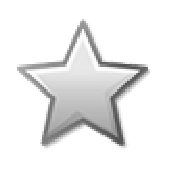
\includegraphics[width=0.7cm]{im/imagen_consejo} & \parbox{14cm}{\textbf{\underline{Consejo:}} #1}\\
	\end{tabular}
	\end{flushleft}
}

%% Ejemplo
\newcommand{\ejemplo}[1]{
	
	\begin{flushleft}
	\begin{tabular}{|cl|}
	\hline
	
	& 
\includegraphics[width=0.7cm]{im/imagen_ejemplo.eps}  \begin{large}Ejemplo\end{large}\\
	&\\
	&
	\begin{minipage}{17cm}
		\listinginput{1}{#1}
	\end{minipage} \\
	&\\
	\hline
	\end{tabular}
	\end{flushleft}
	
}




\begin{document}





\begin{center}
        \begin{Huge}
                \textsc{introducci�n al lenguaje C}
        \end{Huge}
        \vspace{7cm}
        

        \begin{tabular}{lr}
                \begin{minipage}{8cm}
                        \begin{center}
                                
\includegraphics{im/acm-big-logo.eps}
                        \end{center}
                \end{minipage}&
                \begin{minipage}{8cm}
                        \begin{large}
                                \textbf{ACM Cap�tulo de Estudiantes}
                                \vspace{0.5cm}\\
                                Facultad de Inform�tica, UPM
                                \vspace{0.5cm}\\
                                Marzo 2007

                        \end{large}
                        
                \end{minipage}\\
        \end{tabular}
\end{center}

\pagenumbering{gobble}
\newpage

\vspace*{18cm}
\section*{Introducci�n al lenguaje C}

{
\flushleft
\copyright 2003-2007 ACM Cap�tulo de Estudiantes - Facultad de Inform�tica UPM\\
ACM Cap�tulo de Estudiantes \\
Facultad de Inform�tica - Universidad Polit�cnica de Madrid \\
Campus de Montegancedo s/n \\
28660 Boadilla del Monte \\
MADRID (SPAIN)\\
}
Esta obra puede ser distribuida �nicamente bajo los t�rminos y condiciones
expuestos en \textbf{Creative Commons\\ \mbox{Reconocimiento-CompartirIgual}} 2.0 o
superior (puede consultarla en
\textit{http://creativecommons.org/licenses/by-sa/2.0/es/}).

\newpage

\pagenumbering{roman}

\tableofcontents
\listoffigures
\listoftables
\newpage

\pagestyle{headings}
\pagenumbering{arabic}

%\setcounter{chapter}{-1}

%
% PREFACIO
%
%%
% CAP�TULO: PREFACIO
%


\chapter*{Prefacio}

Desde hace varios a�os el Cap�tulo de Estudiantes ACM tiene 
como meta la difusi�n, uso y aprovechamiento en el entorno universitario de
las tecnolog�as disponibles por parte de los alumnos de esta
facultad. Por ello cada a�o organizamos talleres, concursos,
seminarios y cursos como el que tienes ahora en tus manos. Todos estos
eventos se realizan de manera gratuita o a un precio simb�lico, pol�tica que cada
a�o reafirma su �xito y aceptaci�n.\\


En ACM estamos convencidos del
beneficio que la actividad de la asociaci�n aporta a los
alumnos. Pero ello no ser�a posible sin la aportaci�n desinteresada
del tiempo y el esfuerzo de muchos compa�eros tuyos, alumnos como
t�, de los cuales una gran mayor�a un d�a asisti� a un evento ACM y
desde entonces decidi� participar de la actividad de la
asociaci�n.\\

Todos nosotros hemos aprendido de nuestros compa�eros de
asociaci�n, y esperamos que parte de ese conocimiento reporte ahora en
los asistentes a este evento.
Por lo tanto, s�lo nos queda invitarte a que participes en esta cadena
de compartici�n del conocimiento. Puedes encontrarnos 
en la p�gina \url{http://acm.asoc.fi.upm.es}\\



%%
%% INTRODUCCI�N
%%
%
% CAP�TULO: INTRODUCCI�N
%
\newpage
\ \
\newpage
\chapter{Introducci�n}
\section{Un poco de historia...}

El lenguaje de programaci�n C fue ideado e implementado por Dennis
Ritchie en 1972 en un DEC PDP-11\footnote{Un ordenador ``prehist�rico", enorme, con cintas, 
similar a los que salen en las pel�culas} usando UNIX como sistema operativo. Inicialmente, 
el est�ndar de C fue realmente la versi�n proporcionada por la 
implementaci�n de la versi�n V del sistema operativo UNIX. Su r�pida
expansi�n lleva a la aparici�n de varias variantes y problemas de
compatibilidad, por lo que en verano del 1983 se estableci� un comit�
para crear el est�ndar \textsc{ANSI}\footnote{Instituto Nacional de Est�ndares
Americano (American National Standards Institute)} para C. En 1989 se adopt� finalmente el est�ndar y poco despu�s
aparecieron los primeros compiladores conformes a este est�ndar. En 1995 se adopt� la 1� enmienda
con algunos cambios de la biblioteca de funciones, y fue la base para
desarrollar C++. Finalmente, en 1999 se adopt� el est�ndar C99 con
algunas mejoras e ideas prestadas de C++. Actualmente cohexisten las
dos versiones, mientras los programas migran a C99.

\section{Caracter�sticas}

\begin{itemize}
\item C es un lenguaje estructurado de nivel medio, ni de bajo
  nivel como ensamblador, ni de alto nivel como Ada o 
  Haskell. Esto permite una mayor flexibilidad y potencia, a cambio de
  menor abstracci�n.

\item No se trata de un lenguaje fuertemente tipado, lo que significa
  que se permite casi cualquier conversi�n de tipos. No es necesario que
  los tipos sean exactamente iguales para poder hacer conversiones,
  basta con que sean parecidos.

\item No lleva a cabo comprobaci�n de errores en tiempo de ejecuci�n,
  por ejemplo no se comprueba que no se sobrepasen los l�mites de los
  \textit{arrays}\footnote{Agrupaci�n de elementos de un mismo tipo de forma consecutiva  en memoria .
  Volveremos
  sobre los \textit{arrays} m�s tarde}. El programador es el �nico responsable de llevar a cabo esas
  comprobaciones.

\item Tiene un reducido numero de palabras clave, unas 32 en C89 y 37
  en C99. 
 
\item C dispone de una \emph{biblioteca est�ndar}
  que contiene numerosas funciones y que siempre est� disponible, adem�s de las extensiones que proporcione cada compilador o entorno
  de desarrollo.
\end{itemize} 

En resumen, es un lenguaje muy flexible, muy potente, muy popular,
pero que no protege al programador de sus errores.

\section{C frente a C++}

%Al principio es habitual no entender bien la diferencia entre C y C++,
%este �ltimo es un lenguaje para la programaci�n orientada a objetos
%que toma como base el lenguaje C. Se puede ver al C++ como una
%extensi�n de C para programaci�n orientada a objetos. \\

%En general, se puede utilizar un compilador de C++ para compilar un
%programa escrito en C, de hecho la mayor�a de los compiladores son
%para C/C++ indistintamente.

%----------------------------

No podemos hablar de C sin mencionar a C++, dado que es habitual no tener muy claro cuales 
son sus diferencias. En pocas palabras, C++ es un lenguaje para programaci�n orientada a objetos 
que toma como base el lenguaje C. La programaci�n orientada a objetos es otra filosof�a 
de programaci�n distinta a la de C (programaci�n estructurada)\footnote{ La programaci�n orientada a
objetos queda fuera del �mbito de este texto, para mas informaci�n se puede consultar cualquier libro de C++ } 
aunque con C++ es posible (aunque no especialmente recomendable) mezclar ambos estilos de programaci�n. 
En t�rminos generales, podemos ver a C++ como una extensi�n de C. Sin embargo, como se defini� 
a partir del est�ndar de C de 1989, y han evolucionado por separado, 
hay peque�as divergencias entre ellos.\\

Por lo general, se puede utilizar un compilador de C++ para compilar un 
programa escrito en C, inversamente la gran mayor�a de los programas 
escritos en C son v�lidos en C++. De hecho actualmente la mayor�a de los 
compiladores admiten tanto c�digo en C como en C++. 



\newpage

%%
%% HERRAMIENTAS
%%
\chapter{Herramientas y software para la programaci�n en C (entorno GNU/Linux)}

Aunque existen m�ltiples plataformas, mencionamos ahora s�lo las m�s
comunes: Microsoft Windows y GNU/Linux. En Windows disponemos de
herramientas propietarias de desarrollo en C (Microsoft Visual Studio,
Borland, etc) y herramientas de libre distrubuci�n (djgpp, gcc,
etc). Los productos propietarios suelen integrar varias
herramientas en un solo producto IDE\footnote{``suites'' que incorpor�n el
editor, manuales de referencia, compilador....} como Visual Studio, aunque
tambi�n podemos encontrar alg�n IDE de libre distribuci�n. En
cualquier caso, todas las herramientas de libre distrubuci�n que
podamos encontrar para GNU/Linux est�n disponibles para Windows (gcc,
gdb, wincvs, etc).\\

Tambi�n existen IDE's disponibles para GNU/Linux pero en
estas secciones no hablaremos de ellos. Recomendamos en cambio el uso
de las herramientas m�s extendidas y comunes en entornos UNIX. Y de
ellas son de las que hablaremos en las siguientes secciones.
Como es l�gico, la herramienta principal a la hora de programar en
cualquier lenguaje es el compilador (o el int�rprete en su caso). Pero
no es ni mucho menos la �nica herramienta de la que
disponemos. Tambi�n necesitaremos un editor de texto con el que
editaremos el c�digo fuente y, como veremos en este cap�tulo, tambi�n
disponemos de depuradores, sistemas de control de versiones, etc, que
facilitan enormemente la vida del programador.

\section{Compilador: \texttt{gcc}}
GCC\footnote{Originalmente acr�nimo de \textit{GNU C Compiler}. Actualmente se
refiere a \textit{GNU Compiler Collection}, debido a la posibilidad de compilar
otros lenguajes como Ada, Java o Fortran} es un compilador r�pido, muy flexible, y
riguroso con el est�ndar de C ANSI. Como ejemplo de sus m�ltiples
virtudes, diremos que gcc puede funcionar como \textit{compilador
cruzado}\footnote{un compilador cruzado corre bajo una arquitectura,
por ejemplo Intel x86, pero el c�digo binario que genera est� dise�ado
para correr en otra arquitectura distinta, por ejemplo SPARC} para un
gran n�mero de arquitecturas distintas. gcc no proporciona un entorno
IDEs, es solo una
herramienta m�s a utilizar en el proceso. gcc se encarga de realizar (o encargar el 
trabajo a otras utilidades, como veremos) el preprocesado 
(ver \ref{preprocesador}) del c�digo, la compilaci�n,
y el enlazado. Dicho de otra manera, nosotros proporcionamos a gcc
nuestro c�digo fuente en C, y �l nos devuelve un archivo binario
compilado para nuestra arquitectura.\\

Como curiosidad, mencionar que en realidad gcc no genera c�digo
binario alguno, sino c�digo ensamblado. La fase de
ensamblado a c�digo binario la realiza el ensamblador de GNU
(\textit{gas}), y el enlazado de los objetos resultantes, el enlazador
de GNU (\textit{ld}). Este proceso es transparente para el usuario, ya
que a no ser que se lo especifiquemos, gcc realiza el paso desde
c�digo en C a un binario ejecutable autom�ticamente.

\subsection{Manejo de gcc}

Casi siempre, gcc es invocado desde la herramienta \textit{make}, cuyo
funcionamiento se explica m�s adelante. Pero obviamente, debemos saber manejar
m�nimamente gcc para compilar nuestros programas. La sintaxis de gcc es la siguiente:

\begin{verbatim}
Usage: gcc [options] file...
\end{verbatim}

Vamos pues a compilar nuestro primer programa con gcc, que no podr�a
ser de otra manera, ser� un \textit{hola mundo}\footnote{el primer
ejemplo de cualquier tutorial de un lenguaje}:

\ejemplo{herramientas/holamundo.c}

y lo compilamos ejecutando:

\begin{verbatim}
mustang@amarok:~/seminarioc/documentacion/herramientas > gcc holamundo.c 
mustang@amarok:~/seminarioc/documentacion/herramientas > ls
total 68
drwxr-xr-x    4 mustang  mustang      4096 2003-10-30 14:07 .
drwxr-xr-x   16 mustang  mustang      4096 2003-10-30 13:43 ..
-rwxr-xr-x    1 mustang  mustang      5159 2003-10-30 14:00 a.out
-rw-r--r--    1 mustang  mustang        77 2003-10-30 14:00 holamundo.c
mustang@amarok:~/seminarioc/documentacion/herramientas > 
\end{verbatim}

Nos muestra un archivo \verb+a.out+, que es el archivo ejecutable
resultado de la compilaci�n. Lo ejecutamos:

\begin{verbatim}
mustang@amarok:~/seminarioc/documentacion/herramientas > ./a.out 
Hola mundo
mustang@amarok:~/seminarioc/documentacion/herramientas >
\end{verbatim}

Veamos como se comporta si introducimos un error en el fichero:

\ejemplo{herramientas/holamundo_error.c}

\begin{verbatim}
mustang@amarok:~/seminarioc/documentacion/herramientas > gcc holamundo_error.c
holamundo_error.c: In function `main':
holamundo_error.c:7: `a' undeclared (first use in this function)
holamundo_error.c:7: (Each undeclared identifier is reported only once
holamundo_error.c:7: for each function it appears in.)
holamundo_error.c:7: parse error before `return'
mustang@amarok:~/seminarioc/documentacion/herramientas >
\end{verbatim}

Como vemos gcc  nos proporciona el fichero y la l�nea en la que ha
detectado el error. El formato de la salida de error es reconocido por
la mayor�a de los editores, que nos permiten visitar esa posici�n con
atajos de teclado\footnote{en el editor Emacs, se puede hacer
  compilando mediante M-x compile, y usando el atajo C-x \`\
  SPC}. Obviamente, cuando gcc genera alg�n error, no se crea archivo
ejecutable como resultado.

\subsection{Warnings y errores}

\definicion{Error}{fallo al analizar el c�digo C que impide la
generaci�n de un ejecutable final.}

\definicion{\textit{Warning}}{advertencia del compilador al analizar
  el c�digo C que no impide la generaci�n de un ejecutable
  final.} 

Vamos a provocar que gcc se queje con un \textit{warning}. Para ello,
utilizamos el siguiente c�digo:

\ejemplo{herramientas/holamundo_warning.c}

Y lo compilamos con:

\begin{verbatim}
mustang@amarok:~/documentacion/herramientas > gcc -Wall holamundo_warning.c
holamundo_warning.c: In function `main':
holamundo_warning.c:6: warning: control reaches end of non-void function
mustang@amarok:~/documentacion/herramientas >
\end{verbatim}

\begin{flushleft}
A pesar del \textit{warning}, gcc ha compilado un fichero ejecutable. M�s
adelante veremos el significado de la opci�n \verb+-Wall+.
\end{flushleft}



\subsection{Opciones m�s comunes}

\label{opciones_gcc}

A continuaci�n mostramos algunas de las opciones m�s habituales al
usar gcc:

\begin{itemize}

\item{\texttt{--help}}

Indica a gcc que muestre su salida de ayuda (muy reducida).

\item{\texttt{-o <file>}}

El archivo ejecutable generado por gcc es por defecto \verb+a.out+. Mediante
este modificador, le especificamos el nombre del ejecutable. 

\item{\texttt{-Wall}}

No omite la detecci�n de ning�n warning. Por defecto, gcc omite una
colecci�n de warnings ``poco importantes''.

\item{\texttt{-g}}

Incluye en el binario informaci�n necesaria para utilizar un depurador
posteriormente. 

\item{\texttt{-O <nivel>}}

Indica a gcc que utilice optimizaciones en el c�digo. Los niveles
posibles van desde 0 (no optimizar) hasta 3 (optimizaci�n
m�xima). Utilizar el optimizador aumenta el tiempo de compilaci�n,
pero suele generar ejecutables m�s r�pidos.

\consejo{No utilices optimizaci�n cuando generes un ejecutable con informaci�n
de depuraci�n (opcion \texttt{-g}). Las optimizaciones introducidas pueden
confundir al depurador.}

\item{\texttt{-E}}

S�lo realiza la fase del preprocesador, no compila, ni ensambla, ni
enlaza.

\item{\texttt{-S}}

Preprocesa y compila, pero no ensambla ni enlaza.

\item{\texttt{-c}}

Preprocesa, compila y ensambla, pero no enlaza.

\item{\texttt{-I <dir>}}

Especifica un directorio adicional donde gcc debe buscar los archivos
de cabecera indicados en el c�digo fuente (ver \ref{include}).

\item{\texttt{-L <dir>}}

Especifica un directorio adicional donde gcc debe buscar las librer�as
necesarias en el proceso de enlazado (ver \ref{enlazado}).

\item{\texttt{-l<library>}}

Especifica el nombre de una librer�a adicional que deber� ser
utilizada en el proceso de enlazado (ver \ref{enlazado}).

\end{itemize}

La colecci�n completa de modificadores a utilizar con gcc se encuentra
en su p�gina de manual, \verb+man gcc+, cuyo manejo se explica un poco
m�s adelante (ver \ref{man}).


\section{Depuradores: \texttt{gdb} y \texttt{ddd}}
\label{gdb}

\definicion{Depurador}{Herramienta que permite al programador seguir la
ejecuci�n de su programa paso a paso, as� como ver el contenido de variables.}

\subsection{Depurando con \texttt{gdb}}

Para poder ejecutar un depurador sobre nuestros programas en C,
debemos especificar a gcc que incluya informaci�n de depuraci�n en los
binarios que genere. Como se vio en \ref{opciones_gcc}, en el caso de utilizar
gcc compilamos el programa 
con el modificador \texttt{-g}. 

\subsection{Depurador gr�fico: \texttt{ddd}}

DDD es un interfaz gr�fico para el depurador gdb. La principal ventaja
de ddd es la facilidad para mostrar los contenidos de las posiciones
de memoria durante la ejecuci�n de nuestro programa, como puede verse
en la siguiente captura:

\begin{figure}[H]
\begin{centering}
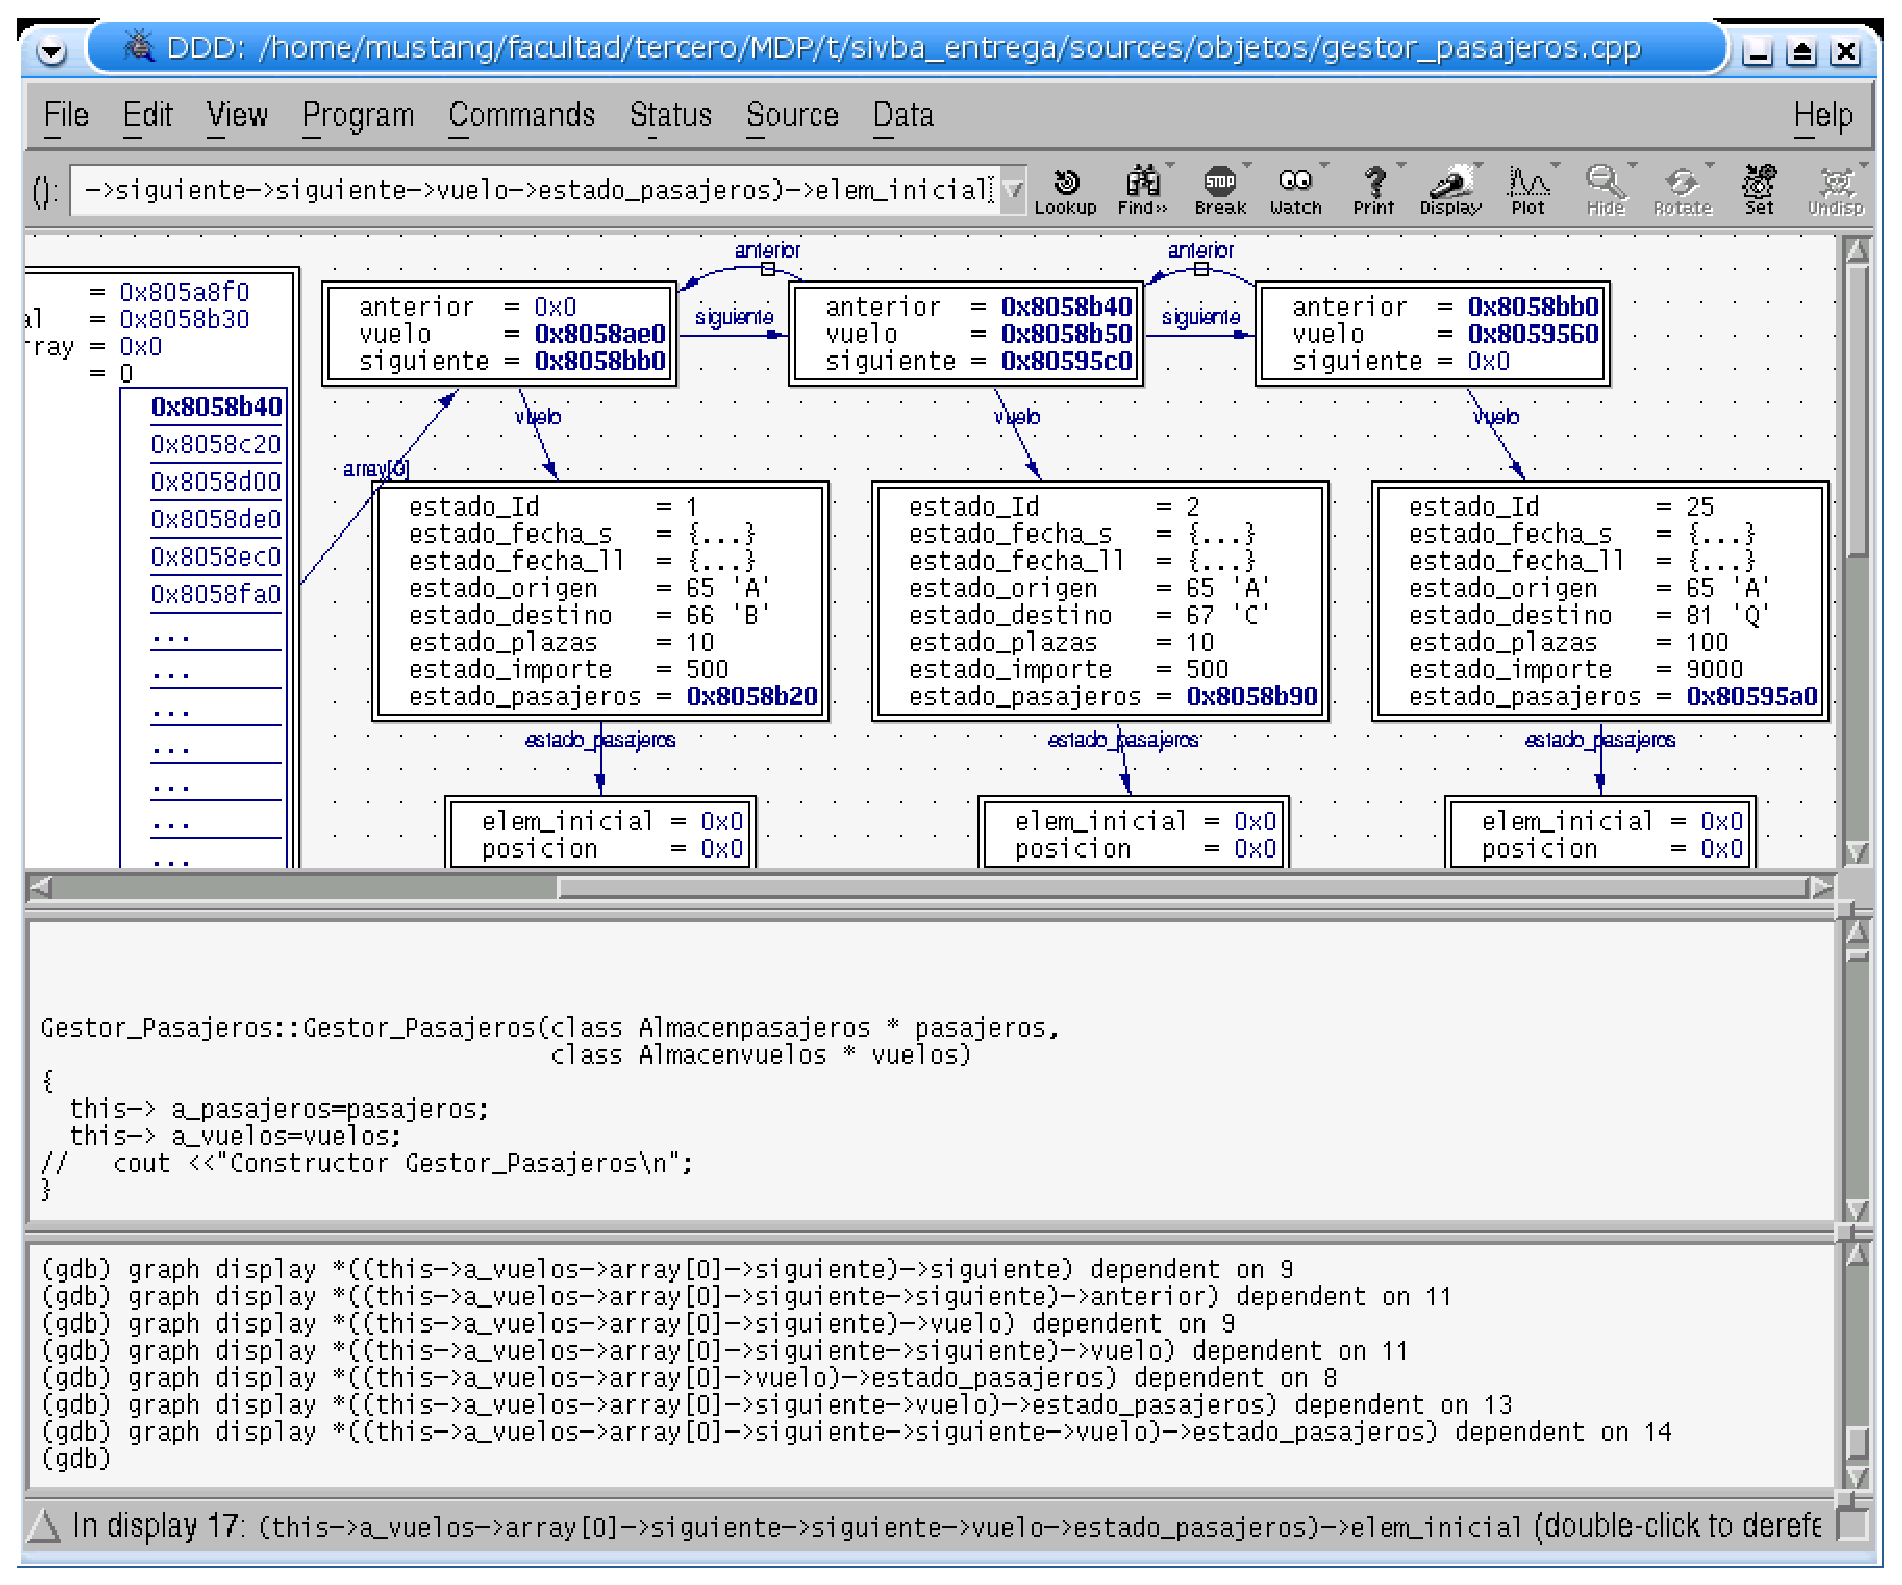
\includegraphics[width=18cm]{herramientas/ddd.eps}
\caption{DDD en accion, cadenas enlazadas}
\end{centering}
\end{figure}

\subsection{Manejo}

Para obtener una descripci�n del manejo de gdb y ddd, os remitimos a
la documentaci�n de un seminario previo de ACM: \cite{Adan}.


\section{Control de dependencias: \texttt{make}}
La mayor�a de nuestros proyectos de programaci�n
no constar�n de un solo fichero fuente sino de varios (puede
incluso que de centenas de ellos). Cuando editamos un fichero de c�digo
fuente y lo modificamos pasamos a compilarlo (con GCC o cualquier otro
compilador). Hay tener en cuenta que puede haber otros ficheros de
c�digo fuente que dependan del que acabamos de modificar. Por lo tanto, esos
ficheros de c�digo fuente que dependen del que acabamos de modificar
tambi�n deben ser compilados. La herramienta make nos evita la tediosa
tarea de compilar las dependencias, por no hablar de que nos
evita la necesidad de tener presente en todo momento cuales son las
dependencias entre ficheros de c�digo fuente. Para ello nos valemos de
un fichero (t�picamente con nombre \texttt{Makefile}) en el que
declaramos las dependencias entre ficheros de c�digo fuente y las
�rdenes necesarias para actualizar cada fichero. Una vez escrito el
fichero \texttt{Makefile}, cada vez que cambiemos alg�n fichero
fuente, con la orden:
\begin{verbatim}
make
\end{verbatim}
basta para que se realicen todas las recompilaciones necesarias.
Veamos ahora el formato b�sico del fichero \texttt{Makefile}.
El fichero Makefile m�s simple est� compuesto por ``reglas'' de este
aspecto.
\begin{verbatim}
objetivo ... : prerrequisitos ...
            comando
            ...
            ...
\end{verbatim}

Un objetivo suele ser el nombre de un fichero generado por un
programa; ejemplos de objetivos son ficheros ejecutables u objetos. Un
objetivo puede ser tambi�n el nombre de una acci�n a llevar a cabo,
como ``clean'', que veremos m�s adelante en un ejemplo.\\

Un prerrequisito es un fichero que se usa como entrada para crear un
objetivo. Un objetivo con frecuencia depende de varios ficheros.\\

Un comando es una acci�n que \texttt{make} ejecuta. Una regla puede
tener m�s de un comando, cada uno en su propia
l�nea. \emph{\bf{Atenci�n}:} �hay que poner un tabulador al
principio de cada l�nea de comando!\\

Normalmente un comando est� en una regla con prerrequisitos y
contribuye a crear un fichero objetivo si alguno de los prerrequisitos
cambia. Un ejemplo de excepci�n a esto es el objetivo ``clean'', que no
tiene prerrequisitos. Una regla, por tanto, explica como y cuando
reconstruir ciertos ficheros que son objetivos de reglas.\\

A continuaci�n tenemos un ejemplo de un Makefile que describe la manera en la
que un fichero ejecutable llamado ``edit'' depende de ocho
ficheros objeto que a su vez dependen de ocho ficheros de c�digo
fuente C y tres archivos de cabecera. Los ocho ficheros de c�digo
fuente C dependen del archivo de cabecera ``defs.h'' (como dijimos
anteriormente, mediante la directiva \texttt{\#include}). S�lo los
ficheros de c�digo que definen los comandos de edici�n dependen de
``command.h'', y s�lo los ficheros de operaciones de bajo nivel que
cambian el buffer del editor dependen de ``buffer.h''.

\begin{verbatim}
edit: main.o kbd.o command.o display.o \
      insert.o search.o files.o utils.o
       gcc -o edit main.o kbd.o command.o display.o \
             insert.o search.o files.o utils.o

main.o : main.c defs.h
       gcc -c main.c

kbd.o : kbd.c defs.h command.h
       gcc -c kbd.c

command.o : command.c defs.h command.h
       gcc -c command.c

display.c : display.c defs.h buffer.h
       gcc -c display.c

insert.o : insert.c defs.h buffer.h
       gcc -c insert.c

search.o : search.c defs.h buffer.h
       gcc -c search.c

files.o : files.c defs.h buffer.h command.h
       gcc -c files.c

utils.o : utils.c defs.h
       gcc -c utils.c

clean :
       rm -f edit *.o

\end{verbatim}

En el ejemplo dividimos cada l�nea larga en dos l�neas usando la
contrabarra\footnote{El car�cter $\backslash$}. Para crear el fichero ejecutable
  ``edit'', escribimos: 
\begin{verbatim}
make
\end{verbatim}
Para borrar el fichero ejecutable y todos los ficheros objeto del
directorio, escribimos:
\begin{verbatim}
make clean
\end{verbatim}

En el fichero Makefile del ejemplo, son objetivos el fichero
ejecutable ``edit'' y los ficheros objeto ``main.o'' y ``kbd.o'', entre
otros. Son prerrequisitos ficheros como ``main.c'' y ``defs.h''. De hecho,
cada fichero ``.o'' es tanto objetivo como prerrequisito. Son comandos
``gcc -c main.c'' y ``gcc -c kbd.c''.\\

Cuando un objetivo es un fichero, necesita ser recompilado si
cualquiera de los prerrequisitos cambia. Adem�s, cualquier
prerrequisito que es generado autom�ticamente deber�a ser actualizado
primero. En el ejemplo, ``edit'' depende de cada uno de los ocho
ficheros objeto; el fichero objeto ``main.o'' depende a su vez del fichero de
c�digo fuente ``main.c'' y del fichero de cabecera ``defs.h''. \\

Un comando de shell sigue a cada l�nea que contiene un objetivo y
prerrequisitos. Estos comandos de shell indican como actualizar el
fichero objetivo. Recuerda que hay que poner un tabulador al principio
de cada l�nea de comando para distinguir l�neas de comando de otras
l�neas en el Makefile. (Ten en cuenta que \texttt{make} no sabe nada
sobre c�mo funcionan los comandos. Depende de t� proporcionar los
comandos que actualizaran los ficheros objetivos de manera apropiada).\\

El objetivo ``clean'' no es un fichero, es simplemente el nombre de una
acci�n. Tampoco es un prerrequisito de otra regla ni tiene
prerrequisitos. Por tanto, \texttt{make} nunca har� nada con este
objetivo a no se que se le pida espec�ficamente.\\

Con esto hemos visto el funcionamiento m�s esencial de la herramienta
\texttt{make}. Pero \texttt{make} es mucho m�s. En la bibliograf�a
podemos encontrar referencias a documentaci�n m�s extensa de
\texttt{make}. 


\section{Manuales: \texttt{man}}
\label{man}

\verb+man+\footnote{El nombre del comando viene de \texttt{manual}} es un mandato de Unix/Linux que nos informa sobre el funcionamiento de
otros mandatos.
El funcionamiento de man no s�lo se limita a informarnos sobre el uso
de mandatos, nos informa tambi�n de funciones de libreria y llamadas a
funciones del sistema. Los archivos de manual de \verb+man+ se encuentran organizados en 9 secciones, de
las cuales, ahora s�lo estamos interesados en las 3 primeras:\\

\begin{tabular}{c|l}
\textbf{Secci�n} & \textbf{Descripci�n} \\
\hline
      1 &  Programas ejecutables y comandos de la shell \\
          \hline
       2 &  Llamadas al sistema\\
           \hline
       3  & Llamadas a funciones de biblioteca \\
           \hline
\end{tabular}
\vspace{0.4cm}
%\begin{flushleft}
%Existen 6 secciones m�s pero no nos interesan para la programaci�n en C.
%\end{flushleft}

Antes de comenzar a utilizar  \verb+man+ es recomendable que nos informemos m�s
sobre su utilizaci�n (\verb+man man+).
Aqui encontraremos algunas opciones muy �tiles:\\

\begin{tabular}{c|l}
\textbf{Opci�n} & \textbf{Descripci�n} \\
\hline
     -a &  Muestra de forma consecutiva las secciones en que existe manual del comando \\
     \hline
     -k &  Muestra las paginas de manual y secciones en que se hace referencia a lo buscado \\
     \hline
\end{tabular}
\vspace{0.4cm}

En el momento de buscar informaci�n 
debemos tener en cuenta que algunas funciones y
mandatos se encuentran en varias secciones 
y, por lo tanto, deberemos indic�rselo al man antes de su ejecuci�n. Para
especificar la secci�n sobre la que queremos consultar, lo haremos de la
siguiente forma: 
\begin{verbatim}
        man [n� seccion] [mandato]
\end{verbatim}


Como ejemplo de la utilizaci�n de \verb+man+, consultemos el uso de printf como llamada a funci�n de biblioteca, mediante la siguiente linea:
\begin{verbatim}
        man 3 printf
\end{verbatim}

Ahora veamos su uso como comando de la Shell:
\begin{verbatim}
        man 1 printf
\end{verbatim}





\section{Control Concurrente de Versiones: \texttt{cvs}}

CVS significa \textit{Concurrent Version System}. Es una herramienta
que nos permite mantener nuestro trabajo en un \textbf{repositorio},
al que m�ltiples usuarios pueden conectarse y realizar cambios. En
nuestra opini�n, es una de las mejores ayudas para el trabajo en
equipo, e incluso, para el trabajo individual (control de cambios en
las versiones). 

\subsection{Escenario de uso}

El usuario crea un repositorio en una m�quina, que almacenar� el
proyecto en el que se va a trabajar. Cada vez que se crea un archivo
nuevo en el proyecto, o un subdirectorio, se introduce en el repositorio
con un n�mero de versi�n inicial. Una vez creado el repositorio, cada usuario puede conectarse con el
servidor y descargarse una copia del mismo a su m�quina, trabajar con
los ficheros, y enviar los cambios al servidor. \\

Donde se nota realmente la potencia del sistema es cuando los
usuarios trabajan sobre los mismos ficheros. Mientras los cambios sean
en zonas diferentes de un mismo fichero, CVS se encarga de mezclar las
versiones sin interacci�n del usuario. El �nico escenario que requiere
intervenci�n del usuario es el siguiente:

\begin{itemize}
\item el usuario A se descarga la versi�n 1.3 del fichero X
\item el usuario B se descarga la versi�n 1.3 del fichero X
\item el usuario A modifica el fichero X y lo sube, generando la
  versi�n 1.4
\item el usuario B modifica el fichero X en el mismo sitio y lo sube,
  produciendo un conflicto con los cambios del usuario A
\end{itemize}

En este caso, CVS avisa al usuario B de que tiene que reconciliar a
mano ambas versiones, y le proporciona las diferencias entre sus
modificaciones y las de su compa�ero. Una vez que el usuario B corrige
a mano esos cambios, sube el fichero, generando la version 1.5.\\

CVS proporciona otras muchas ventajas, como poder generar ramas a
partir de un punto del proyecto, permitiendo que los usuarios trabajen
en ramas distintas, y muy importante, permite recuperar cualquier
versi�n de cualquier archivo existente. Podemos, por ejemplo,
recuperar un archivo tal y como estaba hace un mes.\\

A continuaci�n se muestra un ejemplo de operaci�n sobre un
repositorio:

\begin{verbatim}
Borrado gdb.tex, ya no era necesario
Cambios en las tildes de cvs.
CVS: ----------------------------------------------------------------------
CVS: Enter Log.  Lines beginning with `CVS:' are removed automatically
CVS: 
CVS: Committing in .
CVS: 
CVS: Modified Files:
CVS:    cvs.tex 
CVS: Removed Files:
CVS:    gdb.tex 
CVS: ----------------------------------------------------------------------
\end{verbatim}


\subsection{Manejo}

Os remitimos a la estupenda documentaci�n realizada por un compa�ero
de ACM en \cite{Hernando}.


\section{Herramientas de desarrollo C sobre Windows}

Cuando utilizamos Windows no tenemos tan claro que compilador utilizar
ya que en Windows disponemos de herramientas portadas de Linux
(gcc.exe) o las herramientas que Microsoft nos proporciona para
desarrollar programas (Visual Studio) que podemos obtener de
Biblioteca con una licencia de estudiante de forma gratuita.

\subsection{GCC en Windows}

La compilaci�n de un programa utilizando el GCC se realiza de la misma
forma a la vista en Linux, pero debemos tener en cuenta que no todo
programa que compile en Linux compila en Windows debido a las
diferencias existentes en las llamadas al sistema. Esto es debido a  que Windows
no cumple completamente con el estandar POSIX (ver \ref{posix}) de llamadas al sistema. 
Estas
herramientas para Windows las podemos obtener por medio de diferentes
programas, ya sea bajandonos el conjunto de herramientas UNIX para
Windows \textit{MinGW}, o descarg�ndonos desde la facultad el compilador
de Ada95 \textit{(GNAT)}, el cual viene con un el GCC, ya que la
compilaci�n llevada a cabo por \textit{GNATMAKE} es una traducci�n del
lenguaje Ada a C y una posterior compilaci�n en C.  Estas herramientas
estan disponibles desde las siguientes direcciones:

\begin{itemize}
\item \url{ftp://lml.ls.fi.upm.es/pub/lenguajes/ada/gnat/3.13p/winnt/}
\item \url{http://www.mingw.org/download.shtml}
\end{itemize}

%Si nos decantamos por la utilizaci�n del GCC proporcionado por \textit{GNATMAKE} deberemos
%tener en cuenta que los programas que queramos compilar deben ser copiados a la ruta ...
Y recordad, tanto si elegimos utilizar el paquete de utilidades Linux
que encontramos en \textit{MinGW}, como si elegimos el \textit{GNAT},
deberemos incluir la ruta donde instalemos estos archivos en nuestro
\verb+PATH+ para que funcione la compilaci�n. Otra posibilidad es
crear todos los archivos dentro de la carpeta donde se encuentre
instalado \textit{MinGW} o el archivo \verb+gcc.exe+ ya que en caso
contrario, Windows no podra localizar el compilador \verb+gcc+ y nos
mostrara ese maravilloso mensaje de error:

\begin{verbatim}
"gcc" no se reconoce como un comando interno o externo, programa o
archivo por lotes ejecutable.
\end{verbatim}

% \subsection{Visual Studio}
% 
% Si decidimos utilizar como herramienta de compilaci�n este programa,
% nos encontraremos con un interfaz de desarrollo orientado a proyectos
% con C++ pero podremos utilizarlo tambien para compilar nuestros
% programas en C.
% 
% Tambi�n mencionaremos aqu� la depuraci�n disponible en Visual Studio,
% el cual nos permitira visualizar los valores de las direfentes
% variables, desde su valor en memoria y la ejecuci�n paso a paso de
% cada una de las lineas de c�digo.
% 
% \subsection{Depuracion: \texttt{gdb}}
% 
% En Windows, al igual que pasaba con el gcc, disponemos de un GDB
% portado desde Linux, el cual funciona de identica manera a la
% explicada en la secci�n \ref{gdb}.


\newpage

%%
%% SINTAXIS 
%%

\newpage
\ \
\newpage
%% SECCI�N: SINTAXIS DE PUNTEROS

\section{Sint�xis de punteros}

\subsection{Declaraci�n de punteros}

Ante todo, \emph{un puntero es una variable}. Al dedicar un inter�s
especial en los punteros, puede dar la impresi�n de que son elementos
separados de las variables. No es as�. Son variables, y como veremos,
podemos asignarles nuevos valores, e incluso realizar algunas
operaciones aritm�ticas �tiles con ellos.\\

\emph{Una variable de tipo puntero est� �ntimamente ligada con el tipo
  al que apunta}. Por ello, en la declaraci�n, escribimos el nombre
  del tipo al que apuntar� nuestro puntero, seguido de asterisco, y por
  �ltimo, el nombre del puntero. Ejemplo:

\begin{verbatim}
int *p_entero;
float *p_real;
char *caracter;
\end{verbatim}

Ser�n declaraciones de punteros que contendr�n la direcci�n de memoria
de un entero, un real y un car�cter\footnote{Como veremos, la
  declaraci�n char * es usada tambi�n para la declaraci�n de
  cadenas de caracteres} respectivamente.

\subsection{Punteros gen�ricos}

Un caso especial, es cuando queremos declarar un puntero ``gen�rico'',
esto es, queremos que el puntero no est� ligado a ningun tipo
concreto. �Qu� sentido tiene esto?, como se ha visto previamente, en C
podemos realizar un \textit{cast} (ver \ref{cast}) sobre una variable,
y forzar su conversi�n a otro tipo. De esta manera, por ejemplo,
podr�amos declarar un puntero gen�rico, apuntar a una zona de memoria,
y realizar un cast sobre el puntero gen�rico.
\nota{La �nica diferencia existente entre un puntero
gen�rico, y un puntero ligado a un tipo de datos concreto, se produce
en las operaciones de aritm�tica de punteros (ver
\ref{punteros_aritmetica}).} 

Para declarar un puntero de tipo gen�rico, utilizamos:

\begin{verbatim}
void * pointer;
\end{verbatim}

Como veremos, muchas funciones de biblioteca de POSIX manejan punteros
gen�ricos en sus argumentos.

\subsection{Los operadores de contenido ``\texttt{*}'' y de indirecci�n
  ``\texttt{\&}''} 

\label{operadores_punteros}

El operador de indirecci�n \texttt{\&} se utiliza para referirse a la
direcci�n de una variable, as� el c�digo siguiente:

\begin{verbatim}
/* Reservamos 4 bytes para almacenar una direcci�n de memoria */
int *p_entero;

/* Reservamos 4 bytes para almacenar un entero */
int entero;

/* Escribimos en la variable p_entero la direcci�n de entero */
p_entero = &entero;
\end{verbatim}

Es totalmente correcto ya que, aunque la variable \texttt{entero} no
tenga ning�n valor asignado todav�a, lo que estamos haciendo es
escribir en la variable \texttt{p\_entero} la direcci�n de memoria
donde se almacena la variable \texttt{entero}.\\

\begin{figure}[H]
\begin{centering}
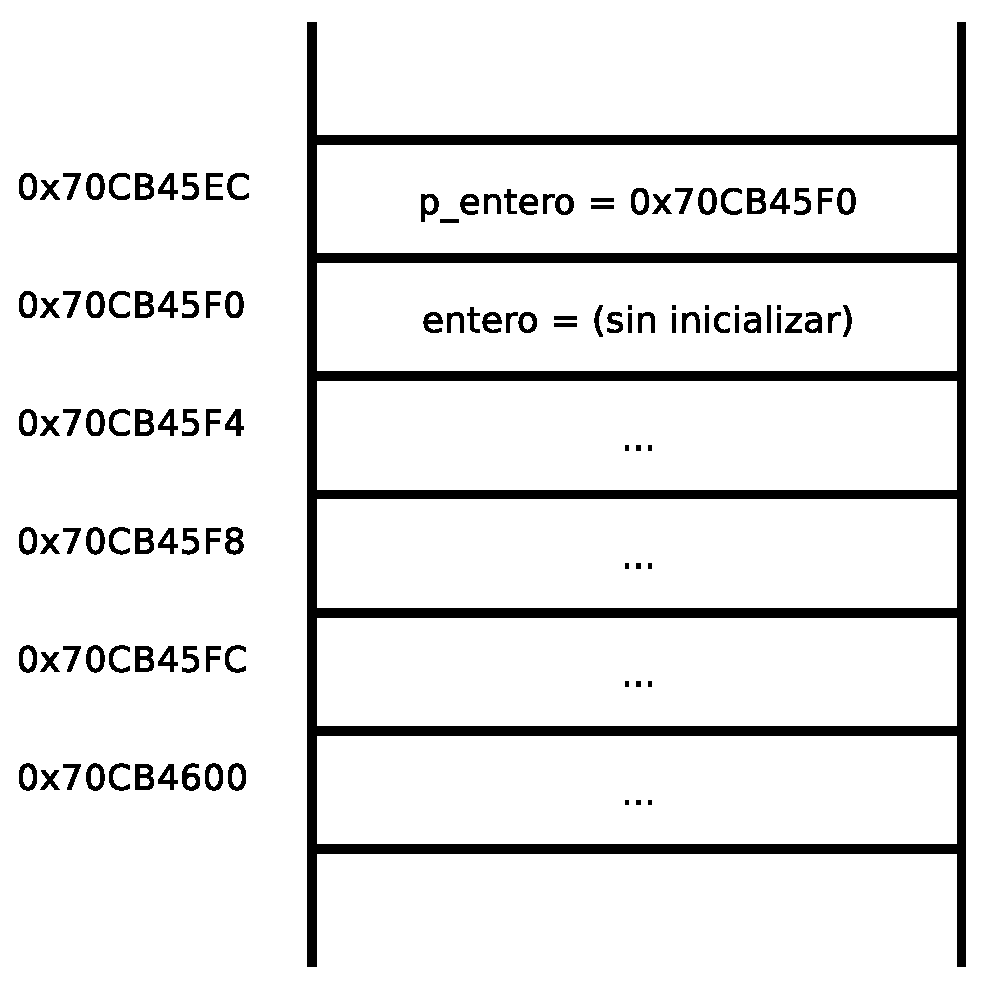
\includegraphics[width=80mm]{punteros/images/init_punteros.eps}
\caption{Inicializando punteros}
\end{centering}
\end{figure}

El operador \texttt{*} se utilizar para manejar la direcci�n a la que
apunta un puntero. Podr�amos llamarlo el operador de
\textit{acceso}. Tanto el operador de acceso, como el de indirecci�n,
funcionan en \textbf{notaci�n prefija}. Veamos un ejemplo que combina
ambos operadores:

\begin{verbatim}
1 int *p_entero;
2 int entero1, entero2;
3 entero1 = 2;
4 entero2 = 5;
5 p_entero = &entero1;
6 entero1 = *p_entero + entero2;
\end{verbatim}

Del mismo modo podemos asignar un valor a la variable a la que apunta
el puntero, de la forma:

\begin{verbatim}
1 int *p_entero;
2 int entero1, entero2;
3 entero1 = 2;
4 entero2 = 5;
5 p_entero = &entero1;
6 *p_entero = entero1 + entero2;
\end{verbatim}

Este �ltimo c�digo ejecutar�a \textbf{exactamente} lo mismo que el
anterior. Debemos notar que no tendr�a sentido prescindir de la linea
5, puesto que estar�amos intentando introducir el valor
\texttt{entero1 + entero2} en una direcci�n de memoria que no
conocemos, puesto que no le habriamos dado valor a \texttt{p\_entero}
(ver \ref{punteros_roma}).

\newpage


%%
%% MODELO DE COMPILACION
%%

\newpage
\ \
\newpage

%
% CAP�TULO: EL MODELO DE COMPILACI�N DE C
%
\chapter{El modelo de compilaci�n de C}
\label{chapter:comp}

%
% SECCI�N: INTRODUCCI�N
%
\section{Introducci�n}


En este cap�tulo vamos a ver c�mo es el modelo de compilaci�n en C, es decir, por qu� 
fases pasa nuestro c�digo desde que lo editamos hasta que obtenemos un fichero ejecutable.
En principio uno podr�a pensar que conocer lo que ocurre ``por debajo'' no es necesario
a  la hora de programar C, y de hecho no estar�a muy equivocado. Sin embargo hay ciertos
procesos que ocurren cuando compilamos nuestro c�digo C que como programadores debemos
conocer.

\begin{flushleft}
El proceso de compilaci�n de c�digo C consta de tres fases principales:
\end{flushleft}

\begin{enumerate}
	\item{\textbf{Preprocesado}}
	\item{\textbf{Compilado}}
	\item{\textbf{Enlazado}}
\end{enumerate}

Primera sorpresa: La compilaci�n es solo una fase del proceso de compilaci�n. Esta aparente
contradicci�n se explica f�cilmente: cuando hablamos del proceso de compilaci�n nos estamos
refiriendo al proceso mediante el cual transformamos nuestro c�digo fuente en un fichero
ejecutable. Sin embargo cuando nos referimos a la fase de compilaci�n nos estamos refiriendo
a la parte del proceso que se encarga de traducir c�digo fuente en instrucciones en formato
binario.



% seccion El preprocesador
\section{El preprocesador}
\label{preprocesador}

El preprocesador es algo caracter�stico de C/C++, que no se suele encontrar en otros lenguajes
 de programaci�n. El preprocesador act�a sobre el programa fuente, antes de que empiece 
la compilaci�n propiamente dicha, para realizar ciertas operaciones.\\


Una de estas operaciones es, por ejemplo, la sustituci�n de constantes simb�licas, 
como vimos en el cap�tulo de constantes. Tambi�n permite definir macros, 
que son parecidas a funciones, \emph{pero no iguales}, y realizar compilaci�n condicional. 
En general se encarga de modificar el c�digo fuente, seg�n una serie de directivas. 
Estas se reconocen puesto que empiezan por \verb-#- y no tienen 
que terminar en \verb-;-, a diferencia de las instrucciones de C.


\subsection{\texttt{\#include}: inclusi�n de otros ficheros}
\label{include}
Cuando en un archivo de c�digo fuente se encuentra una l�nea con un \verb-#include- 
seguido de un nombre de archivo, el preprocesador \emph{incluye} el archivo 
en el punto donde se encuentra la directiva, exactamente igual que si hici�ramos copiar/pegar. 
La sintaxis de este comando es la siguiente: 
\begin{verbatim}
#include "nombre_del_archivo" 
\end{verbatim}
o
\begin{verbatim}
#include <nombre_del_archivo> 
\end{verbatim}
La diferencia entre la primera forma (con comillas \verb-"-\ldots\verb-"-) y la segunda forma 
(con los s�mbolos \verb-<-\ldots\verb->-) est� en el directorio de b�squeda de los archivos 
a incluir. En la forma con comillas se busca el archivo en el directorio actual y posteriormente 
en el (o los) directorio(s) est�ndar de librer�as\footnote{los directorios de librer�as dependen del sistema operativo y compilador que se use}. 
En la forma que utiliza los s�mbolos \verb-<-\ldots\verb->- se busca directamente en el 
directorio est�ndar de librer�as, sin buscar en el directorio actual. 

\consejo{Los archivos de la librer�a est�ndar (stdio.h, math.h, etc...) 
se suelen incluir con \texttt{<...>} mientras que los archivos hechos por el propio programador 
se ponen entre comillas. Es una cuesti�n de costumbre m�s que otra cosa.}

Los archivos incluidos pueden contener a su vez directivas \verb-#include-, esto se conoce como 
inclusi�n anidada. El n�mero de niveles de anidamiento depende del compilador, pero ha de ser 
al menos 8 en C89 y 15 en C99 (en cualquier caso es m�s que de sobra).\\

Este comando del preprocesador se utiliza normalmente para incluir las cabeceras 
(\textit{headers} en ingl�s). Estos son archivos con los prototipos de las funciones de librer�a o 
con las funciones definidas para el programa en cuesti�n\footnote{las cabeceras son 
el equivalente en C/C++ de los archivos ``.ads" de ADA}.

\subsection{\texttt{\#define:} creaci�n de macros}

Como vimos, con la directiva \verb-#define- se define un \textit{alias}, es decir una sustituci�n de texto. 
Esto, que us�bamos para definir constantes, se puede utilizar de la misma manera para definir macros. 
En efecto, podemos poner par�metros a esas sustituciones, que se comportan entonces como si de una
pseudo-funci�n se tratara.\\

En una macro con argumentos, los argumentos se sustituyen en el texto de reemplazo, 
y a continuaci�n la macro se \emph{expande}, es decir, en el programa el texto de reemplazo reemplaza al identificador y a la lista de argumentos.\\
Veamos por ejemplo:

\begin{verbatim}
#define PI 3.14
#define AREA_CIRCULO(x) PI * (x) * (x)
\end{verbatim}

\begin{flushleft}
Ahora podemos usar la macro como si fuera funci�n normal:
\end{flushleft}

\begin{verbatim}
void main() { 
   int a;
   a = AREA_CIRCULO(3); 
}
\end{verbatim}

\begin{flushleft}
Durante la compilaci�n la macro se expande a:
\end{flushleft}

\begin{verbatim}
  a = 3.14 * (3) * (3)
\end{verbatim}
y obtenemos el resultado esperado.\\

Las macros nos permiten insertar c�digo en el programa directamente, evitando la sobrecarga
de invocar a una funci�n (pasar par�metros a la pila, realizar un salto, 
recibir par�metros \ldots)\footnote{En C++ se puede hacer lo mismo usando la directiva \emph{inline}.} pero conservando la legibilidad del programa. 
Por otra parte permite realizar c�lculos durante la compilaci�n, en lugar de realizarlos 
durante la ejecuci�n. As� en el ejemplo que nos ocupa el compilador le da directamente el valor
adecuado a la variable ``a", en lugar de insertar instrucciones para que se eval�e cada vez que se use.\\

Es importante no olvidar los \textsc{par�ntesis} alrededor de los par�metros en la definici�n
de la macro, de lo contrario la expansi�n de par�metros puede ser incorrecta, por ejemplo:
\begin{verbatim}
#define AREA_CIRCULO(x) PI * x * x
void main() { 
   int a,b;
   a = AREA_CIRCULO(c + 3); 
}
\end{verbatim}
expande a:
\begin{verbatim}
  a = 3.14 * c + 3 * c + 3
\end{verbatim}
que, por culpa de la precedencia de operadores, es equivalente a 
\begin{verbatim}
  a = (3.14 * c) + (3 * c) + 3
\end{verbatim}
en lugar de expandir a:
\begin{verbatim}
  a = 3.14 * (c + 3) * (c + 3)
\end{verbatim}
que es lo que quer�amos.


\subsection{Compilaci�n condicional}

Hay varias directivas que permiten compilar selectivamente partes del c�digo fuente del programa. 
Este proceso se llama \emph{compilaci�n condicional} y se utiliza mucho cuando se quiere mantener
versiones diferentes de un programa. Por ejemplo se puede mantener una versi�n demo o recortada,
gratuita y otra mas potente de pago, y las partes de c�digo que difieran entre las dos se compilan 
seg�n sea la plataforma de destino.
\subsubsection{uso de \#if, \#else, \#elif y \#endif} 
Estas directivas permiten incluir parte del c�digo seg�n el valor que tome una constante de preprocesador.\\
Veamos un ejemplo:
\begin{verbatim}
#define MAX 10

int main(void){
#if MAX > 99
   printf("versi�n PRO, compilada para arrays mayores de 99.\n");
   ...
#else
   printf("versi�n DEMO, compilada para arrays menores de 99.\n");
   ...
#endif
   return 0;
}
\end{verbatim}
Aqu�, al ser MAX menor de 99 el bloque que sigue al \verb-#if- no se compila, en su lugar se 
compila la alternativa del bloque \verb-#else-.\\

Se pueden hacer selecciones m�ltiples mediante \verb-#elif- que equivale a ``else if"

\subsubsection{uso de \#ifdef , \#ifndef y \#undef}

Estas directivas permiten compilaci�n condicional bas�ndose en si esta definida una macro o no,
independientemente del valor que tenga. Se usan a menudo para tener una versi�n de prueba con
chequeos adicionales (de rangos, de correcci�n de par�metros\ldots ), y otra final, sin ellos 
(y por tanto m�s r�pida).\\

\nota{No es mala idea definir una macro DEBUG, por ejemplo, que permita alternar entre
compilaci�n con chequeos extra y versi�n final}

Con \verb-\#undef- podemos ``desdefinir'' una definici�n previamente realizada.



% seccion Compilaci�n enlazada
\section{Compilaci�n}

La compilaci�n es la fase m�s costosa del proceso de compilaci�n y esto es
debido a que el compilador debe analizar el texto de nuestro programa fuente,
comprobar que no contiene errores  y producir como salida un fichero con la traducci�n de nuestro
c�digo a conjunto de instrucciones de nuestro procesador.\\


Ning�n proyecto de programaci�n serio est� compuesto hoy en d�a por un solo archivo fuente, sino 
m�s bien todo lo contrario. Es conveniente que cualquier programa que pase de unos cientos de
l�neas sea dividido en una serie de m�dulos que faciliten la legibilidad y el mantenimiento del
c�digo.\\

A la hora de compilar nuestro proyecto lo que haremos ser� \textit{procesar} cada uno
de estos m�dulos por separado, dici�ndole al compilador que tenga en cuenta que ninguno
de estos m�dulos es un programa por si mismo, sino una parte del mismo. Lo que har� el compilador
ser� producir como salida una serie de \textbf{ficheros objeto}\footnote{La extensi�n habitual
de estos ficheros es \texttt{.o} (Unix/Linux) o \texttt{.obj} (Windows)}. Estos ficheros son la traducci�n
a binario de cada uno de nuestros m�dulos. Sin embargo ninguno de ellos conforma un ejecutable
por s� mismo, ya que ninguno contiene el c�digo completo de nuestro programa.

%
% SECCI�N: ENLAZADO
%
\section{Enlazado}

\label{enlazado}

La fase de enlazado consiste simplemente en ``reunir'' cada uno de los ficheros objeto
producidos en la fase anterior, resultando de este proceso un fichero ejecutable. Si nuestro
programa hace uso de librer�as externas (la mayor�a lo hacen), el c�digo de las funciones
utilizadas ser� a�adido tambi�n al fichero ejecutable\footnote{Realmente esta forma de enlazado
con librer�as es solo una modalidad de las dos existentes, llamada enlazado est�tico. Si en vez
de a�adir el c�digo de la funci�n de librer�a utilizada se deja una referencia a esta 
(el equivalente a decir ``Esta funci�n no est� aqu�, la puedes encontrar en la librer�a X''),
estamos hablando de enlazado \textit{din�mico}.}.


%
% SECCI�N: UN EJEMPLO SENCILLO
%
\section{Un ejemplo sencillo}

A continuaci�n vamos a ver de qu� nos sirven todos estos conceptos con un ejemplo
sencillo. 

\nota{Como entorno de programaci�n vamos a utilizar el compilador GCC en un PC normal con Linux, aunque todo lo que veamos ser� f�cilmente extrapolable a cualquier otro entorno.}

\begin{flushleft}
Queremos compilar el siguiente programa, que est� compuesto de dos m�dulos:

\vspace{0.3cm}
\fbox{\texttt{principal.c}}
\end{flushleft}
\begin{listing}{1}
#include <stdio.h>

/* Prototipo */
int obten_numero( void );

/* C�digo */
int main(void) {
        int n;

        n = obten_numero();

        printf( "Has introducido el %d\n", n );
}
\end{listing}

\begin{flushleft}
\fbox{\texttt{entrada\_teclado.c}}
\end{flushleft}
\begin{listing}{1}
#include <stdio.h>

int obten_numero(void) {
        int n;

        printf( "Introduce un n�mero: " );
        scanf( "%d", &n );

        return n;
}
\end{listing}

\begin{flushleft}
Lo primero que vamos a hacer es compilar los dos m�dulos, por separado:
\end{flushleft}

\begin{verbatim}
$ gcc -c principal.c
$ gcc -c entrada_teclado.c
$
\end{verbatim}

\nota{ El flag \texttt{-c} le dice al compilador que \textbf{no queremos} enlazar el c�digo proporcionado, s�lo
preprocesarlo y compilarlo.}

\begin{flushleft}
Una vez compilados los m�dulos s�lo nos queda enlazarlos:
\end{flushleft}

\begin{verbatim}
$ gcc -o programa.exe principal.o entrada_teclado.o
\end{verbatim}

De esta forma hemos generado un fichero ejecutable (\verb+programa.exe+ en este caso) a partir
de los dos m�dulos.


\newpage


%%
%% PUNTEROS Y MEMORIA DIN�MICA
%%

\newpage
\ \
\newpage


%
% CAP�TULO: PUNTEROS
%

\chapter{Punteros}

%%
%% INTRODUCCION (ferda)
%%

%
% CAP�TULO: INTRODUCCI�N
%
\newpage
\ \
\newpage
\chapter{Introducci�n}
\section{Un poco de historia...}

El lenguaje de programaci�n C fue ideado e implementado por Dennis
Ritchie en 1972 en un DEC PDP-11\footnote{Un ordenador ``prehist�rico", enorme, con cintas, 
similar a los que salen en las pel�culas} usando UNIX como sistema operativo. Inicialmente, 
el est�ndar de C fue realmente la versi�n proporcionada por la 
implementaci�n de la versi�n V del sistema operativo UNIX. Su r�pida
expansi�n lleva a la aparici�n de varias variantes y problemas de
compatibilidad, por lo que en verano del 1983 se estableci� un comit�
para crear el est�ndar \textsc{ANSI}\footnote{Instituto Nacional de Est�ndares
Americano (American National Standards Institute)} para C. En 1989 se adopt� finalmente el est�ndar y poco despu�s
aparecieron los primeros compiladores conformes a este est�ndar. En 1995 se adopt� la 1� enmienda
con algunos cambios de la biblioteca de funciones, y fue la base para
desarrollar C++. Finalmente, en 1999 se adopt� el est�ndar C99 con
algunas mejoras e ideas prestadas de C++. Actualmente cohexisten las
dos versiones, mientras los programas migran a C99.

\section{Caracter�sticas}

\begin{itemize}
\item C es un lenguaje estructurado de nivel medio, ni de bajo
  nivel como ensamblador, ni de alto nivel como Ada o 
  Haskell. Esto permite una mayor flexibilidad y potencia, a cambio de
  menor abstracci�n.

\item No se trata de un lenguaje fuertemente tipado, lo que significa
  que se permite casi cualquier conversi�n de tipos. No es necesario que
  los tipos sean exactamente iguales para poder hacer conversiones,
  basta con que sean parecidos.

\item No lleva a cabo comprobaci�n de errores en tiempo de ejecuci�n,
  por ejemplo no se comprueba que no se sobrepasen los l�mites de los
  \textit{arrays}\footnote{Agrupaci�n de elementos de un mismo tipo de forma consecutiva  en memoria .
  Volveremos
  sobre los \textit{arrays} m�s tarde}. El programador es el �nico responsable de llevar a cabo esas
  comprobaciones.

\item Tiene un reducido numero de palabras clave, unas 32 en C89 y 37
  en C99. 
 
\item C dispone de una \emph{biblioteca est�ndar}
  que contiene numerosas funciones y que siempre est� disponible, adem�s de las extensiones que proporcione cada compilador o entorno
  de desarrollo.
\end{itemize} 

En resumen, es un lenguaje muy flexible, muy potente, muy popular,
pero que no protege al programador de sus errores.

\section{C frente a C++}

%Al principio es habitual no entender bien la diferencia entre C y C++,
%este �ltimo es un lenguaje para la programaci�n orientada a objetos
%que toma como base el lenguaje C. Se puede ver al C++ como una
%extensi�n de C para programaci�n orientada a objetos. \\

%En general, se puede utilizar un compilador de C++ para compilar un
%programa escrito en C, de hecho la mayor�a de los compiladores son
%para C/C++ indistintamente.

%----------------------------

No podemos hablar de C sin mencionar a C++, dado que es habitual no tener muy claro cuales 
son sus diferencias. En pocas palabras, C++ es un lenguaje para programaci�n orientada a objetos 
que toma como base el lenguaje C. La programaci�n orientada a objetos es otra filosof�a 
de programaci�n distinta a la de C (programaci�n estructurada)\footnote{ La programaci�n orientada a
objetos queda fuera del �mbito de este texto, para mas informaci�n se puede consultar cualquier libro de C++ } 
aunque con C++ es posible (aunque no especialmente recomendable) mezclar ambos estilos de programaci�n. 
En t�rminos generales, podemos ver a C++ como una extensi�n de C. Sin embargo, como se defini� 
a partir del est�ndar de C de 1989, y han evolucionado por separado, 
hay peque�as divergencias entre ellos.\\

Por lo general, se puede utilizar un compilador de C++ para compilar un 
programa escrito en C, inversamente la gran mayor�a de los programas 
escritos en C son v�lidos en C++. De hecho actualmente la mayor�a de los 
compiladores admiten tanto c�digo en C como en C++. 




%%
%% SINTAXIS (ferda)
%%

%% SECCI�N: SINTAXIS DE PUNTEROS

\section{Sint�xis de punteros}

\subsection{Declaraci�n de punteros}

Ante todo, \emph{un puntero es una variable}. Al dedicar un inter�s
especial en los punteros, puede dar la impresi�n de que son elementos
separados de las variables. No es as�. Son variables, y como veremos,
podemos asignarles nuevos valores, e incluso realizar algunas
operaciones aritm�ticas �tiles con ellos.\\

\emph{Una variable de tipo puntero est� �ntimamente ligada con el tipo
  al que apunta}. Por ello, en la declaraci�n, escribimos el nombre
  del tipo al que apuntar� nuestro puntero, seguido de asterisco, y por
  �ltimo, el nombre del puntero. Ejemplo:

\begin{verbatim}
int *p_entero;
float *p_real;
char *caracter;
\end{verbatim}

Ser�n declaraciones de punteros que contendr�n la direcci�n de memoria
de un entero, un real y un car�cter\footnote{Como veremos, la
  declaraci�n char * es usada tambi�n para la declaraci�n de
  cadenas de caracteres} respectivamente.

\subsection{Punteros gen�ricos}

Un caso especial, es cuando queremos declarar un puntero ``gen�rico'',
esto es, queremos que el puntero no est� ligado a ningun tipo
concreto. �Qu� sentido tiene esto?, como se ha visto previamente, en C
podemos realizar un \textit{cast} (ver \ref{cast}) sobre una variable,
y forzar su conversi�n a otro tipo. De esta manera, por ejemplo,
podr�amos declarar un puntero gen�rico, apuntar a una zona de memoria,
y realizar un cast sobre el puntero gen�rico.
\nota{La �nica diferencia existente entre un puntero
gen�rico, y un puntero ligado a un tipo de datos concreto, se produce
en las operaciones de aritm�tica de punteros (ver
\ref{punteros_aritmetica}).} 

Para declarar un puntero de tipo gen�rico, utilizamos:

\begin{verbatim}
void * pointer;
\end{verbatim}

Como veremos, muchas funciones de biblioteca de POSIX manejan punteros
gen�ricos en sus argumentos.

\subsection{Los operadores de contenido ``\texttt{*}'' y de indirecci�n
  ``\texttt{\&}''} 

\label{operadores_punteros}

El operador de indirecci�n \texttt{\&} se utiliza para referirse a la
direcci�n de una variable, as� el c�digo siguiente:

\begin{verbatim}
/* Reservamos 4 bytes para almacenar una direcci�n de memoria */
int *p_entero;

/* Reservamos 4 bytes para almacenar un entero */
int entero;

/* Escribimos en la variable p_entero la direcci�n de entero */
p_entero = &entero;
\end{verbatim}

Es totalmente correcto ya que, aunque la variable \texttt{entero} no
tenga ning�n valor asignado todav�a, lo que estamos haciendo es
escribir en la variable \texttt{p\_entero} la direcci�n de memoria
donde se almacena la variable \texttt{entero}.\\

\begin{figure}[H]
\begin{centering}
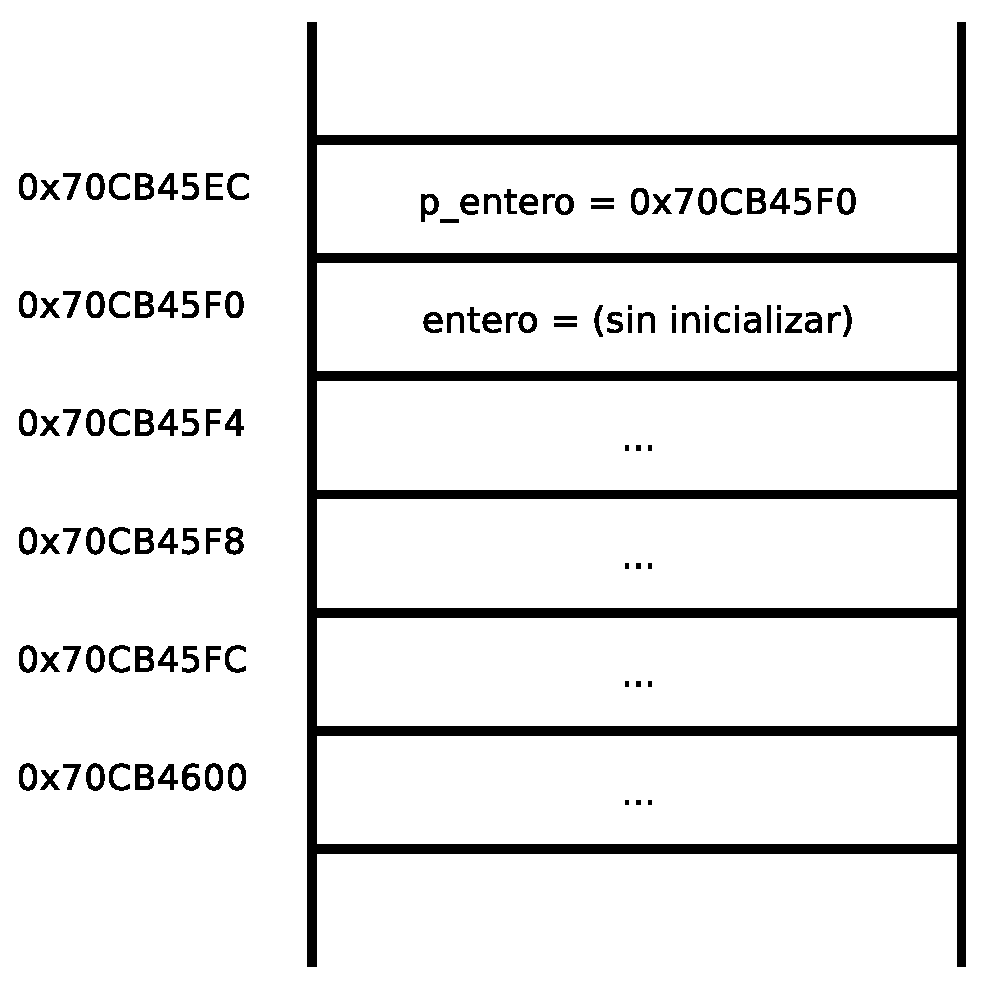
\includegraphics[width=80mm]{punteros/images/init_punteros.eps}
\caption{Inicializando punteros}
\end{centering}
\end{figure}

El operador \texttt{*} se utilizar para manejar la direcci�n a la que
apunta un puntero. Podr�amos llamarlo el operador de
\textit{acceso}. Tanto el operador de acceso, como el de indirecci�n,
funcionan en \textbf{notaci�n prefija}. Veamos un ejemplo que combina
ambos operadores:

\begin{verbatim}
1 int *p_entero;
2 int entero1, entero2;
3 entero1 = 2;
4 entero2 = 5;
5 p_entero = &entero1;
6 entero1 = *p_entero + entero2;
\end{verbatim}

Del mismo modo podemos asignar un valor a la variable a la que apunta
el puntero, de la forma:

\begin{verbatim}
1 int *p_entero;
2 int entero1, entero2;
3 entero1 = 2;
4 entero2 = 5;
5 p_entero = &entero1;
6 *p_entero = entero1 + entero2;
\end{verbatim}

Este �ltimo c�digo ejecutar�a \textbf{exactamente} lo mismo que el
anterior. Debemos notar que no tendr�a sentido prescindir de la linea
5, puesto que estar�amos intentando introducir el valor
\texttt{entero1 + entero2} en una direcci�n de memoria que no
conocemos, puesto que no le habriamos dado valor a \texttt{p\_entero}
(ver \ref{punteros_roma}).


%%
%% STRINGS (ana)
%%

%% SECCI�N: STRINGS  (autor: ana)

\section{Strings}
\label{strings}

Los arrays de caracteres se llaman \textbf{strings}. Funcionan
exactamente igual que cualquier otro array.  En los \textbf{strings}
no hace falta una variable que guarde el tama�o del array, puesto que
se marca el final del array con el car�cter ``\verb+\0+''.  La ventaja de los
\textbf{strings} es que podemos rellenar y consultar varios elementos
del array a la vez. En lugar de:

\begin{verbatim}
cadena[0] = 'h';
cadena[1] = 'o';
cadena[2] = 'l';
cadena[3] = 'a';
cadena[4] = '\0';
\end{verbatim}

Podremos hacer esto:

\begin{verbatim}
cadena = "hola";
/* cuando metemos un texto entre comillas dobles, al copiarlo al array
   el car�cter '\0' se incluye solo. */
print ("%s",cadena);
\end{verbatim}

Una serie de fallos comunes al trabajar con strings se exponen en
\ref{error_considerar_puntero}.\\

Existen funciones espec�ficas para trabajar con strings
(\verb+#include <string.h>+) para realizar ese tipo de
tareas. Recomendamos al lector que consulte la documentaci�n de
funciones como \textit{strlen, strcpy, strncpy, strdup, strcat}.


%%
%% ARITMETICA (jorge)
%%

%% SECCI�N: ARITMETICA DE PUNTEROS (autor: jorge)
\section{Aritm�tica de punteros}
\label{punteros_aritmetica}

Es posible realizar operaciones aritm�ticas sobre las variables de
tipo puntero para conseguir que apunten a una posici�n diferente.
Por ejemplo:

\begin{verbatim}

char cadena[5];
char *puntero;

puntero = &cadena[0]; /* puntero apunta a cadena[0] */
*puntero = 'h';       /* cadena[0] = 'h' */
*(puntero+1) = 'o';   /* cadena[1] = 'o' */
*(puntero+2) = 'l';   /* cadena[2] = 'l' */
*(puntero+3) = 'a';   /* cadena[3] = 'a' */
*(puntero+4) = '\0';  /* cadena[4] = '\0' */

\end{verbatim}

\begin{figure}[H]
\begin{centering}
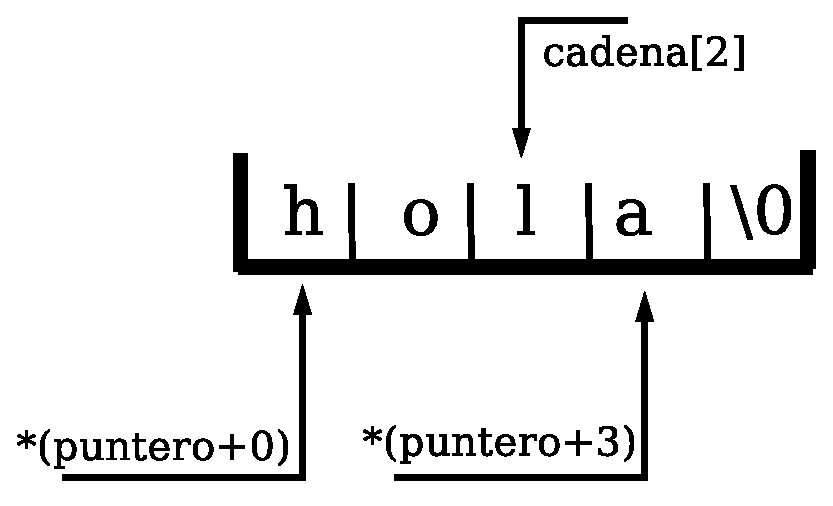
\includegraphics[width=70mm]{punteros/images/aritmetica0.eps}
\caption{Aritm�tica sobre un puntero}
\end{centering}
\end{figure}

\subsection{Contexto}

Se debe tener en cuenta que \verb-puntero+x- apuntar� a la direcci�n
de puntero sum�ndole \verb+x+ veces el espacio ocupado por un elemento
del tipo al que apunta, no el n�mero de bytes. 

\begin{figure}[H]
\begin{centering}
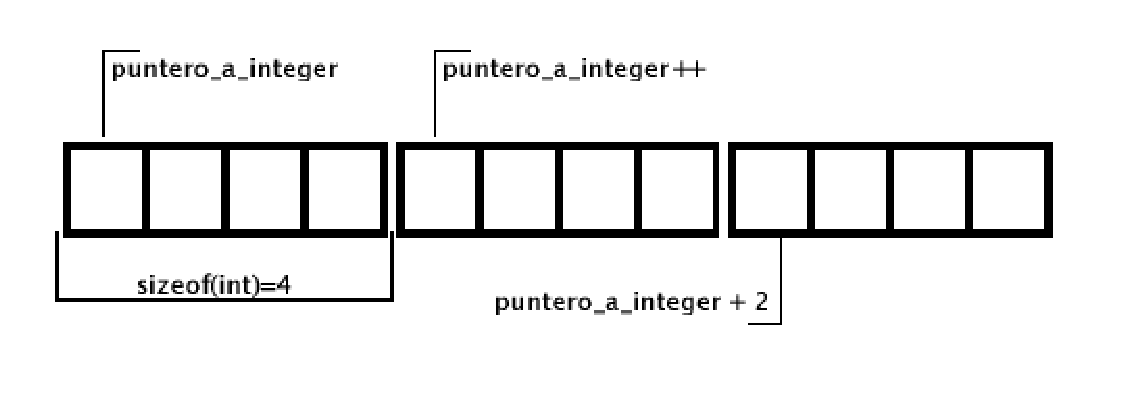
\includegraphics[width=130mm]{punteros/images/aritmetica1.eps}
\caption{Suma sobre un puntero a integer}
\end{centering}
\end{figure}

El programa mostrado a continuaci�n nos muestra la diferencia entre
considerar un puntero a integer y un puntero a char, en lo que se
refiere a la suma: 

\ejemplo{punteros/aritmetica/ejemplo_arit_punteros.c}

El resultado de ejecutar 
\footnote{Una vez m�s, recordamos que el tama�o de las variables en C
  es dependiente de la plataforma sobre la que compilemos/ejecutemos}
el c�digo anterior es:

\begin{verbatim}
Tama�o de int: 4
Tama�o de char: 1
Distancia entre punteros sucesivos a int : 4
Distancia entre punteros sucesivos a char: 1
\end{verbatim}

Queda clara la importancia entre declarar un puntero de un tipo o
otro. Ambos punteros del ejemplo ocupan lo mismo, ambos apuntan a
direcciones de memoria del sistema, pero cuando el compilador tiene
que generar c�digo para realizar operaciones aritm�ticas, lo hace de
manera distinta en funci�n del tipo de puntero.

\subsection{Tipos de operaciones}

Las operaciones soportadas sobre punteros son:

\begin{itemize}

\item Suma y resta de valores enteros ($+$,$-$,$++$ y $--$)
\item Comparaci�n y relaci�n ($<$,$>$,$<=$,$>=$,$==$ y $!=$)
\item Valor booleano (comparaci�n con NULL)

\end{itemize}

\subsection{Ejemplos de aritm�tica}

A continuaci�n mostramos un ejemplo de una funci�n que recibe dos
strings (ver \ref{strings}), y copia uno sobre otro. En la segunda
versi�n, las operaciones de aritm�tica de punteros se han agrupado,
para escribir menos c�digo. La finalidad de la segunda versi�n es
acostumbrar al lector a la complejidad de algunas operaciones en C
(funci�n \textit{copiar}).\\

Primera versi�n: 

\ejemplo{punteros/aritmetica/ejemplo_suma_punteros.c}

Segunda versi�n:

\ejemplo{punteros/aritmetica/ejemplo_suma_punteros_dificil.c}

Comentaremos la siguiente sentencia:

\begin{verbatim}
  while(*dest++ = *orig++); 
\end{verbatim}

Para entender la sentencia, la observaremos desde el punto de vista de la
precedencia entre operadores. En primer lugar, se ejecutar�an los
post-incrementos, pero su efecto s�lo tendr�a lugar al acabar la
sentencia (la expresi�n parentizada). Por tanto, lo siguiente en
ejecutarse ser�a el operador de acceso (``*''). Eso acceder�a a los
caracteres apuntados por \verb+dest+ y por \verb+orig+. Despu�s se ejecutar�a la
asignaci�n, (copia de un car�cter de la cadena). Como se vi� en
\ref{operador_asignacion}, la asignaci�n ``devuelve'' el valor
asignado, por lo que la expresi�n parentizada equivale al valor que se
asigna. Cuando se asigna el �ltimo car�cter de la cadena (\verb+\0+),
el valor de la expresi�n es falso (\verb+\0+ equivale a 0, esto es,
falso), y el  \verb+while+ saldr�a. Antes de terminar de procesar, se
incrementar�an ambos punteros (post-incrementos), haciendo que apunten
al siguiente car�cter de la cadena.

\consejo{Normalmente el uso de la aritm�tica de punteros se centra en
operaciones sencillas de incremento o decremento.  Operaciones m�s
complejas son potencialmente peligrosas, adem�s operaciones como la
multiplicaci�n o divisi�n de dos apuntadores no estan permitidas lo
cual es bastante l�gico debido a la m�nima utilidad pr�ctica de estos
operadores en punteros. A la hora de programar se debe recordar que
un mal uso de la aritm�tica de punteros puede dejar poco portable 
nuestro c�digo.}



%%
%% STRUCTS Y PUNTEROS (ferda)
%%

%% SECCI�N: ESTRUCTURAS Y PUNTEROS
\section{Estructuras y punteros}

\subsection{El operador ``\texttt{->}''}
\label{operador_puntero_structs}

En programas un poco m�s elaborados, usaremos a menudo los punteros
para apuntar a estructuras (\texttt{struct}). Nada nos impide
referirnos a los campos de la estructura a la que apunta el puntero de
la forma que hemos visto hasta ahora, es decir, llamando al campo que
deseemos del contenido del puntero dado. Con este ejemplo entenderemos
mejor a qu� nos referimos:

\begin{verbatim}
struct coordenada {
   int x, y;
} coord;
struct coordenada *p_coord;
p_coord = &coord;
(*p_coord).x = 4;
(*p_coord).y = 3;
\end{verbatim}

\begin{flushleft}
Aun as� esto puede resultar algo engorroso, por eso C nos da la
posibilidad de usar el operador \texttt{->} que nos facilita las
cosas:
\end{flushleft}

\begin{verbatim}
struct coordenada {
   int x, y;
} coord;
struct coordenada *p_coord;
p_coord = &coord;
p_coord->x = 4;
p_coord->y = 3;
\end{verbatim}

Los dos c�digos anteriores ejecutan lo mismo pero en el segundo
utilizamos el operador \texttt{->}, que nos hace el c�digo m�s
legible. 

\nota{Es un error frecuente utilizar el operador punto sobre un
puntero a estructura.}  
 

%%
%% MEMORIA DINAMICA (mustang)
%%

%% SECCI�N: MEMORIA DIN�MICA (autor: mustang)

\section{Memoria din�mica}

\label{mem_dinamica}

\subsection{�Qu� es la memoria din�mica?}

Supongamos que nuestro programa debe manipular estructuras de datos de
longitud desconocida. Un ejemplo simple podr�a ser el de un programa
que lee las l�neas de un archivo y las ordena. Por tanto, deberemos
leer un n�mero indeterminado de l�neas, y tras leer la �ltima,
ordenarlas. Una manera de manejar ese ``n�mero indeterminado'', ser�a
declarar una constante \verb+MAX_LINEAS+, darle un valor
vergonzosamente grande, y declarar un array de tama�o
\verb+MAX_LINEAS+. Esto, obviamente, es muy ineficiente (y
feo). Nuestro programa no s�lo quedar�a limitado por ese valor m�ximo,
sino que adem�s gastar�a esa enorme cantidad de memoria para procesar
hasta el m�s peque�o de los ficheros.\\

La soluci�n consiste en utilizar memoria din�mica. La memoria din�mica
es un espacio de almacenamiento que se solicita \textit{en tiempo de
ejecuci�n}\footnote{cuando el programa llega al punto en el que
necesita espacio para una l�nea m�s}. De esa manera, a medida que el
proceso va necesitando espacio para m�s l�neas, va solicitando m�s
memoria al sistema operativo para guardarlas. El medio para manejar la
memoria que otorga el sistema operativo, es el puntero, puesto que no
podemos saber \textit{en tiempo de compilaci�n}\footnote{es decir, al programar}
d�nde nos dar� huecos el sistema operativo (en la memoria de nuestro
PC). 

\subsection{El mapa de memoria en Unix}

Antes de profundizar en el manejo de memoria din�mica, vamos a dar una
breve visi�n del mapa de memoria en Unix, esto es, c�mo se organiza la
memoria de un proceso. Ante todo, esto es una simplificaci�n, para
poder situar mejor los punteros en su contexto.\\

De entre las varias regiones de memoria que existen, hay dos que nos
interesan al hablar de punteros (y sobre todo, al depurar): la pila y
el heap. 

\subsubsection{La pila}

En ingl�s, stack. Su contenido se estudia en profundidad en las
asignaturas de \textit{Laboratorio de Estructura de Computadores} y
\textit{Compiladores}. Aqu� solo diremos que cada vez que se realiza
una llamada a una funci�n, se introduce en la pila una estructura que
almacena los par�metros pasados a la funci�n, y las variables
declaradas dentro de ella. Cuando la funci�n retorna, dicha estructura
es destruida. 

\subsubsection{El heap}

Esta regi�n queda disponible para las solicitudes de memoria din�mica
al sistema operativo. Su crecimiento va ligado a la disminuci�n de la
pila, y viceversa. 

\begin{figure}[H]
\begin{centering}
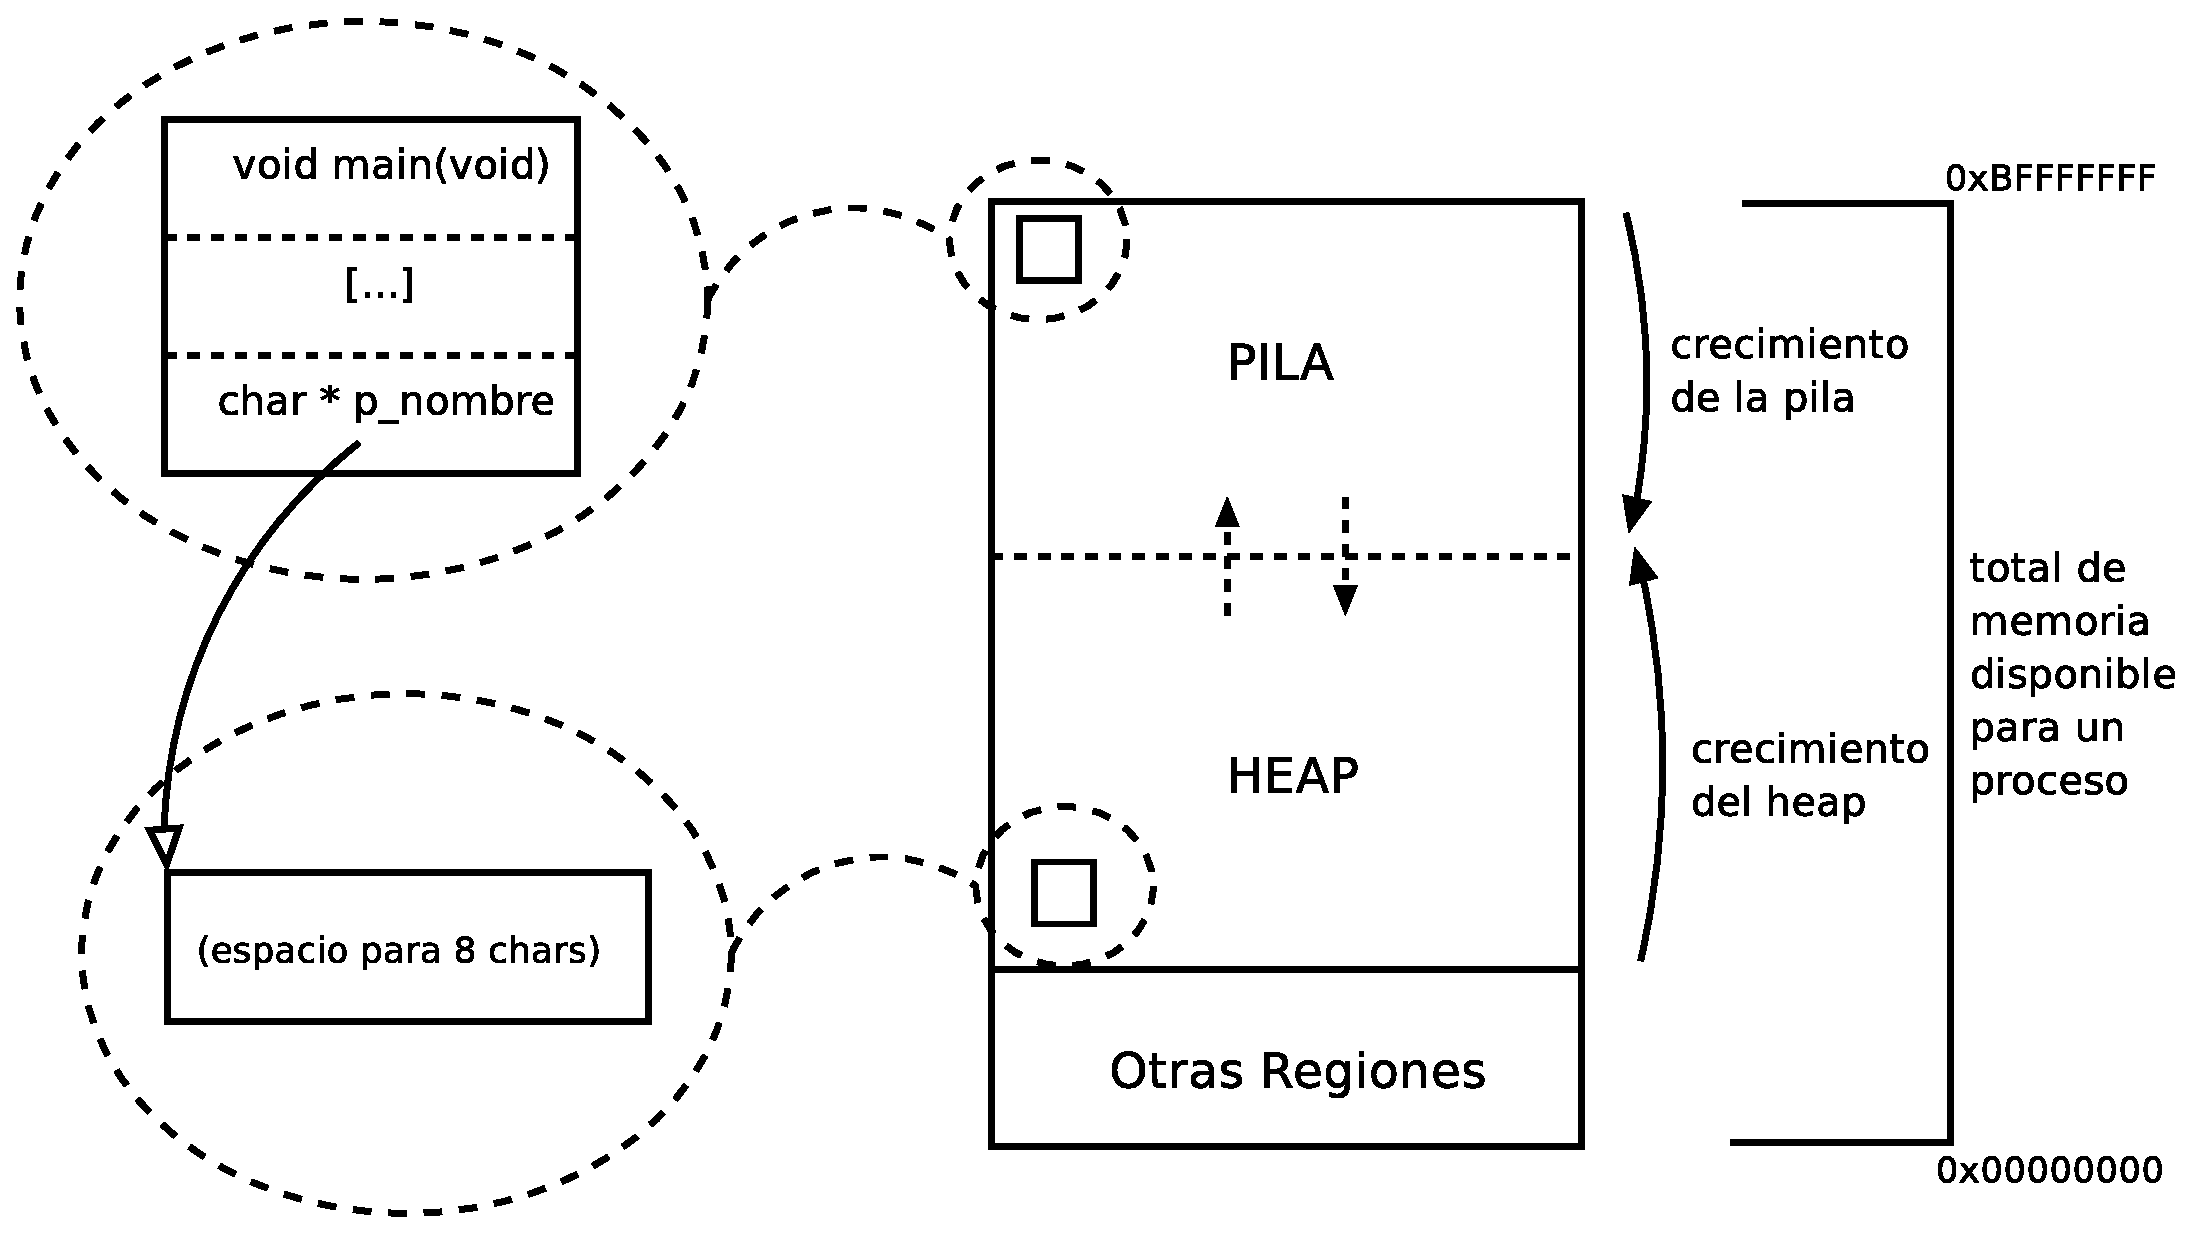
\includegraphics[width=145mm]{punteros/images/pila_heap.eps}
\caption{Visi�n general del mapa de memoria}
\end{centering}
\end{figure}

La figura anterior, muestra el resultado de solicitar al sistema
operativo espacio en memoria din�mica para 8 chars. Podemos quedarnos
con la idea de que las variables locales de una funci�n, y los
argumentos de la misma van en la pila, mientras que la memoria
din�mica va en el heap.

\subsection{Primitivas b�sicas}

Las primitivas b�sicas para el manejo de memoria din�mica son: 

\begin{itemize}
\item \verb+malloc+
\item \verb+realloc+
\item \verb+free+
\end{itemize}

\subsubsection{\texttt{malloc}}

Solicita memoria din�mica al sistema operativo. Su prototipo es:

\begin{verbatim}
void *malloc(size_t size);
\end{verbatim}

Devuelve un puntero tipo void, que apunta a la zona solicitada, o
NULL, en caso de no poderse cumplir la solicitud (probablemente por
falta de memoria libre). El tipo \verb+size_t+, tiene conversi�n
directa desde los \verb+int+.\\

Por ejemplo, si quisi�ramos solicitar memoria din�mica para almacenar
8 chars:

\begin{verbatim} 
char *p_char;
p_char = malloc(8*sizeof(char));
\end{verbatim}

No obstante, el autor prefiere especificar a mano los cast (ver
\ref{cast}) que se deben realizar para que encajen los argumentos:

\begin{verbatim} 
char *p_char;
p_char = (char *) malloc( (size_t) 8*sizeof(char));
\end{verbatim}

\nota{La zona de memoria devuelta por \texttt{malloc} no se inicializa a
  ning�n valor concreto.}

\subsubsection{\texttt{realloc}}

Cambia el tama�o de una zona de memoria din�mica, pedida al sistema
operativo previamente mediante la orden \verb+malloc+. Su prototipo es: 

\begin{verbatim}
void *realloc(void *ptr, size_t size);
\end{verbatim}

\begin{flushleft}
Un ejemplo de uso de \verb+realloc+:
\end{flushleft}

\begin{verbatim}
char *p_char;
int size;

size = 8 * sizeof(char);

/* pedimos memoria en p_char */
p_char = (char *) malloc( (size_t) size); 

[.....]

/* necesitamos m�s memoria en p_char */
size *= 2;
p_char = (char *) realloc(p_char, (size_t) size);
\end{verbatim}

\begin{flushleft}
Un ejemplo habitual de uso de \texttt{realloc} est� en
\ref{ejemplo_realloc_duro}. 
\end{flushleft}

\nota{\texttt{realloc} puede devolvernos la zona de memoria solicitada
  en otra posici�n. Esto es, independientemente de encargarse de
  reservar el nuevo espacio solicitado, el puntero que retorna \texttt{realloc}
  puede ser distinto al devuelto originalmente por \texttt{malloc}. Aun as�,
  \texttt{realloc} se encarga de que el contenido apuntado por el puntero sea
  el mismo. Dicho de otra manera, si pedimos memoria para x
  caracteres, y luego hacemos \texttt{realloc} sobre esa zona pidiendo x+n
  caracteres, \texttt{realloc} se encargar� de que los x primeros caracteres de
  la zona devuelta (sea la misma zona pero m�s grande, o sea otra zona
  distinta) sean id�nticos. Como es habitual, si solicitamos m�s
  espacio, ese espacio extra no ser� inicializado.}

\subsubsection{\texttt{free}}

Libera una zona de memoria din�mica, solicitada previamente mediante
\verb+malloc+. Su prototipo es: 

\begin{verbatim}
void free(void *ptr);
\end{verbatim}

\begin{flushleft}
Un ejemplo de uso de \texttt{free}:
\end{flushleft}

\begin{verbatim}


char *p_char;

/* pedimos memoria en p_char */
p_char = (char *) malloc( (size_t) 8*sizeof(char)); 

[...]

free(p_char);
\end{verbatim}

\nota{Liberar una zona de memoria una segunda vez es
  ilegal (ver \ref{error_doble_liberacion}).}

\nota{Es habitual al empezar a manejar memoria din�mica, dejar la
  tarea de liberar la memoria solicitada para el final. Esto es una
  mala pol�tica de trabajo. Por cada \texttt{malloc} que utilizamos, debemos
  pensar donde se va a hacer su \texttt{free}, y colocar ambos en el c�digo. En
  cuanto los programos crecen, es habitual olvidarse de liberar
  memoria, y el consumo de nuestros programas pueden crecer de manera
  desorbitada.}

\subsubsection{strdup}

Es una primitiva incluida en \textit{string.h}. La hemos incluido en
el manual, porque se usa frecuentemente, aunque al igual que strdup,
hay muchas llamadas al sistema similares (piden memoria din�mica por
nosotros). Su prototipo es:

\begin{verbatim}
  char *strdup(const char *s);
\end{verbatim}

Es una funci�n bastante c�moda, le suministramos un puntero a un
string, y nos devuelve un puntero a una zona de memoria din�mica, que
es una copia de la cadena que le hemos pasado. Dicho de otra manera,
strdup equivale a hacer un \texttt{malloc} de la longitud de la cadena
argumento, y a copiarla sobre la zona devuelta. Un ejemplo de uso ser�a:

\begin{verbatim}
char * pointer;
char * data = "Hello world\n";

pointer = strdup(data);

printf("%s", pointer);

free(pointer);
\end{verbatim}
%"

Este caso es un candidato ideal para mostrar un error frecuente al
trabajar con strings y punteros (ver
\ref{error_confundir_strings_punteros}).


%%
%% ARRAYS Y PUNTEROS (ana)
%%

%% SECCI�N: ARRAYS Y PUNTEROS  (autor: ana)
\section{Arrays y punteros}
\label{arrays_punteros}

\begin{flushleft}
Hasta ahora para nosotros un array era un conjunto ordenado de
elementos del mismo tipo.
\end{flushleft}

\subsection{Repaso}

\begin{flushleft}
La sintaxis en C para declarar un array es:
\end{flushleft}

\begin{verbatim}
tipo_elementos nombre_array[numero_elementos];
\end{verbatim}

\begin{flushleft}
La sintaxis para acceder a sus elementos es:
\end{flushleft}

\begin{verbatim}
nombre_array[indice]
\end{verbatim}

\begin{flushleft}
Ejemplo: un array de cinco elementos que contenga n�meros primos ser�a as�:
\end{flushleft}

\begin{verbatim}
int numeros_primos[5];

numeros_primos[0] = 2;
numeros_primos[1] = 3;
numeros_primos[2] = 5;
numeros_primos[3] = 7;
numeros_primos[4] = 11;
\end{verbatim}

\subsection{Introducci�n}

Ahora vamos a ver qu� es para el compilador un array, y as�
aprenderemos a usarlos de manera m�s eficiente. Un array es un
conjunto de elementos del mismo tipo. Para que sea conjunto
``ordenado'', lo que el compilador hace es juntar todos los elementos
en la misma zona de memoria. Almacena la direcci�n inicial en nuestra
variable para saber d�nde est� el primer elemento, que corresponder�a
al �ndice ``0''. A partir de ah�, al incrementar la direcci�n de
memoria en el tama�o de los elementos, va accediento a array[1],
array[2], etc.

\begin{figure}[H]
\begin{centering}
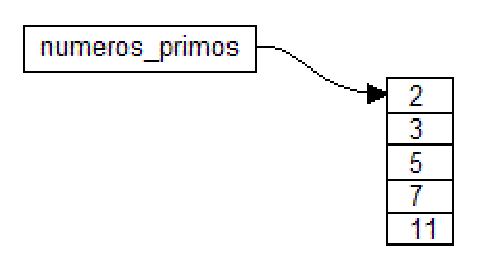
\includegraphics[width=65mm]{punteros/images/arrays_1.eps}
\caption{Un array de n�meros primos}
\end{centering}
\end{figure}

\begin{figure}[H]
\begin{centering}
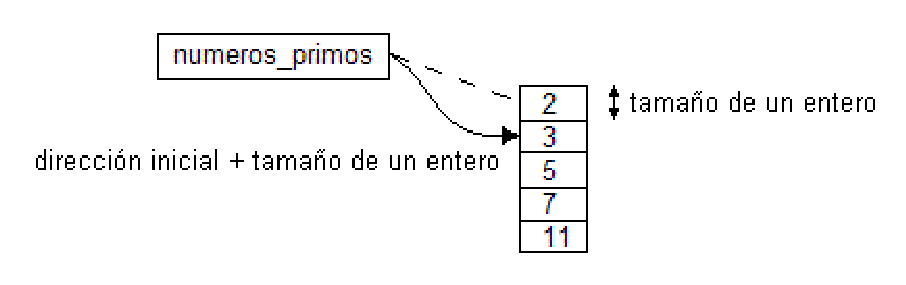
\includegraphics[width=115mm]{punteros/images/arrays_2.eps}
\caption{Avanzando sobre un array}
\end{centering}
\end{figure}

As� podemos deducir la siguiente f�rmula: 
\textit{direcci�n\_elemento$=$direcci�n\_inicial$+($�ndice$*$tama�o\_elementos$)$}.\\

Esta f�rmula es la que aplica el compilador para calcular la direcci�n
del elemento al que nos referimos al hacer un acceso al array del tipo
\textit{array[indice]}, como por ejemplo \textit{numeros\_primos[3]}.
Claramente, se dibuja la idea del puntero en el concepto de
array:\\

\definicion{Variable tipo array}{Un puntero al primer elemento del
array.}

�Cu�l es la ventaja de trabajar de punteros, con los posibles
problemas que eso trae, en vez de con arrays sin m�s?  La respuesta
surge enseguida: un array tiene un tama�o fijo desde su
declaraci�n. Sin embargo, trabajando con punteros, nuestro array podr�
tener el tama�o que nosotros queramos durante el programa, y podemos
incluso variarlo en funci�n de otros datos del programa.\\

Por supuesto, esta ventaja tiene un precio (aunque muy bajo) que no
debemos olvidar. Debemos apuntar en alg�n sitio (variable, constante)
cu�nto espacio hemos pedido y en otro cu�nto de ese espacio hemos
aprovechado. Como al programar no conoceremos el espacio aprovechado
del array, deberemos hacer una de estas dos cosas:

\begin{itemize}
\item apuntar en otra variable el tama�o ocupado del array.  
\item hacer que el �ltimo elemento del array sea diferente, un dato
  que no nos puedan introducir, por ejemplo, un n�mero negativo o una letra cuando hablamos
  de n�meros de tel�fono. 
\end{itemize}

\begin{figure}[H]
\begin{centering}
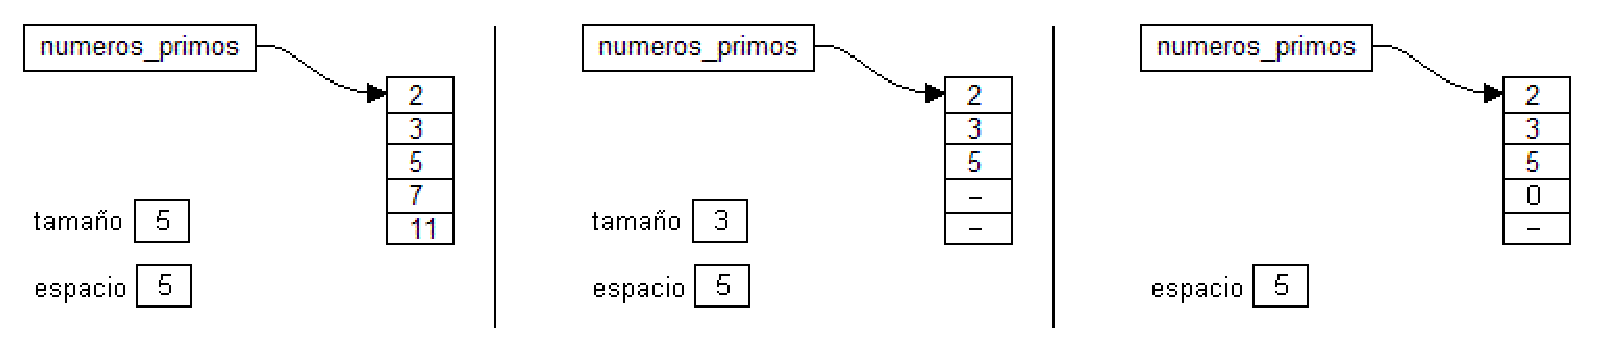
\includegraphics[width=170mm]{punteros/images/arrays_3.eps}
\caption{M�s sobre arrays}
\end{centering}
\end{figure}

\paragraph{Ejemplo}
Queremos que el usuario introduzca varios n�meros de tel�fono y los
vamos a almacenar en el array \textit{telefonos}. No sabemos cu�ntos
n�meros va a introducir el usuario. Si lo tuvi�ramos que implementar
con un array definido desde su
declaraci�n, tendr�amos que poner un tope a los n�meros de tel�fono
que se pueden introducir, por ejemplo 10:

\begin{verbatim}
int i;
int telefonos[10];

i=0;
while (usuario_introduce && (i<10))
{
  telefonos[i] = numero_introducido;
  i++;
}
numeros_introducidos = i;
\end{verbatim}

Sin embargo, trabajando con punteros podemos preguntar al usuario
cu�ntos n�meros quiere introducir:

\begin{verbatim}
int i, tamano;
int *telefonos; // o bien: int telefonos[]

telefonos = NULL;
/* es muy recomendable inicializar el valor de un puntero a NULL.
 * As�, si se nos olvida pedir memoria para �l, el programa fallar� siempre.
 * Por el contrario, si no lo inicializamos, el programa fallar� 
 * algunas veces s� y otras no. */

tamano = preguntar_tamano();
telefonos = malloc (tamano);

for (i=0;i<tamano;i++)
  telefonos[i] = numero_introducido;
\end{verbatim}

O tambi�n variar el tama�o del array de forma din�mica:

\begin{verbatim}

int i, tamano, nuevo_tamano;
int *telefonos; // o bien: int telefonos[]

telefonos = NULL;
i=0;
while (usuario_introduce)
{
  nuevo_tamano = sizeof (int) * (i+1);
  telefonos = realloc (telefonos,nuevo_tamano);
  telefonos[i] = numero_introducido;
  i++;
}
tamano=i;
\end{verbatim}

\nota{Si el tama�o del array es ``X'', los �ndices (que empiezan por cero) ir�n de ``0'' a ``X-1''.}



%%
%% INDIRECCIONES MULTIPLES (luisc)
%%

%% SECCI�N: INDIRECCIONES M�LTIPLES
\section{Indirecciones m�ltiples}

Una herramienta muy �til que proporciona C en su manejo de punteros
son las indirecciones m�ltiples, es decir, punteros que apuntan a
punteros. Las indirecciones pueden ser dobles, triples, cuadruples \dots.

\subsection{Declaraci�n}

Ejemplo:

\begin{verbatim}
char **ind_doble;
char ***ind_triple;
\end{verbatim}

La primera declaraci�n declarar�a un puntero de indirecci�n doble de
tipo char (l�ase: puntero que apunta a puntero), mientras que la
segunda declarar�a un puntero de indirecci�n triple a char (puntero
que apunta un puntero que apunta a otro puntero [es decir, un
l�o]). Usar m�s de indirecci�n triple es abiertamente desaconsejable.

\begin{figure}[H]
\begin{centering}
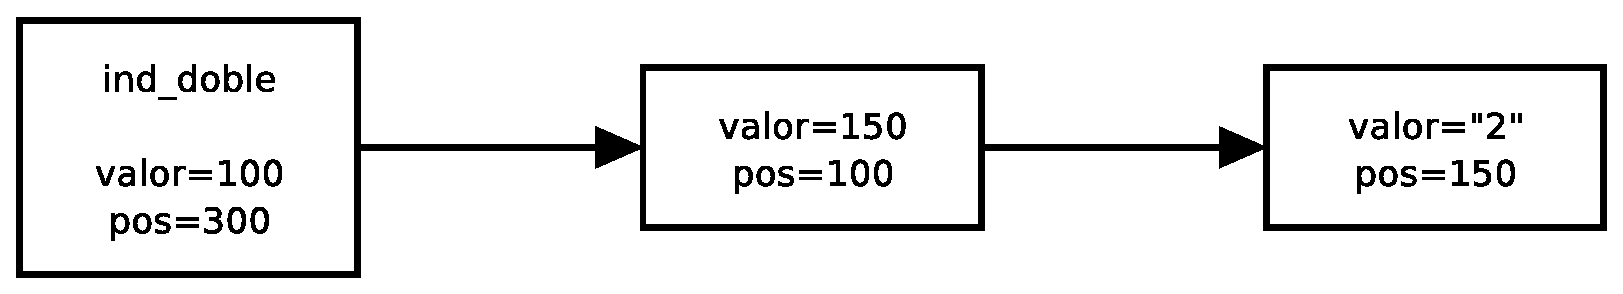
\includegraphics[width=110mm]{punteros/images/ind_doble.eps}
\caption{Indirecci�n doble}
\end{centering}
\end{figure}

\begin{figure}[H]
\begin{centering}
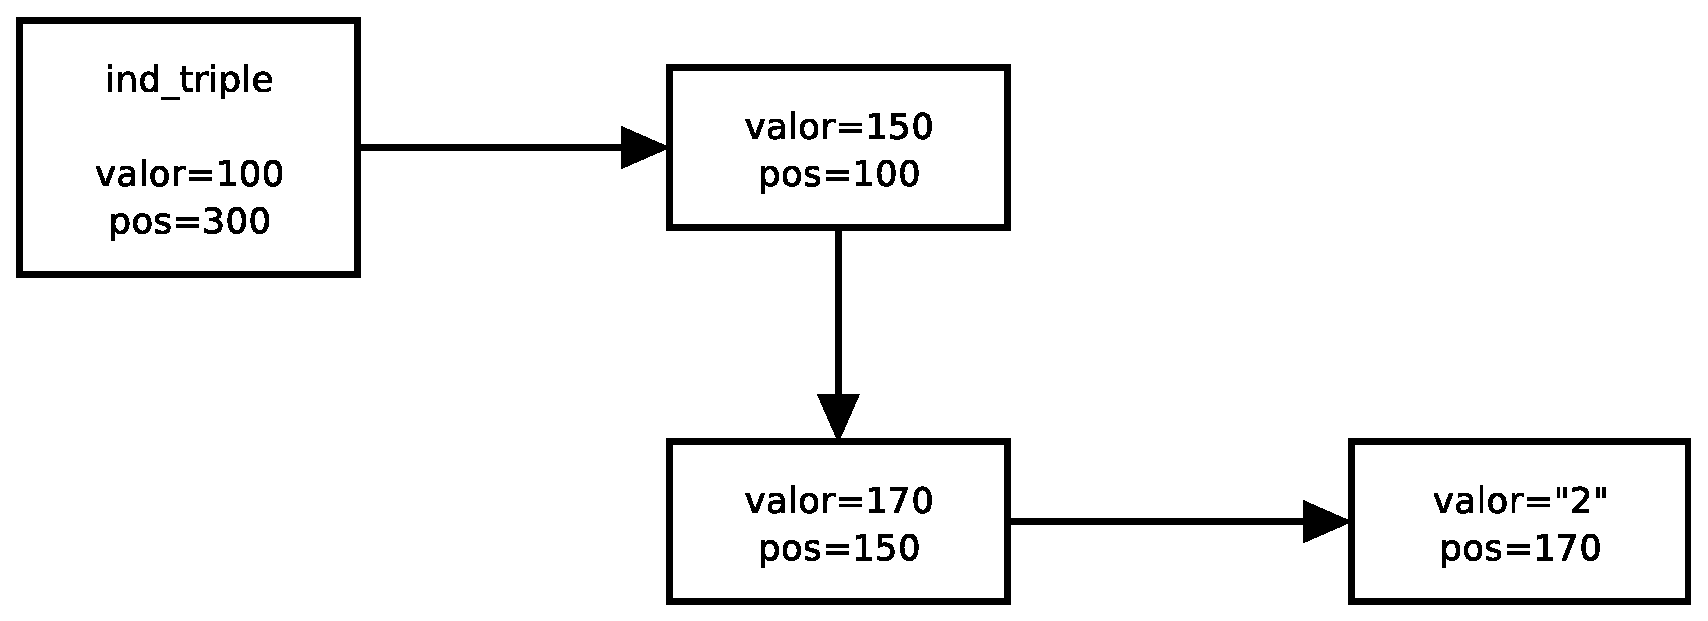
\includegraphics[width=110mm]{punteros/images/ind_triple.eps}
\caption{Indirecci�n triple}
\end{centering}
\end{figure}

\subsection{Utilizaci�n}

\begin{verbatim}
char **ind_doble;
char *puntero_normal;

/* Este acceso nos dar�a la direcci�n de la primera indirecci�n */

puntero_normal = *ind_doble;

/* Estos dos accesos ser�an equivalentes (despues de la asignaci�n de
 * arriba) */
 
*puntero_normal = 'A';
**ind_doble = 'A';
\end{verbatim}

Esto es as� porque \verb+*ind_doble+, es un puntero a char, es decir,
como regla cada \verb+*+ que pongamos en un puntero con indirecci�n
m�ltiple quitamos un nivel de indirecci�n.\\

Una vez m�s, recordar la dualidad entre �ndices de array y
punteros. Por ejemplo, cuando tratamos con un puntero de doble
indirecci�n, como puede ser \verb+char **data+, las expresiones
\begin{itemize}
\item\verb-data[1][2]- y 
\item \verb-*(*(data+1)+2)- 
\end{itemize}
son equivalentes.

\paragraph{Ejemplo}

\begin{itemize}
\item \verb+*ind_doble+ ser�a un puntero simple (de los vistos
  anteriormente).
\item \verb+**ind_doble+ ser�a el valor apuntado, es decir el
  car�cter de los ejemplos anteriores.
\item \verb+*ind_triple+ ser�a un puntero de indirecci�n doble.
\end{itemize}

\subsection{Ejemplos de uso}

Uno de los usos de punteros de indirecci�n m�ltiple, es, por ejemplo,
leer un texto completo y almacenarlo por l�neas.

\begin{verbatim}
char **texto;
\end{verbatim}

Cada \verb+*texto+ ser�a una l�nea, y cada \verb+**texto+ una letra de
la l�nea seleccionada. Ve�moslo con un programa:

\ejemplo{punteros/multiples/ejemplo_punteros_multiples.c}

\label{ejemplo_realloc_duro}
El siguiente ejemplo es especialmente interesante, combina el uso de
\verb-malloc- y \verb-realloc- con indirecciones m�ltiples. El programa utiliza un
doble puntero, sobre el que ejecuta un \verb-malloc-, y posteriormente, un
\verb-realloc- por cada nueva l�nea que vayamos leyendo. En cada nuevo
espacio que devuelve \verb-realloc-, se ejecuta un \verb-malloc- para almacenar una
nueva l�nea de texto.

\ejemplo{punteros/multiples/multiples_realloc.c}

Debemos tener en cuenta que el orden de los \verb-free- es importante:
primero liberamos cada uno de los \verb-malloc- que se ejecutaron dentro del
bucle (zonas sueltas de memoria, que almacenan una l�nea cada una). Al
final, liberamos el doble puntero, sobre el que hemos ejecutado un
\verb-malloc-, y varios \verb-realloc-. Si hici�ramos la liberaci�n al rev�s,
estar�amos pas�ndole como argumento a \verb-free-, punteros situados en una
zona de memoria que ha sido liberada (ya no es nuestra). El
comportamiento ser�a impredecible. \\

Como se vi� en la secci�n \ref{arrays_punteros}, es indiferente
acceder a un puntero m�ltiple usando la notaci�n de los arrays o el
operador de acceso junto con la aritm�tica de punteros:

\begin{verbatim}
double ** pointer;
double * p1;

p1 = (double *) malloc((size_t) 8 * sizeof(double));
pointer = &p1;  /* pointer apunta a p1 */

pointer[0][0]=3.141592;
pointer[0][1]=6.022E23;

printf("%g %g\n",pointer[0][0], pointer[0][1]);
printf("%g %g\n",**pointer, *(*pointer+1));
\end{verbatim}

\subsection{Cadenas enlazadas}

Uno de los usos m�s utiles de punteros es la implementaci�n de las
cadenas enlazadas, que se estudian en la asignatura de
\textit{Estructura de Datos I}.\\

El tipo \verb+cadena_enlazada+ es un puntero a un nodo, consistente de
un puntero al siguiente nodo (una cadena\_enlazada en si misma) y un
dato de un tipo cualquiera.\\

La dificultad de implementar es qu� tipo declarar primero, nodo o
cadena\_enlazada. Para ello, usaremos una t�cnica conocida como
\textit{forward declaration}. La idea consiste en avisar al compilador
de que estamos declarando un tipo, que es un puntero a una estructura,
pero que dicha estructura a�n no la hemos declarado, la declararemos
despu�s. 

\begin{figure}[H]
\begin{centering}
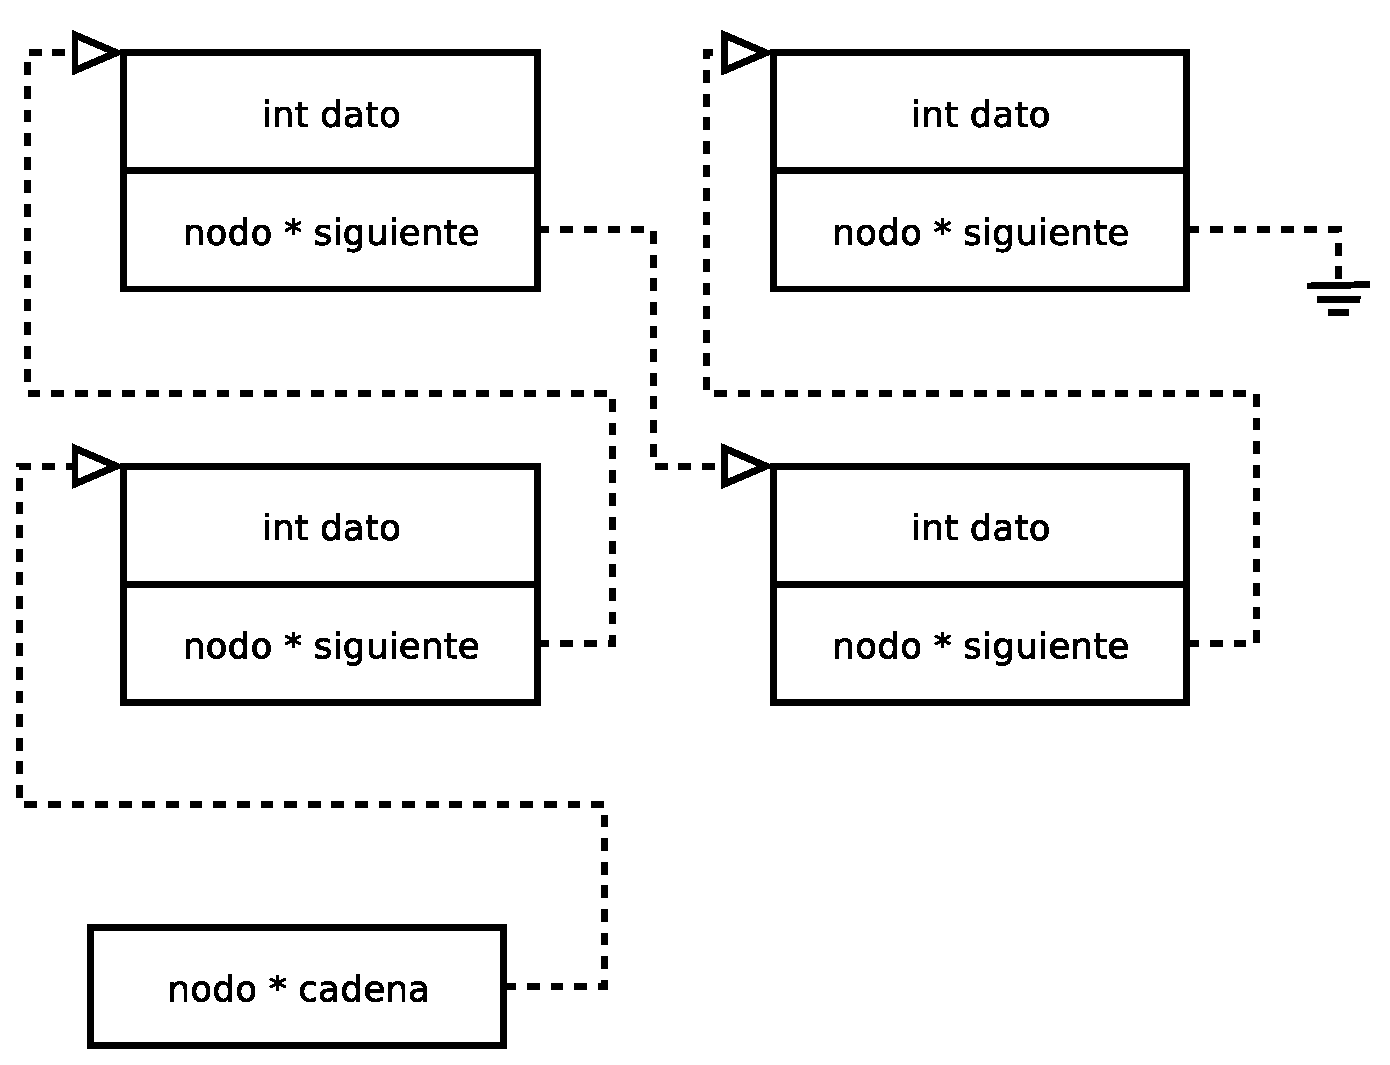
\includegraphics[width=100mm]{punteros/images/cadenas.eps}
\caption{Ejemplo de una cadena enlazada}
\end{centering}
\end{figure}

Una manera incorrecta de implementarlas ser�a:

\begin{verbatim}
typedef nodo * cadena_enlazada;

struct nodo{
  cadena_enlazada siguiente;
  int dato;
}
\end{verbatim}

debido a que el compilador no tiene definido el tipo \verb+nodo+ en el
momento de definir \verb+cadena_enlazada+. La forma correcta ser�a:

\begin{verbatim}
typedef struct nodo *cadena_enlazada;
        
struct nodo{
  cadena_enlazada siguiente;
  int dato;
};
\end{verbatim}

o tambi�n, si quisieramos realizar el \verb-typedef- sobre ambos tipos:

\begin{verbatim}
typedef struct nodo *cadena_enlazada;
        
typedef struct nodo{
  cadena_enlazada siguiente;
  int dato;
};
\end{verbatim}

Un ejemplo de uso de las cadenas enlazadas es:

\ejemplo{punteros/multiples/enl.c}



%%
%% PASO POR REFERENCIA vs PASO POR VALOR (cps)
%%

%% SECCI�N: PASO POR REFERENCIA vs PASO POR VALOR

\newpage

\section{Paso por referencia vs. paso por valor}

\label{valor_vs_referencia}

\subsection{�Qu� es el paso por referencia?}

A la hora de pasar una variable como argumento a una funci�n, el paso
por referencia consiste en entregar como argumento un puntero a la
variable, y no el contenido de la variable.

\subsection{�Para qu� necesito el paso por referencia?}

Si tratamos de modificar los valores de los argumentos de una funci�n, 
estos cambios no ser�n vistos desde fuera de la misma. Esto es debido
a que los argumentos de la funci�n son copias de las variables reales y
 son almacenadas como variables locales a dicha funci�n, desapareciendo 
por tanto al regresar a la llamante. Se incluye un ejemplo a continuaci�n:

\ejemplo{punteros/referencia_valor/no_mod_args.c}

Si compilamos y ejecutamos el c�digo anterior, obtenemos el 
siguiente resultado:
\begin{verbatim}
Variable var1 = 1
Variable var1 = 1
\end{verbatim}

Como era de esperar, no se ha modificado el valor de la variable \texttt{var1}
fuera de la funci�n.

Por esto, si queremos modificar el valor de un argumento en una funci�n,
debemos pasar este par�metro \textit{por referencia}, como se muestra
en el siguiente ejemplo:

\ejemplo{punteros/referencia_valor/mod_args.c}

Como se puede comprobar, la salida de este programa es correcta:
\begin{verbatim}
Variable var1 = 1
Variable var1 = 2
\end{verbatim}

Si en una funci�n quisi�ramos modificar un par�metro que fuera un puntero, 
ser�a necesario pasar como argumento la direcci�n del mismo, es decir, 
\textit{doble indirecci�n}. Y as� sucesivamente si el argumento fuera 
doble puntero, triple puntero, etc. \\

Tambi�n es muy aconsejable el paso por referencia en el caso en que una funci�n
reciba como argumento una gran estructura de datos (arrays, matrices, ...),
puesto que el paso por valor implicar�a una copia completa de la estructura
en el espacio de memoria de la funci�n.


%%
%% ERRORES CON PUNTEROS (cps)
%%

%% SECCI�N: ERRORES CON PUNTEROS

\section{Errores con punteros}

\subsection{Comparaci�n de punteros a cadenas}
\label{error_confundir_strings_punteros}

Un error que ocurre frecuentemente al empezar a programar en C 
es intentar comparar dos cadenas de caracteres mediante sus punteros.
Ve�moslo en el siguiente ejemplo:

\ejemplo{punteros/errores/strings.c}

En la ejecuci�n de este programa, tendr�amos la siguiente asignaci�n
de memoria:

\begin{figure}[H]
  \begin{center}
    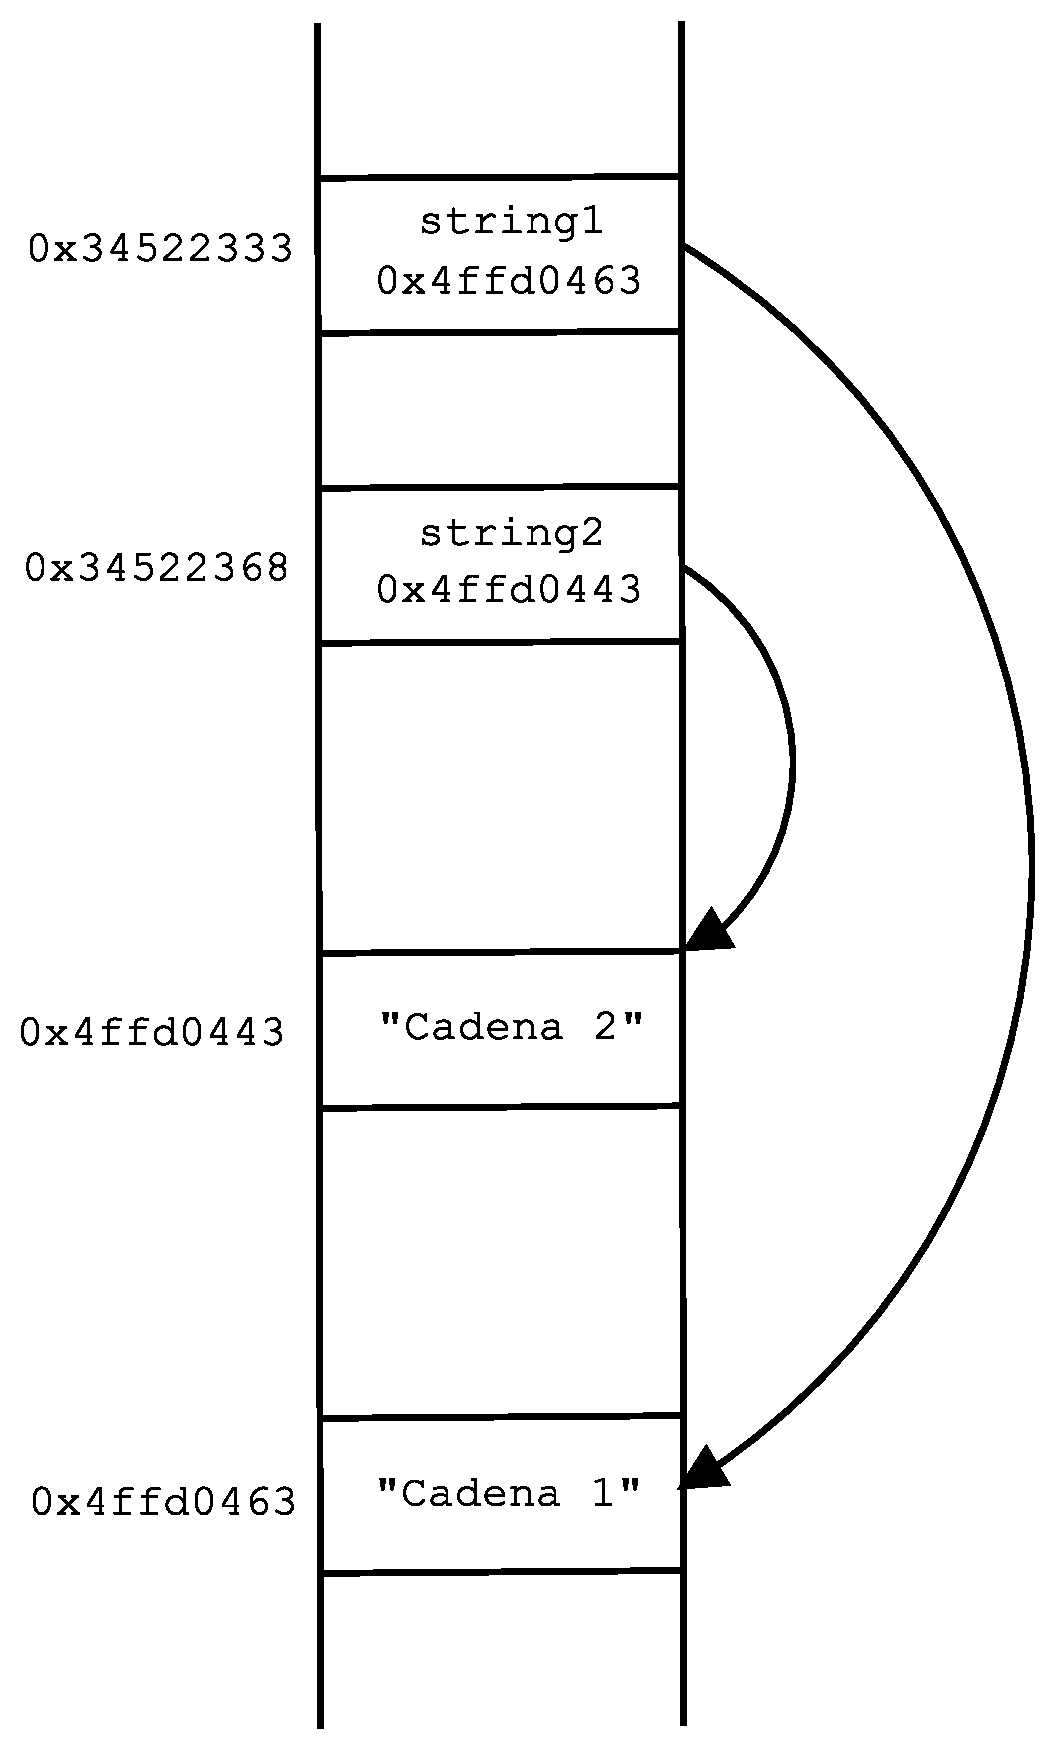
\includegraphics[height=9cm]{punteros/errores/strings.eps}
    \caption{Colocaci�n de strings en memoria}
  \end{center}
\end{figure}

Al observar el diagrama, se entiende m�s facilmente que el c�digo anterior 
no es correcto, esto es, �nicamente compara el valor de las variables
\texttt{string1} y \texttt{string2}, que son las direcciones de memoria
de las cadenas de caracteres, y no las cadenas en s�.\\

Por este motivo, si queremos comparar dos cadenas de caracteres correctamente,
deberemos usar las funciones de la librer�a est�ndar de C que operan sobre strings.
En concreto, la funci�n a utilizar es \texttt{strcmp}\footnote{Explicada m�s
 detalladamente en la secci�n \ref{strcmp}}, que compara dos cadenas 
car�cter a car�cter.\\

De esta manera, el c�digo corregido quedar�a:

\ejemplo{punteros/errores/strings_ok.c}

%%%%%%%%%%%%%%%%%%%%%%%%%%%%%%%%%%%%%%%%%%%%%%%%%%%%%%%%%%%%%%
%
%%%%%%%%%%%%%%%%%%%%%%%%%%%%%%%%%%%%%%%%%%%%%%%%%%%%%%%%%%%%%%

\subsection{Punteros ``a Roma"\ (\textit{memory leaks})}
\label{punteros_roma}

Observemos lo que ocurre en el siguiente ejemplo:
\ejemplo{punteros/errores/roma.c}

Al ejecutar el programa anterior, obtendr�amos el siguiente
diagrama:
\begin{figure}[H]
  \begin{center}
    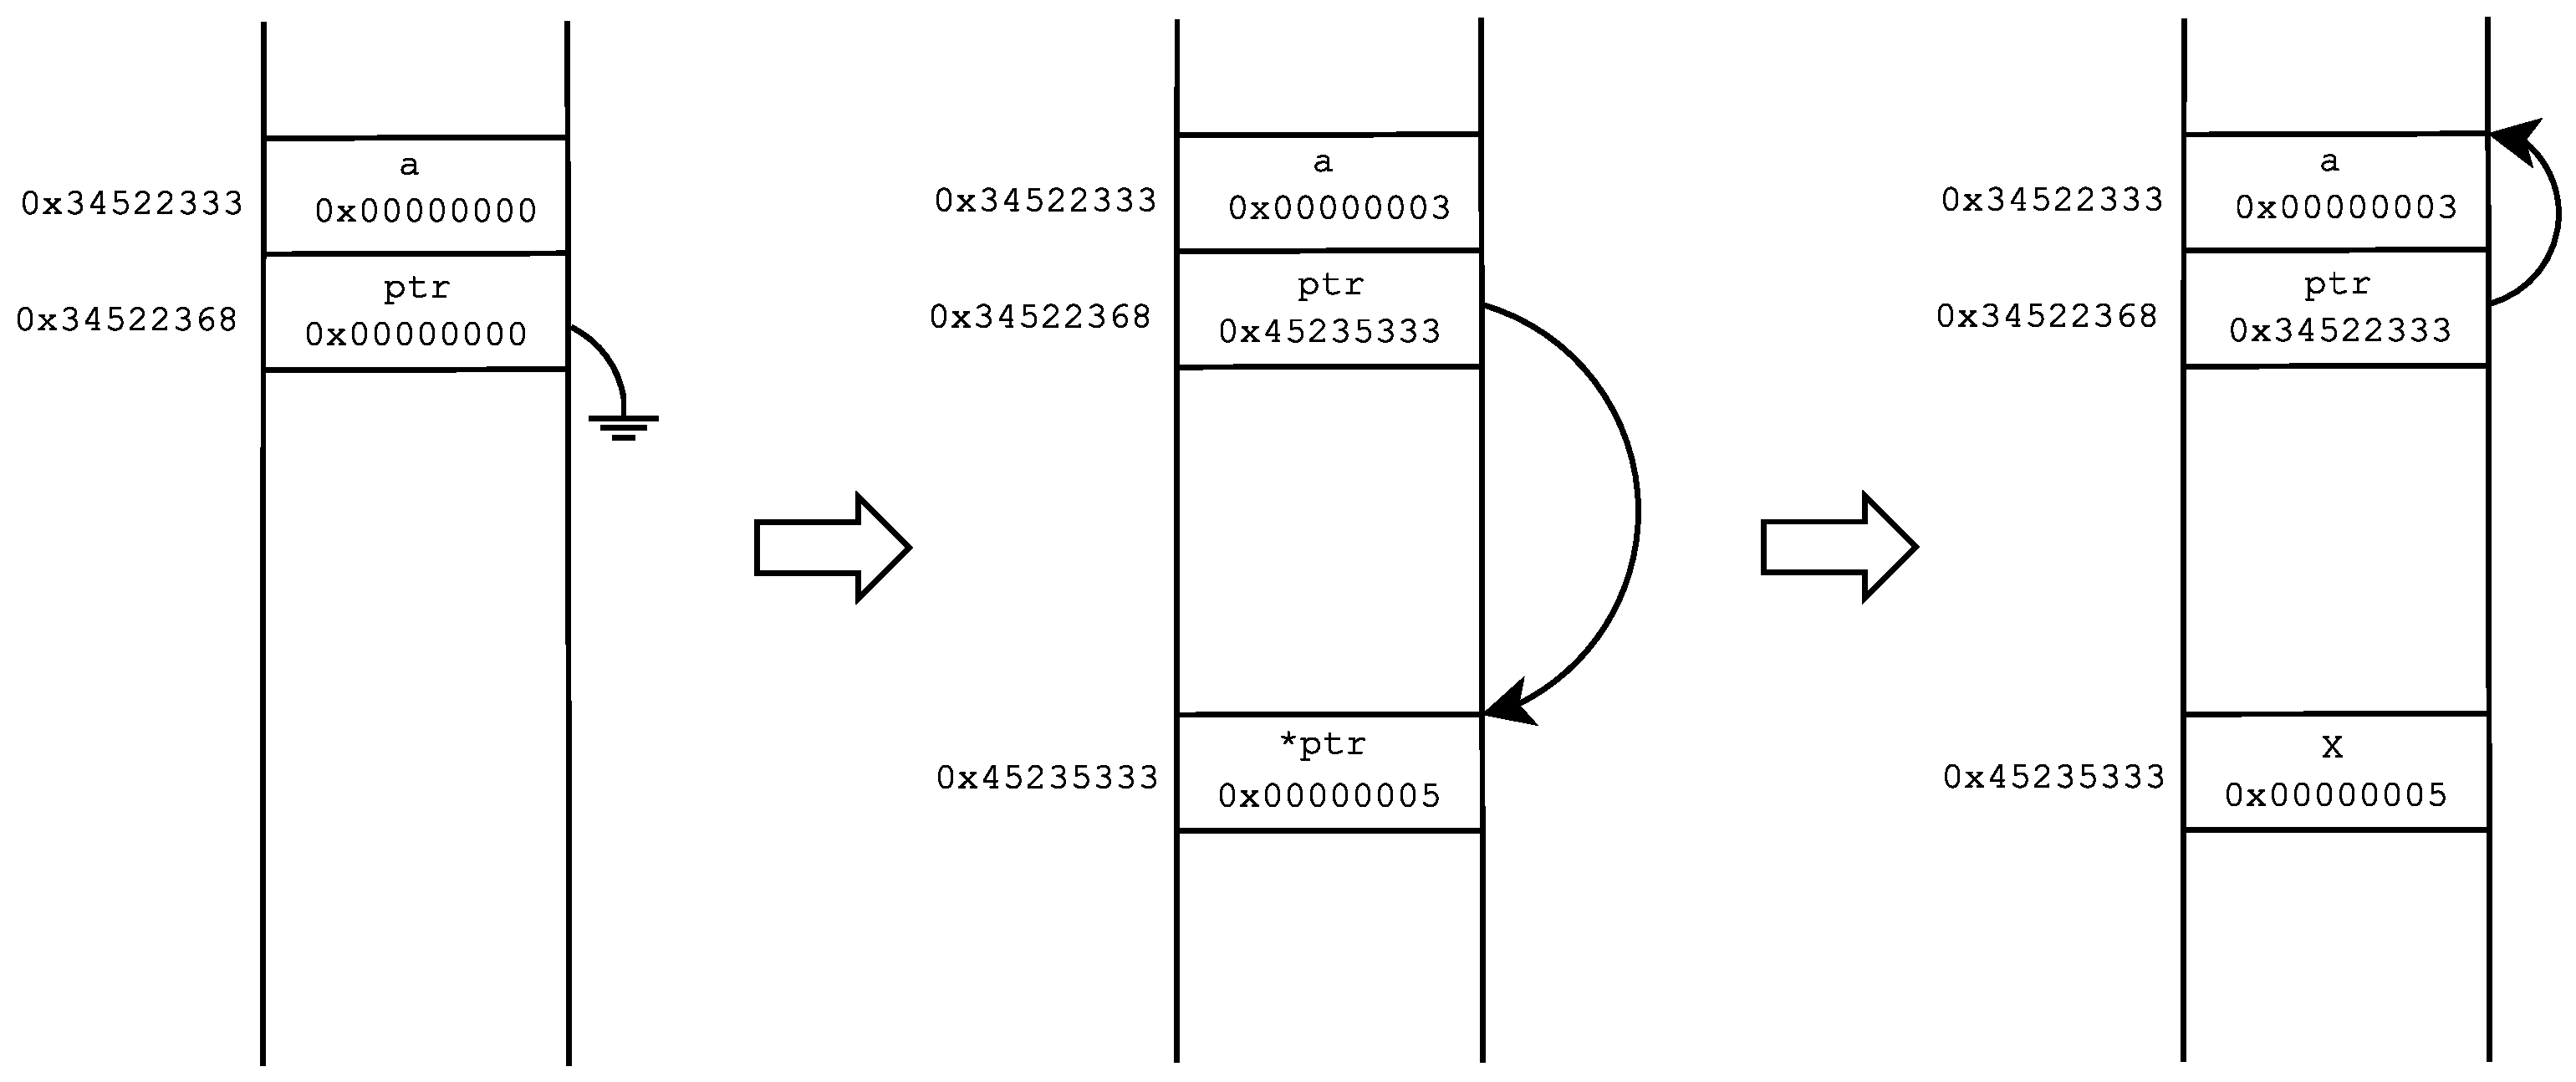
\includegraphics[width=14cm]{punteros/errores/roma.eps}
    \caption{Punteros a roma}
  \end{center}
\end{figure}

Como se puede apreciar, en la finalizaci�n del programa, ha quedado
una zona de memoria (\verb+0x45235333+) ocupada, que no esta apuntada
por ninguna variable. Esto implica no poder acceder al contenido
de dicha zona y por tanto, no poder liberarla, con el consiguiente
gasto innecesario de memoria.
%%%%%%%%%%%%%%%%%%%%%%%%%%%%%%%%%%%%%%%%%%%%%%%%%%%%%%%%%%%%%%
%
%%%%%%%%%%%%%%%%%%%%%%%%%%%%%%%%%%%%%%%%%%%%%%%%%%%%%%%%%%%%%%

\subsection{Doble liberaci�n}
\label{error_doble_liberacion}
Cuando se programa utilizando memoria din�mica, es necesario
liberar toda la memoria solicitada, pero �nicamente 
es necesario realizarlo una vez.
En ocasiones, se intenta liberar varias veces la misma zona de
memoria, consiguiendo un \texttt{Segmentation Fault}, pues
esta memoria ya estaba marcada como libre. Se puede comprobar con
un ejemplo muy simple como el siguiente:
\ejemplo{punteros/errores/mem.c}

%%%%%%%%%%%%%%%%%%%%%%%%%%%%%%%%%%%%%%%%%%%%%%%%%%%%%%%%%%%%%%
%
%%%%%%%%%%%%%%%%%%%%%%%%%%%%%%%%%%%%%%%%%%%%%%%%%%%%%%%%%%%%%%

\subsection{Usar $.$ en lugar de \texttt{->}}
Al utilizar estructuras apuntadas por punteros, hemos de tener
precauci�n y utilizar correctamente los operadores $.$ y \verb+->+
Vemos un mal uso de ellos en el siguiente ejemplo:

\ejemplo{punteros/errores/structs1.c}

%Y como se deber�a utilizar correctamente:
Y cual es su uso correcto:

\ejemplo{punteros/errores/structs2.c}


\label{error_considerar_puntero}


%%%%%%%%%%%%%%%%%%%%%%%%%%%%%%%%%%%%%%%%%%%%%%%%%%%%%%%%%%%%%%
%
%%%%%%%%%%%%%%%%%%%%%%%%%%%%%%%%%%%%%%%%%%%%%%%%%%%%%%%%%%%%%%

\subsection{Operar con los punteros en lugar de con los contenidos}
En los programas que utilizan punteros (memoria din�mica), es imprescindible
diferenciar perfectamente entre el puntero en s� y su contenido,
pues en otro caso, realizaremos algunas operaciones sobre el puntero
cuando en realidad queremos hacerlas sobre el contenido
\footnote{Un caso de este tipo es comentado m�s en detalle en
la secci�n \ref{error_confundir_strings_punteros}}. Veamos algunos errores m�s frecuentes:

\ejemplo{punteros/errores/contenido1.c}

Ahora la versi�n correcta:

\ejemplo{punteros/errores/contenido2.c}



%%%%%%%%%%%%%%%%%%%%%%%%%%%%%%%%%%%%%%%%%%%%%%%%%%%%%%%%%%%%%%
%
%%%%%%%%%%%%%%%%%%%%%%%%%%%%%%%%%%%%%%%%%%%%%%%%%%%%%%%%%%%%%%
\subsection{Finalizaci�n de cadenas}

En el lenguaje C, las cadenas de caracteres deben tener un
car�cter de finalizaci�n, \verb+\0+. Cuando asignamos
o inicializamos una variable con una cadena entre comillas dobles, el 
car�cter de finalizaci�n es puesto autom�ticamente por
el compilador, por ejemplo:

\begin{verbatim}
char * string1 = "Cadena";
\end{verbatim}

El c�digo anterior inicializar� la variable de la siguiente manera:
\begin{figure}[H]
  \begin{center}
    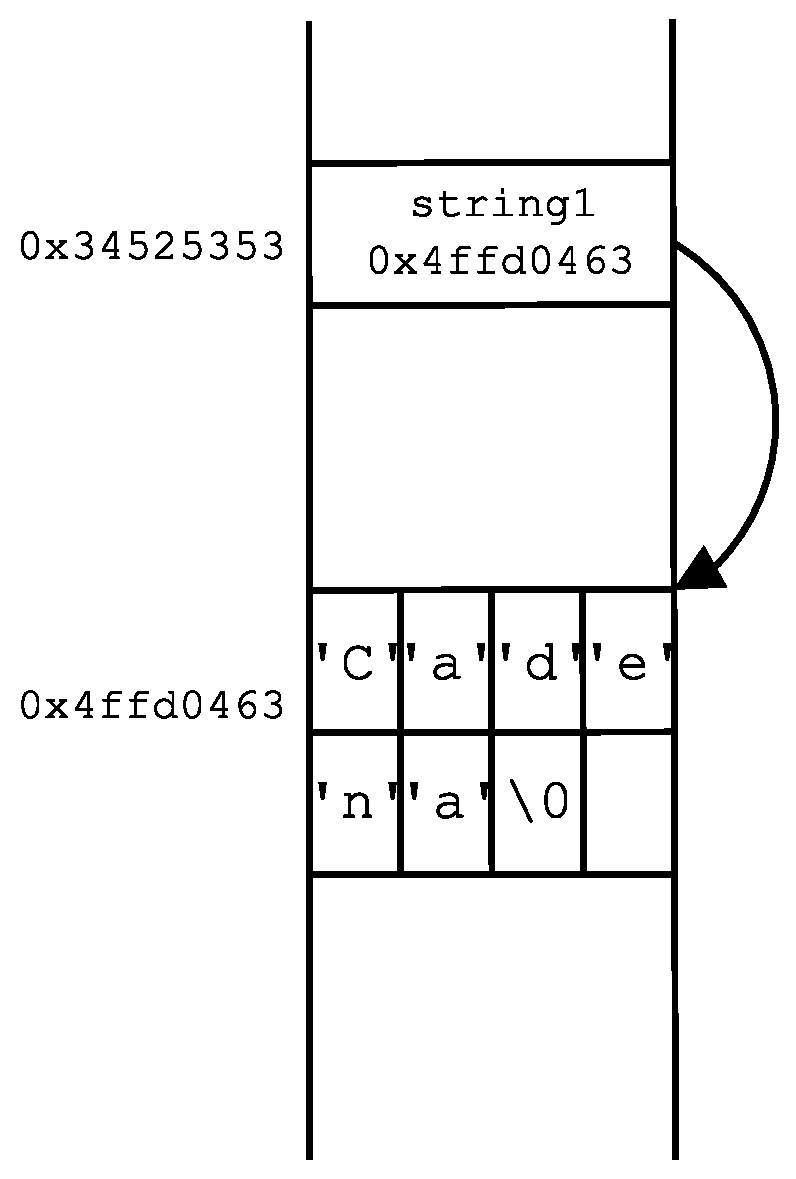
\includegraphics[height=7.5cm]{punteros/errores/cadena.eps}
    \caption{Car�cter de finalizaci�n}
  \end{center}
\end{figure}

De esta forma, en tiempo de ejecuci�n, al operar sobre una cadena
se busca el car�cter \verb+\0+, que indique el fin
de la misma. Es por esto que si se olvida poner dicho indicador 
cuando se est� rellenando una cadena car�cter a car�cter 
(en un bucle, por ejemplo), al intentar acceder a ella,
el programa seguir� leyendo la informaci�n que exista a continuaci�n
de la cadena hasta que muy probablemente intente acceder a una zona
en la que no tenga permisos y termine con el t�pico \texttt{Segmentation
Fault}.



\newpage


%%
%% LIBRER�A ESTANDAR
%%

%
% CAP�TULO: LA LIBRER�A EST�NDAR DE C
%
\chapter{La librer�a est�ndar de C}
\label{chapter:libstd}
\section {Introducci�n}

El est�ndar de C define s�lo unas pocas palabras reservadas. S�lo con
ellas no puede hacerse un programa ``normal'' en la vida real. El
programador necesita una serie de funciones y herramientas
\textbf{est�ndar}, que deben estar disponibles en cualquier entorno de
programaci�n de C / C++. A este conjunto de funciones se le llama
\textbf{librer�a est�ndar}. Las funciones se declaran en ficheros de
cabecera o \textbf{.h}. Las cabeceras contienen �nica y
exclusivamente los prototipos de las funciones. El c�digo o cuerpo de
las funciones se incluye en \textbf{ficheros objeto} que son realmente
la librer�a.

\section {Principales ficheros de cabecera}
Los principales ficheros de cabecera de C ``suelen ser'' los siguientes:

\begin{itemize}
\item
\verb+ctype.h+: Funciones �tiles para la clasificaci�n y el mapeado de c�digos.
\item
\verb+errno.h+: Funciones que permiten comprobar el valor almacenado en \texttt{errno} por algunas funciones de librer�as.
\item
\verb+float.h+: Funciones que establecen algunas propiedades de las representaciones de tipos real.
\item
\verb+limits.h+: Funciones que establecen algunas propiedades de las representaciones de tipos enteros.
\item
\verb+math.h+: Funciones que sirven para realizar operaciones matem�ticas comunes sobre valores de tipo \texttt{double}.
\item
\verb+stdarg.h+: Son declaraciones que permiten acceder a los argumentos adicionales sin nombre en una funci�n que acepta un n�mero variable de argumentos.
\item
\verb+stdio.h+: Macros y funciones para realizar operaciones de entrada y salida sobre ficheros y flujos de datos.
\item
\verb+stdlib.h+ y a veces \verb+unistd.h+: Declaraciones de una colecci�n de funciones �tiles y la definici�n de tipos y macros para usarlas. Entre ellas suele estar la funci�n \textbf{malloc} que permite hacer peticiones de memoria din�mica al sistema. 
\item
\verb+string.h+: Declaraci�n de una colecci�n de funciones �tiles para manejar cadenas y otros arrays de caracteres.
\item
\verb+time.h+: Declaraci�n de funciones para el manejo de fechas. 
\end{itemize}

\section{stdio.h}

\subsection {Funciones para el manejo de la Entrada/Salida}

\subsubsection{printf}

\verb+int printf (const char *formato, ...);+
\begin{flushleft}
Escribe texto formateado por el flujo \texttt{stdout}, seg�n las especificaciones de ``formato'' y la lista de expresiones. Devuelve el n�mero de caracteres escritos o un valor negativo en caso de error.
\end{flushleft}

\subsubsection{scanf}

\verb+int scanf (const char  *formato, ...);+
\begin{flushleft}
Lee texto por el flujo \texttt{stdin} y lo almacena seg�n las especificaciones de ``formato''. Devuelve el n�mero de valores asignados o \texttt{EOF} si se produce error o se alcanza fin de fichero sin producirse lectura.
\end{flushleft}
%
%\subsubsection{gets}
%
%\verb+char *gets(char *s);+
%\begin{flushleft}
%Lee caracteres por el flujo est�ndar de entrada ``stdin'' y los almacena en el ``array'' que comienza en ``s'' hasta que se almacena un car�cter ``NL'' o se active el indicador de error o el fin de fichero. Si almacena alg�n elemento, termina almacenando un car�cter nulo. Devuelve ``s'' si almacena alg�n car�cter. Sustituye el car�cter ``NL'' por '$\backslash$0'.
%\end{flushleft}
%
\subsubsection{puts}

\verb+int puts (const char *s);+
\begin{flushleft}
Escribe los caracteres de la cadena ``s'' por el flujo \texttt{stdout}. Escribe un car�cter ``NL'' en lugar del nulo de terminaci�n. Devuelve un valor no negativo. En caso de error devuelve \texttt{EOF}.
\end{flushleft} 

\subsection {Funciones para el manejo de ficheros}

\subsubsection{fopen}
\label{subsection:fopen}

\verb+FILE *fopen(const char *nombre_fichero, const char *modo);+ 
\begin{flushleft}
Abre el fichero de nombre ``nombre\_fichero'', lo asocia con un flujo de datos y devuelve un puntero al mismo. Si falla la llamada, devuelve un puntero nulo.
Algunos de los caracteres iniciales de ``modo'' son:
\begin {description}
\item[] ``r'', para abrir un fichero de texto existente para su lectura
\item[] ``w'', para crear un fichero de texto o abrir y truncar uno existente, para su escritura
\item[] ``a'', para crear un fichero de texto o abrir uno existente, para su escritura. El indicador de posici�n se coloca al final del fichero antes de cada escritura
\item[] ``r+'', para abrir un fichero de texto existente para su lectura y escritura
\end {description} 
\end{flushleft}

\ejemplo{libstd/ejemplo_abre_fichero.c}

\subsubsection{fclose}

\verb+int fclose(FILE *flujo);+
\begin{flushleft}
Cierra el fichero asociado con ``flujo''. Devuelve 0 en caso de �xito y \texttt{EOF} (end of file) en caso contrario.
\end{flushleft}

\ejemplo{libstd/ejemplo_cierra_fichero.c}


\subsubsection{fwrite}

\verb+size_t fwrite(const void *buffer, size_t n, size_t c, FILE *flujo);+
\begin{flushleft}
La rutina \verb+fwrite+ permite escribir c elementos de longitud n bytes almacenados en el buffer apuntado por ``flujo''.
\end{flushleft}


\ejemplo{libstd/ejemplo_fwrite.c}

\subsubsection{fread}

\verb+size_t fread(const void *buffer, size_t n, size_t c, FILE *flujo);+

\begin{flushleft}
La rutina \verb+fread+ permite leer c elementos de longitud n bytes del fichero apuntado por ``flujo'' y los almacena en el buffer especificado.
\end{flushleft}

\ejemplo{libstd/ejemplo_fread.c}

\subsubsection{fgetc}

\verb+int fgetc(FILE *flujo);+
\begin{flushleft}
Lee el siguiente car�cter por ``flujo'', avanza el indicador de posici�n y devuelve \texttt{int}. Devuelve \texttt{EOF} si pone a 1 el indicador de fin de fichero o el de error.
\end{flushleft}

\subsubsection{fgets}

\verb+char *fgets(char *s, int n, FILE *flujo);+
\begin{flushleft}
Lee caracteres por ``flujo'' y los almacena en elementos sucesivos del ``array'' que comienza en ``s'', continuando hasta que almacene ``n-1'' caracteres, almacene un car�cter del nueva l�nea o ponga a 1 los indicadores de error o de fin de fichero. Si almacena un car�cter, concluye almacenando un car�cter nulo en el siguiente elemento del ``array''. Devuelve ``s'' si almacena alg�n car�cter y no ha puesto a 1 el indicador de error; en caso contrario devuelve un puntero nulo.
\end{flushleft}

\subsubsection{fputc}

\verb+int fputc(int c, FILE *flujo);+
\begin{flushleft}
Escribe el car�cter \texttt{c} por ``flujo'', avanza el indicador de posici�n del fichero y devuelve \texttt{int c} . En caso de error devuelve \texttt{EOF}.
\end{flushleft}

\subsubsection{fputs}

\verb+int fputs(const char *s, FILE *flujo);+
\begin{flushleft}
Escribe los caracteres de la cadena \texttt{s} por ``flujo''. No escribe el car�cter nulo de terminaci�n. En caso de �xito, devuelve un valor no negativo; en caso de error devuelve \texttt{EOF}.
\end{flushleft}

\subsubsection{fscanf}

\verb+int fscanf(FILE *flujo, const char *formato, ...);+
\begin{flushleft}
Lee texto y convierte a la representaci�n interna seg�n el formato especificado en \texttt{formato}. Devuelve el n�mero de entradas emparejadas y asignadas, o \texttt{EOF} si no se almacenan valores antes de que se active el indicador de error o de fin de fichero.
\end{flushleft}

\subsubsection{fprintf}

\verb+int fprintf(FILE *flujo, const char *formato, ...);+
\begin{flushleft}
Genera texto formateado, bajo el control de formato \texttt{formato} y escribe los caracteres generados por \texttt{flujo}. Devuelve el n�mero de caracteres generados o un valor negativo en caso de error.

\end{flushleft}

\begin{flushleft}
A modo de resumen estas son las especificaciones de formato m�s comunes:
\end{flushleft}

\begin{tabular}{|c|l|}
\hline
\textbf{Formato} & \textbf{Descripci�n}\\
\hline
 \%d & Entero con signo\\
\hline
\%u & Entero sin signo\\
\hline
\%c & Caracter\\
\hline
\%s & Puntero a cadena de caracteres\\
\hline
\end{tabular}

\ejemplo{libstd/ejemplo_fprintf.c}


\subsubsection{fseek}
\verb+int fseek( FILE *flujo, long desplazamiento, int origen);+\\

La  funci�n fseek mueve el puntero de posici�n del fichero correspondiente al flujo de datos apuntado por ``flujo''.  La nueva posici�n, medida en bytes, se obtiene a�adiendo el n�mero indicado por desplazamiento a la posici�n especificada por origen. La variable origen puede tomar tres valores:

\begin{itemize}
        \item{\verb+SEEK_SET+: El puntero de posici�n apuntar� al inicio del fichero m�s el desplazamiento}
        \item{\verb+SEEK_CUR+: El puntero de posici�n apuntar� a la posici�n actual del puntero de posici�n del fichero m�s el desplazamiento.}
        \item{\verb+SEEK_END+: El puntero de posici�n apuntar� al fin del fichero m�s el desplazamiento (deber� ser menor o igual que cero).}
        
\end{itemize}

\nota{Al abrir un fichero el puntero de posici�n apunta al principio del mismo.
      Toda lectura o escritura hecha en el fichero modifica el puntero de posici�n.}

\ejemplo{libstd/ejemplo_fseek.c}

\section{stdlib.h}

\subsection{Funciones para la conversi�n de tipos}
\subsubsection{abs}

\verb+int abs(int i);+
\begin{flushleft}
Devuelve el valor absoluto de \texttt{i}.
\end{flushleft}

\subsubsection{atof}

\verb+double atof(const char *s);+
\begin{flushleft}
Convierte los caracteres de la cadena \texttt{s} a la representaci�n interna de tipo \texttt{double} y devuelve ese valor.
\end{flushleft}

\subsubsection{atoi}

\verb+int atoi(const char *s);+
\begin{flushleft}
Convierte los caracteres de la cadena \texttt{s} a la representaci�n interna de tipo \texttt{int} y devuelve ese valor.
\end{flushleft}

\subsubsection{atol}

\verb+long atol(const char *s);+
\begin{flushleft}
Convierte los caracteres de la cadena \texttt{s} a la representaci�n interna de tipo \texttt{long} y devuelve ese valor.
\end{flushleft}

\subsubsection{strtod}

\verb+double strtod(const char *s, char **finptr);+
\begin{flushleft}
Convierte los caracteres iniciales de la cadena \texttt{s} en la correspondiente representaci�n interna de tipo \texttt{double} y devuelve ese valor.
Si \texttt{finptr} no es un puntero nulo, la funci�n almacena en �l un puntero al resto de la cadena que no se ha convertido.
\end{flushleft}

\subsubsection{strtol}

\verb+long strtol(const char *s, char **finptr);+
\begin{flushleft}
Convierte los caracteres iniciales de la cadena \texttt{s} en la correspondiente representaci�n interna de tipo \texttt{long} y devuelve ese valor.
Si \texttt{finptr} no es un puntero nulo, la funci�n almacena en �l un puntero al resto de la cadena que no se ha convertido.
\end{flushleft}

\subsection{Funciones para el manejo de memoria}
\subsubsection{malloc}

\verb+void *malloc(size_t longitud);+
\begin{flushleft}
Asigna una direcci�n de memoria para un objeto de datos de tama�o \texttt{longitud} y devuelve esa direcci�n.
\end{flushleft}

\subsubsection{calloc}

\verb+void *calloc(size_t nelem, size_t longitud);+
\begin{flushleft}
Asigna una localizaci�n en memoria a un objeto de datos \textit{array} que contiene \textit{nelem} elementos de tama�o \texttt{longitud}, asignando ceros a todos los bytes del \textit{array} y devuelve la direcci�n del primer elemento en caso de �xito; en caso contrario, devuelve un puntero nulo.
\end{flushleft}

\subsubsection{realloc}

\verb+void *realloc(void *p, size_t longitud);+
\begin{flushleft}
Cambia el tama�o de la memoria apuntada por \texttt{p} al que se indica con \texttt{longitud}. Asigna una direcci�n de memoria para un objeto de datos de tama�o \texttt{longitud}, copiando los valores almacenados en \texttt{p}. Devuelve la nueva direcci�n de memoria asignada.
\end{flushleft}

\subsubsection{free}

\verb+void free(void *p);+
\begin{flushleft}
Si \texttt{p} no es un puntero nulo, la funci�n libera la memoria asignada al objeto de datos cuya direcci�n es \texttt{p}, en caso contrario, no hace nada. Se puede liberar la memoria asignada con \texttt{calloc}, \texttt{malloc}, \texttt{realloc}.
\end{flushleft}

\section{string.h}

\subsubsection{strcmp}
\label{strcmp}
\verb+int strcmp(const char *s1, const char *s2);+
\begin{flushleft}
Compara los elementos de dos cadenas \texttt{s1} y \texttt{s2} hasta que encuentra elementos diferentes. Si todos son iguales, devuelve 0. Si el elemento diferente de \texttt{s1} es mayor que el de \texttt{s2}, devuelve un valor mayor que cero; en caso contrario, devuelve un valor menor que cero.
\end{flushleft}

\subsubsection{strcpy}

\verb+char *strcpy(char *s1, const char *s2);+
\begin{flushleft}
Copia la cadena \texttt{s2}, incluyendo el nulo, en el \textit{array} de elementos \texttt{char} que comienza en \texttt{s1}. Devuelve \texttt{s1}.
\end{flushleft}

\subsubsection{strdup}

\verb+char *strdup(const char *s);+
\begin{flushleft}
Devuelve un puntero a una nueva cadena de caracteres que es un duplicado de la cadena \texttt{s}. La memoria para esta cadena de caracteres se obtiene con la funci�n malloc y se libera con la funci�n free.
\end{flushleft}

\subsubsection{strlen}

\verb+size_t strlen (const char *s);+
\begin{flushleft}
Devuelve el n�mero de caracteres de la cadena \texttt{s}, sin incluir el nulo de terminaci�n.
\end{flushleft}

\subsubsection{strncmp}

\verb+int strncmp(const char *s1, const char *s2, size\_t n);+
\begin{flushleft}
Compara los elementos de las cadenas \texttt{s1} y \texttt{s2} hasta que encuentra alguno diferente o hasta que se han comparado \texttt{n} elementos. Si todos los elementos son inguales, devuelve 0. Si el elemento diferente de \texttt{s1} es mayor que el de \texttt{s2}, devuelve un n�mero positivo. En caso contrario, devuelve un n�mero negativo.
\end{flushleft}

\subsubsection{strncpy}

\verb+char *strncpy(char *s1, const char *s2, size\_t n);+
\begin{flushleft}
Copia la cadena \texttt{s2}, sin incluir el nulo, en la cadena \texttt{s1}. Copia no m�s de \texttt{n} caracteres de \texttt{s2}. Entonces almacena, cero o m�s caracteres nulos si son necesarios para completar un total de \texttt{n} caracteres. Devuelve \texttt{s1}.
\end{flushleft}

\subsubsection{strndup}

\verb+char *strndup(const char *s, size\_t n);+
\begin{flushleft}
Devuelve un puntero a una nueva cadena de caracteres que es un duplicado de la cadena \texttt{s}, solo copia los primeros \texttt{n} caracteres, incluyendo el nulo. La memoria para esta cadena de caracteres se obtiene con la funci�n malloc y se libera con la funci�n free.
\end{flushleft}

\section{math.h}

\subsubsection{ceil}

\verb+double ceil(double x);+
\begin{flushleft}
Valor entero m�s peque�o no menor que \texttt{x}.
\end{flushleft}

\subsubsection{cos}

\verb+double cos(double x);+
\begin{flushleft}
Coseno de \texttt{x} en radianes.
\end{flushleft}

\subsubsection{exp}

\verb+double exp(double x);+
\begin{flushleft}
Exponencial de \texttt{x}, \(e^x\).
\end{flushleft}

\subsubsection{fabs}

\verb+double fabs(double x);+
\begin{flushleft}
Valor absoluto de \texttt{x}, \(\vert x \vert\).
\end{flushleft}

\subsubsection{floor}

\verb+double floor(double x);+
\begin{flushleft}
Mayor valor entero menor que \texttt{x}.
\end{flushleft}

\subsubsection{log}

\verb+double log(double x);+
\begin{flushleft}
Devuelve el logaritmo natural de \texttt{x}.
\end{flushleft}

\subsubsection{log10}

\verb+double log10(double x);+
\begin{flushleft}
Devuelve el logaritmo en base 10 de \texttt{x}.
\end{flushleft}

\subsubsection{pow}

\verb+double pow(double x, double y);+
\begin{flushleft}
Devuelve \texttt{x} elevado a la potencia \texttt{y}, \(x^y\).
\end{flushleft}

\subsubsection{sin}  

\verb+double sin(double x);+
\begin{flushleft}
Devuelve el seno de \texttt{x} (en radianes).
\end{flushleft}

\subsubsection{sqrt}

\verb+double sqrt(double x);+
\begin{flushleft}
Devuelve la ra�z cuadrada de \texttt{x}.
\end{flushleft}

\subsubsection{tan}

\verb+double tan(double x);+
\begin{flushleft}
Devuelve la tangente de \texttt{x} (en radianes). 
\end{flushleft}

\section{ctype.h}

\subsubsection{islower}

\verb+int islower (int c);+
\begin{flushleft}
Devuelve un valor distinto de cero si \texttt{c} es cualquiera de las letras min�sculas \verb+[a-z]+ u otra min�scula local.
\end{flushleft}

\subsubsection{isupper} 

\verb+int isupper (int c);+
\begin{flushleft}
Devuelve un valor distinto de cero si \texttt{c} es cualquiera de las letras may�sculas \verb+[A-Z]+ u otra may�scula local.
\end{flushleft}

\subsubsection{tolower}

\verb+tolower (int c);+
\begin{flushleft}
Devuelve la correspondiente letra min�scula si existe y si \texttt{isupper(c)} es distinto de cero; en caso contrario, devuelve \texttt{c}.
\end{flushleft}

\subsubsection{toupper}

\verb+toupper (int c);+
\begin{flushleft}
Devuelve la correspondiente letra may�scula si existe y si \texttt{islower(c)} es distinto de cero; en caso contrario, devuelve \texttt{c}.
\end{flushleft}

\newpage

%%
%% TEMAS AVANZADOS
%%

\newpage
\ \
\newpage


%
% CAP�TULO: TEMAS AVANZADOS
%
\chapter{Temas avanzados}

% Subseccion Entrada/Salida con archivos
\section{Entrada/Salida con archivos: Un peque�o tutorial}

En el cap�tulo \ref{chapter:libstd} hemos visto, de forma general, algunas de
las funciones m�s importantes proporcionadas por la librer�a est�ndar de C. Entre otras
funciones se describieron las rutinas para realizar entrada/salida con archivos. En
esta secci�n vamos a ver c�mo utilizar ese conjunto de funciones para leer
y escribir en archivos. Dado que ya hemos explicado el funcionamiento 
de cada una de las funciones necesarias nos centraremos en describir el procedimiento.



\begin{flushleft}
Los pasos fundamentales a la hora de operar con ficheros son los siguientes:
\end{flushleft}
\begin{enumerate}
        \item{Declarar una variable tipo \textit{flujo}, que representar� el fichero.}
        \item{Abrir el fichero y asociar la variable con ese fichero.}
        \item{Leer/Escribir en el fichero.}
        \item{Cerrar el fichero.}
\end{enumerate}

\begin{flushleft}
Pasaremos a describir cada uno de los pasos m�s detalladamente
\end{flushleft}

\subsection{Variables de \textit{flujo}}

La librer�a est�ndar de C tiene definido un tipo de datos, \verb+FILE *+ que representa un
\textit{flujo} de bytes. Asociado a este flujo puede estar un archivo, una posici�n de
memoria, el teclado, etc... La declaraci�n:
\begin{verbatim}
FILE *fich;
\end{verbatim}

Declara que la variable \verb+fich+ representar� un flujo de datos, que luego asociaremos.


\subsection{Abrir el fichero}
Una vez que tenemos declarada una variable de tipo \verb+FILE *+ tenemos que asociarla con el fichero
que queremos abrir. Esto se hace mediante la llamada \verb+fopen+.\\

Como se comenta en \ref{subsection:fopen}, \verb+fopen+ admite varios \textit{modos} de apertura
de ficheros. Si quisi�ramos abrir el fichero para lectura (esto es, leer los datos que contiene y no
modificarlo), utilizar�amos \verb+fopen+ de la siguiente manera:
\begin{verbatim}
fich = fopen( "fichero.txt", "r" );
\end{verbatim}

\begin{flushleft}
Si en cambio quisi�ramos crear un nuevo fichero har�amos lo siguiente:
\end{flushleft}
\begin{verbatim}
fich = fopen( "fichero.txt", "w" );
\end{verbatim}

\begin{flushleft}
Por �ltimo es posible que necesitemos a�adir datos al final de un fichero ya existente:
\end{flushleft}

\begin{verbatim}
fich = fopen( "fichero.txt", "a" );
\end{verbatim}



\subsection{Leer y escribir en un fichero}

Ya vimos en el cap�tulo \ref{chapter:libstd} algunas primitivas de entrada/salida que ofrece
la librer�a est�ndar. Veamos como se usan en la pr�ctica. 


\subsubsection{Lectura}
Leer un archivo que tenga un formato determinado es una tarea f�cil utilizando la rutina
\verb+fscanf+, que funciona de forma an�loga a \verb+scanf+. 

Supongamos que queremos leer una l�nea del fichero \verb+notas.txt+ que contiene un listado
de notas de alumnos con el siguiente formato:
\begin{verbatim}
Nombre Apellido1 Apellido2 notaParcial1 NotaParcial2
\end{verbatim}

\begin{flushleft}
El fragmento de c�digo que realizar�a esta lectura ser�a el siguiente:
\end{flushleft}

\begin{verbatim}
FILE *fich;
char nombre[10], apellido1[10], apellido2[10];
float nota1,nota2;

fich = fopen( "notas.txt", "r" );
fscanf( fich, "%s %s %s %f %f\n", nombre, apellido1, apellido2, &nota1, &nota2 );
\end{verbatim}

\nota{Tienes que tener en cuenta que la variable \texttt{fich} funciona como
un \textit{apuntador} al archivo. Cuando se realiza una lectura este apuntador
se desplaza de forma que los datos le�dos quedan \emph{por detr�s de �l}. En la 
pr�ctica esto quiere decir que para volver a leer unos datos que ya has le�do
previamente tienes que recolocar este puntero, utilizando la rutina \texttt{fseek()}}

Una necesidad com�n a la hora de leer de un archivo consiste en saber cuando 
hemos llegado al final del archivo. Esto se realiza con la rutina \verb+feof()+, que
devuelve un valor distinto de cero cuando hemos llegado al final del archivo.
El siguiente ejemplo lee todas las l�neas del archivo \verb+notas.txt+, imprimiendo
por pantalla los datos:

\ejemplo{avanzados/ejemplo_ficheros1.c}


Otra opci�n a la hora de leer de un archivo es leer un n�mero determinado de caracteres y almacenarlos
en un \textit{buffer} para posterior proceso. Esto se puede realizar con la rutina \verb+fgets+. 


\subsubsection{Escritura}

\begin{flushleft}
Para escribir sobre un archivo tenemos disponibles las siguientes primitivas:
\end{flushleft}
\begin{itemize}
        \item{\verb+fprintf+: Escritura con formato. Funcionamiento similar a \verb+printf+}
        \item{\verb+fputs+: Escribe un \textit{buffer} de caracteres en archivo especificado}
\end{itemize}

\nota{Obviamente para poder escribir sobre un archivo tenemos que abrir el mismo en modo
escritura}



\subsection{Cerrar el fichero}
Una vez que hemos terminado de operar con el fichero hay que realizar una operaci�n de
\textbf{cierre} sobre la variable asociada, utilizando la rutina \verb+fclose()+.
Una vez que hemos cerrado un fichero no podremos realizar ninguna operaci�n de lectura/escritura
sin antes volver a abrirlo.




\subsection{Ejemplo}
El siguiente ejemplo utiliza todas las operaciones vistas hasta ahora para analizar los
datos del fichero \verb+notas.txt+ (que contiene notas de alumnos, en el formato especificado
anteriormente), escribiendo los resultados en el archivo\\ \verb+notas_finales.txt+

\ejemplo{avanzados/ejemplo_ficheros2.c}



%Los ficheros, en contraposici�n con las estructuras de datos vistas
%hasta ahora (variables simples, vectores, registros, etc.), son
%estructuras de datos almacenadas en memoria secundaria. Para utilizar
%la informaci�n en memoria principal se emplea fundamentalmente la
%instrucci�n de asignaci�n; sin embargo, para guardar o recuperar
%informaci�n de un fichero es necesario realizar una serie de
%operaciones.
%El formato de declaraci�n de un fichero es el siguiente:
%
%\begin{verbatim}
%FILE * nom_var_fich;
%\end{verbatim}
%
%En otros lenguajes la declaraci�n del fichero determina el tipo de
%datos que se van a almacenar en �l. En C la filosof�a es distinta,
%todos los ficheros almacenan bytes y es cuando se realiza la apertura
%y la escritura cuando se decide c�mo y qu� se almacena en el mismo;
%durante la declaraci�n del fichero no se hace ninguna distinci�n sobre
%el tipo del mismo.\\
%
%Hasta ahora, para obtener y almacenar datos de una estructura de datos
%bastaba con realizar asignaciones a la misma. Para utilizar los
%ficheros el procedimiento es distinto. Antes de usar un fichero es
%necesario realizar una operaci�n de apertura del mismo;
%posteriormente, si se desea almacenar datos en �l hay que realizar una
%operaci�n de escritura y si se quiere obtener datos de �l es necesario
%hacer una operaci�n de lectura. Cuando ya no se quiera utilizar el
%fichero se realiza una operaci�n de cierre del mismo para liberar
%parte de la memoria principal que pueda estar ocupando (aunque el
%fichero en s� est� almacenado en memoria secundaria, mientras est�
%abierto ocupa tambi�n memoria principal).


%
% SECCI�N: L�NEA DE COMANDOS
%
\section{L�nea de comandos}

% Subseccion Introducci�n
\subsection{Introducci�n}

Seguramente habr�s tenido que ejecutar alguna vez un programa de consola que requiera
\emph{argumentos en la l�nea de comandos}, como por ejemplo \verb+ls -l /+ (linux) o 
\verb+dir /p+ (DOS/Windows). \\

Los argumentos de la l�nea de comandos no son m�s que informaci�n adicional que se le pasa al
programa a la hora de ejecutarse. En los ejemplos anteriores esta informaci�n adicional
ser�an las cadenas \verb+-l+ y \verb+/p+. En esta secci�n vamos a ver c�mo acceder a esta 
informaci�n desde nuestros programas en C.


% Subseccion El prototipo de la funci�n main
\subsection{El prototipo de la funci�n \texttt{main}}

Hasta ahora el prototipo de la funci�n \verb+main+ que hemos utilizado es el siguiente:
\begin{verbatim}
int main( void );
\end{verbatim}

Es decir, nuestra rutina \verb+main+ no admit�a ning�n par�metro, lo cual parece l�gico, ya 
que no somos nosotros quienes llamamos a esta rutina (lo hace el sistema operativo cuando
ejecutamos el programa). Sin embargo existe otro posible prototipo para esta funci�n:

\begin{verbatim}
int main( int argc, char **argv );
\end{verbatim}

Como habr�s observado hemos cambiado los argumentos que recibe la funci�n (y por tanto el programa). Estos
dos nuevos par�metros no son m�s que informaci�n acerca de la l�nea de comandos con la que se ha ejecutado
el programa. M�s concretamente:

\begin{itemize}
        
        \item{\verb+int argc+: Este par�metro contiene el n�mero de argumentos con los que el programa
        ha sido llamado. El propio programa se considera tambi�n un argumento el primero, como veremos
        m�s adelante.}

        \item{\verb+char **argv+: Array de punteros a punteros de cadenas de caracteres. Esto quiere
        decir que \verb+argv[0]+ ser� un puntero a una cadena de caracteres que conformar� el primer
        argumento del programa.}
\end{itemize}


\begin{flushleft}
Antes de seguir profundizando en el tema veamos algunos ejemplos:
\end{flushleft}



\begin{verbatim}
ls -l --color /
\end{verbatim}


\vspace{0.3cm}
\begin{tabular}{|c|c|}
\hline
\textbf{�ndice de \texttt{argv}} & \textbf{Contenido de \texttt{argv}} \\
\hline
0 & \verb+ls+ \\
\hline
1 & \verb+-l+ \\
\hline
2 & \verb+--color+\\
\hline
3 & \verb+/+\\
\hline
\end{tabular}
\vspace{0.4cm}


Cuando habl�bamos del par�metro \verb+argc+ dec�amos que conten�a el n�mero de argumentos
que se pasan a \verb+main+. Hemos de tener en cuenta que todo programa C recibe al menos un
argumento, y este es el nombre del ejecutable que contiene al programa, como se puede comprobar
f�cilmente mediante el siguiente programa:

\ejemplo{avanzados/ejemplo_argv0.c}

\begin{flushleft}
Si ejecutamos el programa sin argumentos obtenemos la siguiente salida:
\end{flushleft}

\begin{verbatim}
argc vale: 1
argv[0] es: ejemplo_argv0.exe
\end{verbatim}


Por lo tanto al manejar los argumentos de la l�nea tienes que tener en cuenta que 
\verb+argc+ siempre ser� \textbf{mayor o igual que uno}, y \verb+argv[0]+ contendr� siempre
la ruta al fichero ejecutable que contiene tu programa.\\

Veamos por �ltimo un ejemplo de un programa que act�a de forma diferente seg�n los argumentos
de l�nea de comandos que le pasemos:

\ejemplo{avanzados/ejemplo_cmdline.c}
\begin{flushleft}
�Ser�as capaz de saber como se comporta este programa sin ejecutarlo previamente?
\end{flushleft}


% Seccion Punteros a funciones
\section{Punteros a funciones}
 
\subsection{El concepto}

Esta es quiz� una de las funcionalidades que menos conoce el
programador que viene de otros lenguajes, pero que puede resultar muy
�til para resolver problemas de ``orden superior'' con una simpleza y
elegancia no muy corrientes en el paradigma imperativo.\\

Un puntero a funci�n es una variable que guarda la posici�n de memoria
de una funci�n. Por ejemplo:\\
 
\verb+void (*funcion)(void)+\\

Es un puntero a una funci�n sin argumentos, ni valor de retorno.

\subsection{�Para qu� sirven?}

Como ya vimos anteriormente, un puntero ``corriente'' nos permit�a
entre otras cosas: utilizar estructuras de datos din�micas, pasar
variables por referencia en vez de por valor.\\

Un puntero a funci�n nos permite hacer cosas m�s
``divertidas''. Podemos cargar librer�as de forma din�mica, hacer que
nuestro c�digo se automodifique en tiempo de ejecuci�n, programar
rutinas de orden superior, e implementar otra serie de funcionalidades
que amenizan nuestra tarea como desarrolladores.

\subsection{Ejemplo de orden superior}

\nota{Cuando hablamos de orden superior nos referimos a la capacidad
que tiene un lenguaje para operar con funciones como si variables
comunes se tratara. Con orden superior se puede, por ejemplo, pasar
una funci�n como argumento a otra funci�n.}

El siguiente ejemplo hace uso de la funci�n \verb+qsort()+. Dicha
funci�n reordena listas de elementos de cualquier tipo. La lista debe
ser un vector de elementos de un tama�o fijo. Por ejemplo podemos
reordenar una lista de estructuras de datos, o una simple lista de
enteros. El algoritmo quicksort es siempre el mismo. Lo �nico que
diferencia un caso de otro es el ``criterio'' de ordenaci�n de la
lista. En un caso hay que comparar dos enteros, y en el otro hay que
utilizar un criterio de comparaci�n adaptado a la estructura de
datos. Si la estructura representa la lista de empleados de una
empresa, habr� que preguntarse si queremos ordenar por nombre de
empleado, por salario o por cualquier otro criterio variopinto.\\

``El criterio'' de ordenaci�n es una funci�n que debe utilizar \verb+qsort()+
para saber c�mo ordenar las listas. Por ese motivo, \verb+qsort()+ debe
recibir un puntero a la funci�n que compare los elementos de la lista.

\ejemplo{avanzados/ejemplo_punteros_funciones.c} 

\subsection{Ejemplo de c�digo mutante}

El siguiente programa muestra un programa que se reescribe en tiempo
de ejecuci�n. Para ello primero pide 100 Bytes de memoria, despu�s
escribe en esa memoria las instrucciones correspondientes a una
funci�n, y finalmente ejecuta la funci�n con distintas variantes.

\ejemplo{avanzados/ejemplo_punteros_funciones_2.c}

El anterior ejemplo rellena unas posiciones de memoria con c�digo
m�quina. En concreto, el c�digo m�quina es equivalente a:

\begin{verbatim}   
int imprime()
{
  return 0x10;
}
\end{verbatim}   

Que en ensamblador de Intel x86 corresponde a:

\begin{verbatim}   
imprime:        
        pushl   %ebp
        movl    %esp, %ebp
        movl    $$10, %eax
        popl    %ebp
        ret          
\end{verbatim}   

y en binario Intel x86

\begin{verbatim}   
memoria[0] = 0x55;
memoria[1] = 0x89;
memoria[2] = 0xE5; 
memoria[3] = 0xB8; // mov eax <= 0x10 valor de retorno 
memoria[4] = 0x10; // 0x10
memoria[5] = 0x00; 
memoria[6] = 0x00; 
memoria[7] = 0x00;
memoria[8] = 0x5D; // ret
memoria[9] = 0xC3;
\end{verbatim}   

Para obtener el c�digo equivalente a un programa de C en ensamblador
se ha empleado: 

\begin{verbatim}   
  gcc -S fichero.c -o fichero.s # generar ensamblador
\end{verbatim}   
     
Para obtener el c�digo m�quina se ha utilizado el ensamblador:
\begin{verbatim}   
  as fichero.s -o fichero.o # generar binario
\end{verbatim}   

Y las herramientas de visualizaci�n hexadecimal
\begin{verbatim}
  hexedit fichero.o 
  hexdump -C fichero.o
\end{verbatim}   






\section{Gesti�n de bibliotecas de funciones}

\subsection{�Qu� es una biblioteca?}

\definicion{Biblioteca}{Consiste en un archivo binario que almacena el c�digo
compilado de funciones. }

El programa b�sico en Unix/Linux para gestionar bibliotecas es \textit{ar} (tambi�n
\textit{ranlib}) y sus funciones b�sicas son crear, modificar y
extraer funciones. Las bibliotecas m�s importantes que se utilizan en
el desarrollo de aplicaciones C son \textit{libc.a, libm.a, etc...}

\subsection{�Para qu� necesito una biblioteca?}

Las bibliotecas permiten almacenar en un mismo archivo el c�digo de muchas funciones. Las ventajas
de esta alternativa saltan a la vista:
\begin{itemize}
	\item{Cuando queramos utilizar una funci�n de la biblioteca no tendremos que buscar el c�digo
	y compilarlo, sino simplemente decirle al compilador d�nde puede encontrar la biblioteca}

	\item{Ayudan a la reutilizaci�n de c�digo, permitiendo que varios programas compartan
	porciones de c�digo.}

	\item{Promueven una programaci�n m�s modular.}
\end{itemize}



\subsection{Bibliotecas en Unix/Linux: \textit{ar}}
La sintaxis de \textit{ar} es la siguiente:

\begin{verbatim}
ar [-] [miembro] biblioteca [ficheros]
\end{verbatim}

Comentaremos las opciones mas importantes del ar:

\begin{itemize}
\item\texttt{d}: Borrar miembros de la biblioteca.
\item\texttt{m}: Mover un miembro de la biblioteca.
\item\texttt{p}: Imprimir un miembro de la biblioteca en el fichero est�ndar de salida.
\item\texttt{q}: A�adido r�pido.
\item\texttt{r}: Reemplazar ficheros en la biblioteca.
\item\texttt{t}: Mostrar una tabla con el contenido de la biblioteca.
\item\texttt{x}: Extraer miembros de la biblioteca.
\end{itemize}

\subsection{Ejemplo}

Imaginemos que tenemos una aplicaci�n para gestionar matrices, y
que tenemos una biblioteca en donde est�n incluidos ya varios ficheros
objeto llamada \textit{matriz.a}. Si ahora queremos darle mayor
funcionalidad a nuestra biblioteca de matrices y queremos a�adir
una funcion que por ejemplo haga la inversa de una matriz,
implementamos el fichero \textit{inver.c}, lo compilamos con:

\begin{verbatim}
$ gcc -c inver.c
\end{verbatim}

Esto nos crea el c�digo objeto, y ahora para a�adir esto a la biblioteca hacemos:

\begin{verbatim}
$ ar r matriz.a inver.o
\end{verbatim}

Situ�ndonos en el path donde se encuentra la biblioteca. Si el fichero
\textit{inver.o} se encuentra en otro directorio basta con hacer:

\begin{verbatim}
$ ar r matriz.a /home/micuenta/inver.o (por ejemplo)
\end{verbatim}

Para visualizar el contenido de una biblioteca:

\begin{verbatim}
$ ar t matriz.a
inver.o
multi.o
sum.o
\end{verbatim}

Si queremos m�s informaci�n:

\begin{verbatim}
$ ar tv matriz.a
rw-r--r-- 402/ 6  875 Oct 26 14:43 2003 inver.o
etc...
\end{verbatim}

Para extraer un modulo de la biblioteca:

\begin{verbatim}
$ ar xv matriz.a inver.o
\end{verbatim}


% seccion Llamadas al sistema: POSIX
\section{Llamadas al sistema: POSIX}

\subsection {�Qu� es POSIX?}
\label{posix}

POSIX\footnote{Portable Operating System Interface} define un est�ndar
de llamadas al sistema operativo. La librer�a est�ndar de C define
unas funciones que deben estar en cualquier entorno de desarrollo de
C. POSIX Define un est�ndar IEEE de funciones que requieren ``ayuda''
del sistema operativo. En la siguiente secci�n mostramos algunas de
ellas.

\subsection{Llamadas POSIX para gesti�n de procesos}

\subsubsection{getpid}

\verb+pid_t getpid(void);+

\begin{flushleft}
Funci�n que devuelve el identificador del proceso.
\end{flushleft}

\subsubsection{getuid}

\verb+uid_t getuid(void);+

\begin{flushleft}
Funci�n que devuelve el identificador de usuario real.
\end{flushleft}

\subsubsection{getgid}

\verb+gid_t getgid(void);+

\begin{flushleft}
Funci�n que devuelve el identificador de grupo real.
\end{flushleft}

\subsubsection{fork}

\verb+pid_t fork();+

\begin{flushleft}
Funci�n que crea un proceso hijo. Devuelve 0 al proceso hijo y el pid
del hijo al proceso padre. El proceso hijo creado es una copia exacta del padre,
excepto que recibe un valor diferente de la llamada fork, 0 en el hijo, el pid
del hijo en el padre. Devuelve un valor -1 en caso de no pod crearse el proceso
hijo.

\ejemplo{avanzados/fork.c}
\end{flushleft}

\subsubsection{execvp}

\verb+int execvp(const char *fichero, const char *argv[]);+\\

\begin{flushleft}
\texttt{execvp} es en realidad solo una funci�n de la familia de funciones
\texttt{exec}. Existen
las funci�nes \texttt{execl}, \texttt{execlp}, \texttt{execle}, \texttt{execv} y
\texttt{execvp}, pero la m�s sencilla y �til es
\texttt{execvp}.
El primer par�metro, \texttt{*fichero}, es un puntero que apunta a la ruta del programa
que queremos ejecutar, el segundo es un array de punteros a char que contiene
los par�metros que queremos pasar a dicho programa (como si lo hicieramos desde
la linea de comandos), siendo el primer par�metro el nombre del mismo programa,
y el �ltimo NULL, con lo que decimos que no quedan m�s par�metros.\\
\end{flushleft}

Estas funciones lo que hacen en realidad es cambiar completamente el programa que la
ejecuta, el cual solo conserva su pid y su tabla de ficheros abiertos. Por lo
tanto, si quisieramos que un programa nuestro ejecute un programa externo (un ls
por ejemplo), podr�amos crear un proceso hijo con \texttt{fork()} y hacer que el proceso hijo
ejecute un \texttt{exec}, convirtiendose as� en otro programa.

\nota{Como \texttt{exec} reemplaza el c�digo del programa que lo ejecuta,
\texttt{exec} nunca retorna, por
lo cual cualquier c�digo siguiente a la llamada \texttt{exec} no ejecutara, a no ser que
la llamada \texttt{exec} falle.}

Veamos un ejemplo:

\ejemplo{avanzados/execvp.c}
\subsubsection{wait}

\verb+pid_t wait(int *status);+

\begin{flushleft}
Funci�n que permite a un proceso padre esperar hasta que termine un
proceso hijo cualquiera. Devuelve el identificador del proceso hijo y
el estado de informaci�n del mismo.
\end{flushleft}

\subsubsection{waitpid}

\verb+pid_t waitpid(pid_t pid, int *status, int options);+

\begin{flushleft}
Funci�n que espera hasta termina el proceso pid.
\end{flushleft}

\subsubsection{exit}

\verb+void exit(int status);+

\begin{flushleft}
Funci�n que finaliza la ejecuci�n de un proceso indicando el estado de
terminaci�n del mismo.

\ejemplo{avanzados/exit.c} 
\end{flushleft}

\subsubsection{kill}

\verb+int kill(pid_t pid, int sig);+

\begin{flushleft}
Funci�n que env�a al proceso pid la se�al sig.
\end{flushleft}

\subsubsection{pause}

\verb+int pause(void);+

\begin{flushleft}
Funci�n que bloquea al proceso hasta la recepci�n de una se�al.
\end{flushleft}

\subsubsection{sleep}

\verb+int sleep(unsigned int seconds);+

\begin{flushleft}
Funci�n que hace que el proceso despierte cuando ha transcurrido el
tiempo establecido o cuando se recibe una se�al.
\end{flushleft}

Un ejemplo que usa varias llamadas POSIX:

\ejemplo{avanzados/posix.c}

\subsection{Llamadas POSIX para la gesti�n de memoria}

\subsubsection{brk}

\verb+size = brk (addr)+;

\begin{flushleft}
Funci�n que aumenta el tama�o de una regi�n de memoria. Coloca, si es
posible, el fin del heap en la direcci�n \verb+addr+. Supone que aumenta o
disminuye el heap del segmento de datos.
\end{flushleft}

\subsubsection{dlopen}

\verb+void *dlopen (const char *filename, int flag);+

\begin{flushleft}
Funci�n que monta una biblioteca cuyo nombre se especifica en la
cadena \verb+filename+. El par�metro flag puede tener los valores RTLD\_NOW o RTLD\_LAZY.
\end{flushleft}

\subsubsection{dlclose}

\verb+int dlclose (void *handle);+

\begin{flushleft}
Funci�n que elimina de memoria una biblioteca. Solamente la elimina
cuando no queda ning�n proceso usando la biblioteca.
\end{flushleft}

\subsection{Llamadas POSIX para la entrada/salida y el sistema de ficheros}

\subsubsection{open}

\verb+int open(char *name, int flags, mode_t mode);+

\begin{flushleft}
Funci�n que abre un fichero, devolviendo un descriptor de fichero o -1
si se produce un error. Las opciones de apertura son:
\begin{description}
\item[] O\_RDONLY: S�lo lectura.
\item[] O\_WRONLY: S�lo escritura.
\item[] O\_RDWR: Lectura y escritura.
\item[] O\_APPEND: EL puntero de acceso se desplaza al final del fichero abierto.
\item[] O\_CREAT: Si existe no tiene efecto. Si no existe lo crea.
\item[] O\_TRUNC: Trunca si se abre para escritura.
Los permisos del fichero vienen indicados por mode.
\end{description}
\end{flushleft}

\subsubsection{creat}

\verb+int creat(char *name, mode_t mode);+

\begin{flushleft}
Funci�n que crea un fichero, devuelve un descriptor de fichero o -1 si
se produce un error. El fichero se abre s�lo para lectura. Si no existe se crea un fichero
vac�o.
\end{flushleft}

\subsubsection{read}

\verb+ssize_t read(int fd, void *buf, size_t n_bytes);+

\begin{flushleft}
Funci�n que lee de un fichero (descriptor de fichero), devuelve el
n�mero de bytes leidos o -1 si se produce un error. Transfiere n\_bytes
como m�ximo. Puede leer menos datos de los
solicitados si se rebasa el fin de fichero o se interrumpe por una
se�al. 

\end{flushleft}

\subsubsection{write}

\verb+ssize_t write(int fd, void *buf, size_t n_bytes);+

\begin{flushleft}
Funci�n que escribe en un fichero (descriptor de fichero), devuelve el
n�mero de bytes escritos o -1 si se produce un error. Transfiere n\_bytes
como m�ximo. Puede escribir menos datos de los
solicitados si se rebasa el tama�o m�ximo de un fichero o se
interrumpe por una se�al.
\end{flushleft}

\subsubsection{close}

\verb+int close(int fd);+

\begin{flushleft}
Funci�n que cierra un descriptor de fichero, devuelve 0 o -1 si se
produce un error. El proceso pierde la asociaci�n entre el descriptor y el fichero.
\end{flushleft}

\subsubsection{dup}

\verb+int dup(int fd);+

\begin{flushleft}
Funci�n que duplica un descriptor de fichero, devuelve un descriptor
de fichero que comparte todas las propiedades del fd o -1 si se produce
un error.
\end{flushleft}

\subsubsection{opendir}

\verb+DIR *opendir(char *dirname);+

\begin{flushleft}
Funci�n que abre un directorio, devuelve un puntero para utilizarse en
\verb+readdir()+ o \verb+closedir()+. Si se produce un error devuelve
NULL.
\end{flushleft}

\subsubsection{readdir}

\verb+struct dirent *readdir(DIR *dirp);+

\begin{flushleft}
Funci�n que realiza la lectura de entradas de un directorio, devuelve
un puntero a un objeto del tipo struct dirent que representa una
entrada de directorio o NULL si se produce un error.
\end{flushleft}

\subsubsection{closedir}

\verb+int closedir(DIR *dirp);+

\begin{flushleft}
Funci�n que cierra un directorio, devuelve un cero o un -1 si se produce un error.
\end{flushleft}

\subsubsection{mkdir}

\verb+int mkdir(char *name, mode_t mode);+

\begin{flushleft}
Funci�n que crea un directorio de nombre name, devuelve un cero o un
-1 si se produce un error.
\end{flushleft}

\subsubsection{rmdir}

\verb+int rmdir(char *name);+

\begin{flushleft}
Funci�n que borra un directorio de nombre name si est� vac�o. Si no
est� vac�o no se borra. Devuelve un cero o un -1 si se produce un
error.
\end{flushleft}

\subsubsection{link}

\verb+int link(char *existing, char *new);+

\begin{flushleft}
Funci�n que crea una entrada de directorio. Crea un nuevo enlace
f�sico para un fichero existente. Devuelve cero o un -1 si se produce
un error. \verb+existing+ no debe ser el nombre de un directorio salvo que se
tenga privilegio suficiente y la implementaci�n soporte el enlace de
directorios.
\end{flushleft}

\subsubsection{symlink}

\verb+int symlink(char *oldpath, char *newpath));+

\begin{flushleft}
Funci�n que crea una entrada de directorio. Crea un nuevo enlace
simb�lico para un fichero existente. Devuelve cero o un -1 si se
produce un error.
\end{flushleft}

\subsubsection{unlink}

\verb+int unlink(char *name);+

\begin{flushleft}
Funci�n que elimina la entrada de directorio name. Devuelve cero o un
-1 si se produce un error.
\end{flushleft}

\subsubsection{chdir}

\verb+int chdir(char *name);+

\begin{flushleft}
Funci�n que modifica el directorio actual, aquel a partir del cual se
forman los nombres relativos. Devuelve cero o un -1 si se produce un
error.
\end{flushleft}

\subsubsection{rename}

\verb+int rename(char *old, char *new);+

\begin{flushleft}
Funci�n que cambia el nombre del fichero \verb+old+ por \verb+new+, devuelve cero o
un -1 si se produce un error.
\end{flushleft}

\subsubsection{umask}

\verb+mode_t umask(mode_t cmask);+

\begin{flushleft}
Funci�n que asigna la m�scara de creaci�n de ficheros del proceso que
la invoca. Devuelve un cero o un -1 si se produce un error.
\end{flushleft}

\subsubsection{chmod}

\verb+int chmod(char *name, mode_t mode);+

\begin{flushleft}
Funci�n que modifica los bits de permiso y los bits SETUID y SETGID
del fichero. Devuelve un cero o un -1 si se produce un error. S�lo
el propietario del fichero puede cambiar estos bits.
\end{flushleft}

\subsubsection{chown}

\verb+int chown(char *name, uid_t owner, gid_t group);+

\begin{flushleft}
Funci�n que modifica el identificador de usuario y del grupo de un
fichero. Devuelve un cero o un -1 si se produce un error.
\end{flushleft}

\subsubsection{utime}

\verb+int utime(char *name, struct utimbuf *times);+

\begin{flushleft}
Funci�n que cambia las fechas de �ltimo acceso y �ltima modificaci�n
seg�n los valores de la estructura \verb+struct+ \verb+utimbuf+. Devuelve cero o un
-1 si se produce un error.
\end{flushleft}


\newpage

%%
%% HOJA DE REFERENCIA
%%

\newpage
\ \
\newpage


%
% CAP�TULO: MATERIAL DE REFERENCIA
%
\appendix
\chapter{Material de referencia}

% seccion Construcciones equivalentes ADA-C
\section{Construcciones equivalentes ADA-C}

\subsection{Introducci�n}

En esta secci�n se pretende poner de manifiesto las diferencias y similitudes 
entre los lenguajes Ada y C. Estas diferencias est�n motivadas por la orientaci�n 
radicalmente diferente de estos lenguajes. Ada un lenguaje es orientado a objetos 
y fue dise�ado para sistemas empotrados y cr�ticos, donde es muy importante la correcci�n del c�digo (vidas humanas pueden depender de ello). Es por ello que es muy "verboso", es decir, 
las instrucciones son muy largas y pesadas\footnote{Una de las ideas en su desarrolo fue la de que el c�digo se escribe una vez, pero se lee muchas}. 
El lenguaje C sin embargo fue dise�ado inicialmente para programar sistemas operativos, es decir, 
programaci�n cerca de la m�quina
(aunque dada su enorme flexibilidad se use para todo tipo de tareas), 
por lo que su sintaxis es muy escueta y expresiva.

\subsection{Sintaxis Ada vs. Sintaxis C}

Al llegar a este punto, todo lo aqu� expuesto resultar� conocido, pero
no est� de mas recapitular un poco. 
%Si habeis seguido el curso de C con atenci�n, todo lo que ve�is en
%esta secci�n ya os resultar� conocido. En caso de que teng�is alguna
%duda, remitiros a los apartados de sintaxis de C que ten�is en la
%documentaci�n.\\
Para seguir un orden comenzaremos con la declaraci�n de variables,
tipos y las cabeceras ``headers'' que se incluyen en los programas. Luego
se ver�n las sentencias de selecci�n (\texttt{if}) y de
iteraci�n (\texttt{for y while}). Finalmente se abordar� uno de los
temas m�s candentes de C pero no tanto en Ada, los punteros. Finalizando con funciones y procedimientos.

\subsubsection{Tipos, Variables y Headers}

Como hemos visto, en C existen casi los mismos tipos b�sicos que en Ada. Decimos
casi, porque hay que excluir el tipo boolean que en C no est�
predefinido\footnote{Aunque siempre se puede emular
mediante una directiva \texttt{define}}. Para ``arreglarlo'' C toma el valor 0 como True y los
dem�s como False. Por otra parte Ada incluye muchos tipos avanzados o de prop�sito espec�fico 
(n�meros complejos, duraciones, numeros en coma fija\ldots).
No olvidemos que Ada es un lenguaje enorme, con muchisimos identificadores, mientras que C es todo lo contrario.\\

\begin{flushleft}
Otra diferencia est� en la forma en que se identifican los tipos. As� pues
tenemos:\\
\end{flushleft}

\begin{tabular}{|c|c|}
\hline
\textbf{Tipo en Ada} & \textbf{Tipo en C}\\
\hline
Integer & int\\
\hline
Character & char\\
\hline
Natural & ---\\
\hline
Positive & ---\\
\hline
\end{tabular}
\vspace{0.4cm}

A la hora de declarar variables, en C se indica primero de qu�
tipo es (\verb+int+, \verb+char+, \verb+float+\ldots) y luego se escribe el nombre de la
variable. En cambio en Ada primero se indica el nombre de
la variable, seguido de un espacio, dos puntos y por �ltimo el tipo:\\

\begin{tabular}{|c|c|}
\hline
\textbf{Variable en Ada} & \textbf{Variable en C}\\
\hline
\verb+numero : Integer;+ & \verb+int numero;+\\
\hline
\verb+letra : Character;+ & \verb+char letra;+\\
\hline
\end{tabular} 
\vspace{0.4cm}

Para las tuplas, ternas,\ldots  en Ada se usa la palabra reservada
\verb-record- mientras que en C se denominan estructuras y se
definen con la palabra reservada \verb-struct-. Tomemos por ejemplo
la definici�n de un punto (en dos dimensiones) en los dos lenguajes:\\

\begin{tabular}{|l|l|}
\hline
\textbf{Punto en Ada} & \textbf{Punto en C}\\
\hline
\verb+type Tipo_Punto is record+ & \verb+struct Tipo_Punto+\\
\ \ \ \verb+x : Integer;+ & \verb+{+\\
\ \ \ \verb+y : Integer;+ & \ \ \ \verb+int x, y;+\\
\verb+end record;+ & \verb+}+\\
\hline
\end{tabular}
\vspace{0.4cm}

En cuanto a los arrays en Ada primero se indica el nombre y luego se
dice que es un array \textbf{is array}, despu�s se indica la longitud
y finalmente se indica el tipo de datos que conforman el array. En C
es m�s corto, se indica el tipo de datos, luego el nombre y por
�ltimo la longitud:\\

\begin{tabular}{|c|c|}
\hline
\textbf{Array en Ada} & \textbf{Array en C}\\
\hline
\verb+Nombre is array (desde..hasta) of Tipo_Dato;+ & \verb+tipo_dato nombre [longitud];+\\  
\hline
\verb+Whatever is array (1..25) of Integer;+ & \verb+int whatever[25];+\\ 
\hline
\end{tabular}
\vspace{0.4cm}

Hay que tener en cuenta que en C el primer elemento del array es el que ocupa la posici�n 0
 (array[0]) y para Ada en este caso es el elemento 
que ocupa la posici�n 1 (array(1)), hay que notar que a diferencia de C, 
Ada no obliga a que los arrays empiecen en 0, pueden empezar en cualquier entero, 
incluso negativo (se pueden incluso declarar con el rango de otra variable).\\

Para incluir las cabeceras:\\

\begin{tabular}{|l|l|}
\hline
\textbf{Headers en Ada} & \textbf{Headers en C}\\
\hline
\verb+with fichero; use fichero;+ & \verb+#include "fichero"+\\  
\hline
\verb+with Ada.Text_IO; use Ada.Text_IO;+ & \verb+#include <stdio.h>+\\ 
\hline
\end{tabular}

\subsubsection{Sentencias de selecci�n y de iteraci�n}

\begin{flushleft}
\textbf{Sentencia if}\\
\end{flushleft}

\begin{tabular}{|l|l|}
\hline
\textbf{if en Ada} & \textbf{if en C}\\
\hline
if condicion then & if (condicion)\\ 
\ \ ejecutar\_uno; & \{\\
else & \ \ ejecutar\_uno; \\
\ \ ejecutar\_dos; & \}\\
end if; & else \\
\ & \{\\
\ & \ \ ejecutar\_dos;\\
\ & \}\\
\hline
\end{tabular}
\vspace{0.4cm}

En C es necesario que la condici�n vaya siempre entre par�ntesis y no
se usa \verb-then- ni \verb-end if- sino llaves \textbf{\{ \}}.\\

\begin{flushleft}
\textbf{Bucle while}\\
\end{flushleft}

\begin{tabular}{|l|l|}
\hline
\textbf{while en Ada} & \textbf{while en C}\\
\hline
while condicion loop & while (condicion) \\
\ \ ejecutar\_sentencias; & \{\\
end loop; & \ \ ejecutar\_sentencias;\\ 
\ & \}\\
\hline
\end{tabular}
\vspace{0.4cm}

Al igual que en el \textbf{if}, en C los par�ntesis en la condici�n
son necesarios. \\

\begin{flushleft}
\textbf{Bucle for}
\end{flushleft}

\begin{tabular}{|l|l|}
\hline
\textbf{for en Ada} & \textbf{for en C}\\
\hline
\verb+for I in 1 .. n loop+ & \verb-for (i=0; i<n; i++)- \\
\ \ ejecutar\_sentencias; & \{\\
\verb+end loop;+ & \ \ ejecutar\_sentencias;\\ 
\ & \}\\
\hline
\end{tabular}
\vspace{0.4cm}

La principal diferencia, es que el iterador i en C tiene que estar
definido con anterioridad. Por otra parte, en C para hacer que el �ndice decremente
habr�a que poner \verb+i--+ y en Ada a�adir�amos la palabra \verb-reverse-. 

\subsubsection{Punteros}

Los punteros son muy importantes en C, y son la base de su incre�ble flexibilidad
(y tambi�n de gran parte de los quebraderos de cabeza a la hora de depurar). En Ada
se les da un uso mucho menos marcado. Por ejemplo, en C se usan para el paso 
de par�metros por refencia en la invocaci�n de funciones mientras que en Ada se usa la 
palabra reservada \verb-inout-. 
Los punteros se definen con el t�rmino \verb-access- y en C usando ``*''. 
Para acceder a la informaci�n apuntada en C hay que desreferenciar el puntero
y en Ada acceder a \texttt{nombrepuntero.all}.\\

En Ada los punteros no apuntan a un tipo b�sico tal como \verb-character- o \verb-integer-, 
sino a un \verb-record-, formado por (contenido, siguiente\_elemento). 
Aqu� radica otra de las diferencias entre ambos lenguajes:\\

\begin{tabular}{|l|l|}
\hline
\textbf{Ada} & \textbf{C}\\
\hline
\verb+nombre.all.campo+ & \verb+nombre->campo+ \\
\hline
\end{tabular}
\vspace{0.4cm}

Algo importante que tiene C y que no tiene equivalente en Ada es la aritm�tica de punteros.

\subsubsection{Funciones}

En C s�lo hay funciones, no hay procedimientos propiamente dichos, Lo
m�s parecido son las funciones que no devuelven nada (\texttt{void}). La
diferencia es que los datos no se pueden pasar como \verb-in-,  \verb-out- o \verb-inout-,
sino como variables normales (que ``mueren'' al final de la ejecuci�n
de la funci�n). Si no queremos que esto ocurra, los par�metros se han
de pasar por referencia (usando punteros)\footnote{En C++ se puede hacer de manera algo m�s comoda.}.\\

\begin{flushleft}

\begin{tabular}{|l|l|}
\hline
\textbf{Funci�n en Ada} & \textbf{Funci�n en C}\\
\hline
\verb+Function nombre (parametros) RETURN tipo_devuelto IS+ &\verb+tipo_devuelto nombre(parametros)+ \\
\ \ \ ... & \{ \\
\verb+end nombre;+ & \ \ \ ...\\
\ & \}\\
\hline
\end{tabular}
\vspace{0.8cm}
\\
De nuevo, se ve el uso de \textbf{\{ \}} frente a \verb-end-.
\end{flushleft}

\nocite{Marshall}

\newpage
\ \
\newpage
\bibliographystyle{alpha}
\bibliography{biblio/biblio}
\nocite{*}



\end{document}
